%%%%%%%%%%%%%%%%%%%%%%% file template.tex %%%%%%%%%%%%%%%%%%%%%%%%%
%
% This is a general template file for the LaTeX package SVJour3
% for Springer journals.          Springer Heidelberg 2010/09/16
%
% Copy it to a new file with a new name and use it as the basis
% for your article. Delete % signs as needed.
%
% This template includes a few options for different layouts and
% content for various journals. Please consult a previous issue of
% your journal as needed.
%
%%%%%%%%%%%%%%%%%%%%%%%%%%%%%%%%%%%%%%%%%%%%%%%%%%%%%%%%%%%%%%%%%%%
%
% First comes an example EPS file -- just ignore it and
% proceed on the \documentclass line
% your LaTeX will extract the file if required
\begin{filecontents*}{example.eps}
%!PS-Adobe-3.0 EPSF-3.0
%%BoundingBox: 19 19 221 221
%%CreationDate: Mon Sep 29 1997
%%Creator: programmed by hand (JK)
%%EndComments
gsave
newpath
  20 20 moveto
  20 220 lineto
  220 220 lineto
  220 20 lineto
closepath
2 setlinewidth
gsave
  .4 setgray fill
grestore
stroke
grestore
\end{filecontents*}
%
\RequirePackage{fix-cm}
%
%\documentclass{svjour3}                     % onecolumn (standard format)
%\documentclass[smallcondensed]{svjour3}     % onecolumn (ditto)
\documentclass[smallextended]{svjour3}       % onecolumn (second format)
%\documentclass[twocolumn]{svjour3}          % twocolumn
%
\smartqed  % flush right qed marks, e.g. at end of proof
%
\usepackage{graphicx}
\usepackage{multirow}
%
% \usepackage{mathptmx}      % use Times fonts if available on your TeX system
%
% insert here the call for the packages your document requires
%\usepackage{latexsym}
% etc.
%
% please place your own definitions here and don't use \def but
% \newcommand{}{}
%
% Insert the name of "your journal" with
% \journalname{myjournal}
%
%Example for automatically rescaling equations. 
% This is very tricky.
%\begin{equation}
%\label{eq:pimax}
%\resizebox{.55\textwidth}{!}{$
%\begin{split}
%P(\jtable_{2}|\set{E},\ttable) \propto &
%P(\keys = [jack,101],\it{Gr} = A, \it{Sat} = 1|\it{Int} = \class, \it{Rank} = 1, \it{Rat} = 3, \it{Diff}=1)\\
%\times & P(\keys = [jack,102],\it{Gr} = B, \it{Sat} = 2|\it{Int} = \class, \it{Rank} = 1, \it{Rat} = 2, \it{Diff}=2).
%\end{split}$
%}
%\end{equation}

%\usepackage{times}
%\usepackage[normaltitle,normalbib,normalmargins,normalindent]{savetrees}
\usepackage{amsmath}
\usepackage{amsfonts}
\usepackage{amssymb}
\usepackage{graphicx}
\usepackage{url}
%\usepackage{subfigure}
\usepackage{epstopdf}
\setcounter{MaxMatrixCols}{30}
%\usepackage{algorithm}
%\usepackage{algorithmic}
\usepackage{subfigure}
%\usepackage{subcaption}
\usepackage{fancyhdr}
\graphicspath{{../}{figures/}}
\usepackage{todonotes}

\DeclareMathOperator*{\argmax}{argmax}
\DeclareMathOperator*{\argmin}{argmin}
%\DeclareMathOperator{\pattern}{\pi}
\DeclareMathOperator{\Poly}{\mathbf{\mathrm{P}}}
\DeclareMathOperator{\RP}{\mathbf{\mathrm{RP}}}
%\DeclareMathOperator{\FP}{\mathbf{\mathrm{FP}}}
\DeclareMathOperator{\NP}{\mathbf{\mathrm{NP}}}
%\DeclareMathOperator{\E}{\mathbb{E}}
\renewcommand{\d}{\mathbf{d}}

\newcommand{\ZZ}{\mathbf{Z}}

\newcommand{\indep}{\ensuremath{\perp{}\!\!\!\!\!\!\!\perp{}}}
\newcommand{\dep}{\ensuremath{{\perp{}\!\!\!\!\!\!\!\not  \perp{}}}}
%\renewcommand{\L}{\mathcal{L}}
% variables denoting sets of nodes
\newcommand{\V}{V} 
\newcommand{\partC}{\mathcal{C}}
\newcommand{\pattern}{\pi}
% variables denoting nodes
\newcommand{\B}{B}
\renewcommand{\P}{P}
\newcommand{\R}{R}
\newcommand{\X}{X}
\newcommand{\Y}{Y}
\newcommand{\Z}{Z}
\newcommand{\F}{F}
\newcommand{\U}{U}
\newcommand{\W}{W}
\renewcommand{\S}{S}
\newcommand{\C}{C}
\newtheorem{mydef}{Proposition}
%variables for values
%\newcommand{\u}{u}
\renewcommand{\a}{a}
\renewcommand{\b}{b}
\newcommand{\z}{z}
\renewcommand{\v}{v}
\newcommand{\x}{x}
\newcommand{\y}{y}
\newcommand{\p}{p}
\newcommand{\s}{s}
\newcommand{\w}{w} % weights


%statistics
\newcommand{\divergence}{\it{D}}
\newcommand{\score}{\it{score}}
\newcommand{\confidence}{\it{conf}}
\newcommand{\support}{\it{support}}
\newcommand{\loglikelihood}{\it{LOG}}
\newcommand{\lof}{\it{LOF}}
\newcommand{\llmetric}{-L}
\newcommand{\lr}{\it{LR}}
\newcommand{\kl}{\it{KL}}
\newcommand{\el}{\it{EL}}
\newcommand{\mi}{\it{MI}}
\renewcommand{\mid}{\it{ELD}}
\newcommand{\jid}{\it{JID}}
\newcommand{\roc}{\it{ROC}}
\newcommand{\outrank}{\it{OutRank}}
\newcommand{\knn}{\it{KNNOutlier}}
\newcommand{\auc}{\it{AUC}}
\newcommand{\eld}{\it{ELD}}
\newcommand{\fd}{\it{FD}}
\newcommand{\parameter}{\theta}
\newcommand{\parameters}{\bs{\parameter}}
\newcommand{\bic}{\mathit{BIC}}
%random variables and graphical models
% number of values in the domain of a random variable
% variables for BNs
\newcommand{\domvals}{k}
\newcommand{\nodevalue}{\v}
\newcommand{\parvalue}{\mathbf{\pi}} % a single assignment of values to a set of 
%parents
\newcommand{\parvals}{l} % number of values of parent state.
\renewcommand{\r}{r} % CP-table row
\newcommand{\nbhd}{{\mathsf {nbdh}}}
\newcommand{\child}{\mathit{child}}
\newcommand{\parent}{\mathit{pa}}
\newcommand{\parents}{\mathbf{pa}}
\newcommand{\Parents}{\mathbf{PA}}
\newcommand{\family}{F} % families, family formulas
\newcommand{\vpi}{\mathbf{pa}} % for vectors of variable assignments
\renewcommand{\l}{\ell} % class label
\newcommand{\states}{r} % number of states of a variable
%\newcommand{\value}{value}
\newcommand{\mb}{\set{mb}} % markov blanket of a variable, vector-valued
\newcommand{\ssize}{N} % number of rows in join table; size of sample
\newcommand{\mbstates}{m} % number of states in Markov blanket
\newcommand{\frequency}{fr}
\newcommand{\pseudo}{\ast}
\newcommand{\counts}{+}
\newcommand{\weighted}{\ast}
\newcommand{\halpern}{H}
\newcommand{\Thetaa}{\theta}
\newcommand{\instance}{I}

%logic notation
%\newcommand{\predicate}{\phi}
\newcommand{\functor}{f}
\newcommand{\outdomain}{V}
\newcommand{\indomain}{\Omega}
\newcommand{\variable}{X} % first-order variable
\newcommand{\population}{\mathcal{P}}
\newcommand{\entity}{x}
\newcommand{\formula}{\phi}
\newcommand{\formulas}{\mathcal{\phi}}
\newcommand{\literal}{l}
\newcommand{\conjunction}{\set{C}} % conjunction of literals
\newcommand{\fterm}{\f} % open function term
\newcommand{\fterms}{F} % set of function terms, also nodes in JBN
\newcommand{\term}{\sigma}
\newcommand{\Terms}{\bs{\sigma}}
\newcommand{\constant}{a}
\newcommand{\constants}{\bs{\constant}}
\newcommand{\gterm}{g} % ground term
\newcommand{\gterms}{\bs{\gterm}} %list of ground terms
\newcommand{\vterm}{x} % variable term
\newcommand{\vterms}{\bs{\vterm}} % list of variable terms
\newcommand{\assign}{A} % assignment of values to Bayes net
\newcommand{\resultset}{\mathbb{R}}
\newcommand{\grounds}{\#}
\newcommand{\grounding}{\gamma}
\newcommand{\groundall}{\Gamma}
\newcommand{\vars}{\mathit{Var}} % variables in a conjunction
\newcommand{\igraph}{I} % instance-level dependency graph.
\newcommand{\assignment}{\set{a}}
\newcommand{\atom}{\ell}
\newcommand{\gnode}{\alpha}
\newcommand{\gfamily}{\ground{f}}
\newcommand{\numformulas}{m}
\newcommand{\structure}{\mathcal{S}}
% logic programs
\newcommand{\program}{\mathcal{B}}
\newcommand{\clause}{\mathcal{c}}
\newcommand{\head}{\mathit{head}}
\newcommand{\body}{\mathit{body}}
\newcommand{\crule}{\mathit{cr}} % combining rule
\newcommand{\level}{\mathit{level}} % rank of function symbols in LP

%datbase schema
\newcommand{\rcolumns}{R}
\newcommand{\ecolumns}{E}
\newcommand{\dtable}{T} % can't use \table. Generic database table
\newcommand{\datatable}{D} % generic data table, not necessarily part of database.
\newcommand{\jtable}{J} % join table
\newcommand{\Ejoin}{$J^{+}$}
\newcommand{\jtables}{m}
\newcommand{\rtable}{R} % relationship table
\newcommand{\etable}{E} % entity table.
\newcommand{\ttable}{X} % target table
\newcommand{\nextended}{n}
\newcommand{\row}{r}
\newcommand{\rows}{\mathit{rows}}
\newcommand{\col}{j}
\newcommand{\cols}{\mathit{cols}}
\newcommand{\unary}{\f} % to denote a unary or attribute function
\newcommand{\numatts}{u} % to denote the number of unary or attribute functions.
\newcommand{\g}{g} % alternative for function
\newcommand{\relational}{\mathbf{r}} % denotes a generic relational functors, can be both relationship or descriptive attribute of relationship
\newcommand{\Relation}{R} % denotes a generic boolean relation
% a special type of literal conjunction that assigns a value %to each variable
\providecommand{\keywords}{\textbf{keywords: }}
\newcommand{\loss}{\ell}
\newcommand{\class}{c} % the class attribute
\newcommand{\classlabel}{y} % the class label
\newcommand{\classifier}{\mathcal{M}}
\newcommand{\target}{t} % target object
\newcommand{\Target}{T}
\newcommand*\rfrac[2]{{}^{#1}\!/_{#2}}
\newcommand{\object}{o}
\newcommand{\Class}{C}
\newcommand{\scorediff}{\Delta}
\newcommand{\model}{B}
\newcommand{\modelprob}{\theta}
\newcommand{\profile}{P}
% the probabilities defined by a model, like conditional probabilities in a BN
\newcommand{\Targetcount}{\Gamma}
\newcommand{\neighbor}{n}
\newcommand{\feature}{V} % feature or desc attribute of object or link
\newcommand{\features}{\bs{v}} % features 
\newcommand{\Features}{\bs{V}}
\newcommand{\attribute}{a} % nonclass attribute of target object
\newcommand{\attributes}{\bs{a}}
\newcommand{\rels}{\bs{R}} % chain of relationships.
\newcommand{\maxpath}{\rho}
\newcommand{\eatts}{\it{1Nodes}}
\newcommand{\ratts}{\it{2Nodes}}
\newcommand{\atts}{\it{ANodes}}
\newcommand{\marginalize}{\it{margin}}
%special functions
\newcommand{\AVG}{\it{AVG}}
\newcommand{\instances}{n} % counts number of occurrences in DB
\newcommand{\prob}{p} % frequency of formula true in in DB

%variables denoting graphs or models
\newcommand{\mln}{M}
\newcommand{\G}{G}
\newcommand{\node}{V}
\newcommand{\nodes}{V}
\newcommand{\edges}{E}
\newcommand{\clique}{C}
\newcommand{\cliques}{\mathcal{\clique}}
\newcommand{\cliquevalue}{c}
\newcommand{\graph}{G}
\newcommand{\M}{M}
\newcommand{\J}{J}
\renewcommand{\H}{H}
\newcommand{\K}{K} % component
\renewcommand{\O}{O} % oracle
\renewcommand{\path}{\rho} % path, also foreignkey path
% Markov nets
\newcommand{\potential}{\Psi}
% database schema
\newcommand{\type}{\tau} % to denote a generic type
\newcommand{\E}{E} % for entity tables
\newcommand{\e}{e} % for specific entities
\newcommand{\f}{f}
\newcommand{\new}{\it{new}}
\renewcommand{\c}{c}
\renewcommand{\R}{R} % for relationship tables
\newcommand{\A}{A} % for attributes
\newcommand{\T}{T} % for tables generically
\newcommand{\New}{N}
\newcommand{\D}{\mathcal{D}} % for database instance
\newcommand{\databases}{\set{D}} % the number of databases
\newcommand{\vocab}{\mathcal{\L}} % for logical vocabulary associated with database
\newcommand{\name}{\mathit{name}} % generic attribute
\newcommand{\dom}{\mathit{dom}} % domain of attributes
\newcommand{\etables}{\alpha} % entity tables
\newcommand{\rtables}{\beta} % relationship table number
% specific constructs for examples


\newcommand{\team}{\it{T}}
\newcommand{\player}{\it{P}}
\newcommand{\match}{\it{M}}


\newcommand{\director}{\it{Director}}
\newcommand{\movie}{\it{Movie}}
\newcommand{\user}{\it{User}}
\newcommand{\corr}{\it{\rho}}
\newcommand{\student}{\mathit{Student}}
\newcommand{\I}{\mathit{I}}
\newcommand{\course}{\mathit{Course}}
\newcommand{\prof}{\mathit{Professor}}
\newcommand{\person}{\mathit{Person}}
\newcommand{\TA}{\mathit{TA}}
\newcommand{\actor}{\mathit{Actor}}
\newcommand{\age}{\mathit{age}}
\newcommand{\intelligence}{\mathit{intelligence}}
\newcommand{\diff}{\mathit{difficulty}}
\newcommand{\reg}{\mathit{Registered}}
\newcommand{\win}{\it{win}}
\newcommand{\ra}{\mathit{RA}}
\newcommand{\bt}{\mathit{blood type}}
\newcommand{\grade}{\mathit{grade}}
\newcommand{\gpa}{\mathit{gpa}}
\newcommand{\jack}{\mathit{Jack}}
\newcommand{\jill}{\mathit{Jill}}
\newcommand{\smith}{\mathit{Smith}}
\newcommand{\cmpt}{\mathit{CMPT120}}
\newcommand{\hi}{\mathit{Hi}}
% various constants
\newcommand{\true}{\mathit{T}}
\newcommand{\false}{\mathit{F}}
\newcommand{\normalconstant}{Z} % the normalization constant

% orderings
\newcommand{\pred}{\mathit{pred}}
%procedure names and such
\newcommand{\join}{\textsc{Join-Frequencies}}
\newcommand{\linus}{\textsc{Linus }}
\newcommand{\foil}{\textsc{Foil }}
\newcommand{\MLN}{\textsc{MLN}}
\newcommand{\treetilde}{\textsc{TILDE }}

%%%
%undirected models
\newcommand{\pot}{\phi} % potential function
%\newcommand{\theHalgorithm}{\arabic{algorithm}}
\newcommand{\test}{test}
\def\set#1{\mathbf{#1}}
\def\bs#1{\boldsymbol{#1}}
\def\ground#1{\overline{#1}}


\begin{document}

\title{Model-based Outlier Detection for Object-Relational Data%\thanks{Grants or other notes
%about the article that should go on the front page should be
%placed here. General acknowledgments should be placed at the end of the article.}
}
\subtitle{Ranking Individuals by Group Comparisons}

%\titlerunning{Short form of title}        % if too long for running head

\author{Fatemeh Riahi        \and
        Oliver Schulte %etc.
}

%\authorrunning{Short form of author list} % if too long for running head

\institute{Simon Fraser University \at
       %       first address \\
     %         Tel.: +123-45-678910\\
       %       Fax: +123-45-678910\\
              \email{sriahi@sfu.ca} ; oschulte@cs.sfu.ca
             % \email{oschulte@cs.sfu.ca}           %  \\           %  \\
%             \emph{Present address:} of F. Author  %  if needed
 %          \and
 %          S. Author \at
  %            second address
}

\date{Received: date / Accepted: date}
% The correct dates will be entered by the editor


\maketitle

\begin{abstract}
 This paper extends unsupervised 
 statistical  outlier detection to the case of object-relational data. Object-relational data represent a complex heterogeneous network~\cite{Gao2010}, which comprises objects of different types, links among these objects, also of different types, and attributes of these links. 
 This special structure prohibits a direct vectorial data representation. We apply state-of-the-art probabilistic modelling techniques for object-relational data that construct a graphical model (Bayesian network), which compactly represents probabilistic associations in the data. We propose a new  metric, based on the learned object-relational model, that quantifies the extent to which the individual association pattern of a potential outlier deviates from that of the whole population. The metric is based on {\em the likelihood ratio} of two parameter vectors: One that represents the population associations, and another that represents the individual associations. 
 Our method is validated on synthetic datasets and on real-world data sets about soccer matches and movies. Compared to baseline methods, our novel transformed likelihood ratio achieved the best detection accuracy.
 
 The {\em likelihood ratio} metric is then used to predict the value of the individuals and rank them.
 An empirical evaluation on soccer and movie data shows a strong correlation between the {\em likelihood ratio} metric and success metrics.
\keywords{First keyword \and Second keyword \and More}
% \PACS{PACS code1 \and PACS code2 \and more}
% \subclass{MSC code1 \and MSC code2 \and more}
\end{abstract}

\section{Introduction}\label{intro}
Outlier detection is an important data analysis task in many domains. Statistical approaches to unsupervised outlier detection are based on a generative model of the data~\cite{aggarwal2013}. The generative model represents normal behavior. An individual object is deemed an outlier if  the model assigns sufficiently low likelihood to generating it. 
We propose a new method for extending statistical  outlier detection to the case of object-relational data using a novel likelihood-ratio comparison for probabilistic models. 

The object-relational data model is one of the main data models for structured data~\cite{Koller1997}. The main 
characteristics of objects that we utilize in this paper are the following. (1) {\em Object Identity.} Each object has a unique identifier that is the same across contexts. For example, a player has a name that identifies him in different matches. (2) {\em Class Membership.} An object is an instance of a class, which is a collection of similar objects. Objects in the same class share a set of attributes. For example, van Persie is a player object that belongs to the class striker, which is a subclass of the  class player. (3) {\em Object Relationships.} Objects are linked  to other objects. Both objects and their links have attributes. A common type of object relationship is a component relationship between a complex object and its parts.
For example, a match links two teams, and each team comprises a set of players for that match. A difference between relational and vectorial data is therefore that an individual object is characterized not only by a list of attributes, but also by its links and by attributes of the object linked to it. We refer to the substructure comprising this information as the {\em object data}.

\paragraph{Approach} 
A class-model Bayesian network (BN) structure is learned with data for the entire population. The nodes in the BN represent attributes for links, of multiple types, and attributes of objects, also of multiple types. To learn the BN model, we apply techniques from statistical-relational learning, a  recent field that combines AI and machine learning \cite{SRL2007,Schulte2012,Domingos2009}. 
%The BN provides dimensionality reduction, in the sense that it leverages independencies to represent the data distribution with exponentially fewer parameters than a non-factorized parametrization. 
Given a set of parameter values and an input database, it is possible to compute a {\em class model likelihood} that quantifies how well the BN fits the object data. The class model likelihood uses BN parameter values {\em estimated from the entire class data.} This  is a relational extension of the standard log-likelihood method for i.i.d. vectorial data, which uses the likelihood of a data point as its outlier score. %This can be adapted for object-relational data as follows.
%The Bayes net structure represents the normal pattern of associations among links and attributes  by the well-known d-separation criterion: Two nodes are probabilistically independent if they are d-separated. 
While the class model likelihood is a good baseline score, it can be improved by comparing it to {\em the object model likelihood}, which uses BN parameter values {\em estimated from the object data.}
The {\em model log-likelihood ratio} (LR) is the log-ratio of the object model likelihood to the class model likelihood. This ratio quantifies how the probabilistic associations that hold in the general population deviate from the associations in the object data substructure.
While the 
likelihood ratio discriminates relational outliers better than the class model likelihood alone, it can be improved further by applying two transformations: (1) a mutual information decomposition, and (2) replacing log-likelihood differences by log-likelihood distances. We refer to the resulting novel score as the {\em log-likelihood distance}.
%
%This paper considers outlier detection for object-oriented data. Object-orientation is one of the main data models for representing structured data~\cite{Ramakrishnan2003,Koller1997}. It is a natural data model for the widely used XML format, where nodes in the XML document tree are viewed as objects.\footnote{\url{http://www.w3.org/DOM/}} 
%%
%%The object-oriented data model was inspired by object-oriented programming. 
%%There are different formulations of the object-oriented data model
%%; the concepts in this paper apply to data objects in general. 
%The main 
%characteristics of data objects that we utilize in this paper are the following. (1) {\em Object Identity.} Each object has a unique identifier that is the same across contexts. For example, a player has a name that identifies him in different matches. (2) {\em Class Membership.} An object is an instance of a class, which is a collection of similar objects. In particular, objects in the same class share a set of attributes. For example, van Persie is a player object that belongs to the class striker, which is a subclass of the  class player. (3) {\em Component Relationships.} Atomic objects have attributes but no components. Complex objects contain other objects as components or parts. For example, a match involves two teams, and each team comprises a set of players for that match. 
%
%%Standard outlier or anomaly detection methods are defined for a data model of atomic objects from the same class without subobjects. 
%%``flat'' feature vectors, which are atomic objects with no subobjects. 
%The class and component hierarchies represent information about objects that an outlier detection method should take into account. We achieve this in two steps. Step 1: the component hierarchy is used to compute an {\em object profile}. The object profile is a data structure that specifies the object's attributes and the attributes of related objects. Two objects are related if there is a chain of components connecting them. For example, for each soccer player, there is a player distribution over: the player's attributes, the player's team's results in matches, and the actions of the player in matches.
%%For example, for each soccer team, there is a team distribution over: the team's attributes, the team's results in matches, and the actions of the team's players in matches. 
%Step 2: Given a set of object profiles, compute an outlier score that measures how the object's profile differs from the profiles of other objects in its class. We develop a probabilistic approach where:
%
%\begin{quote}
%	Object Outlier Score = Score between object distribution and class distribution
%\end{quote}
%
%For each object, the object distribution is a joint distribution over the object's attributes and the attributes of related objects. The object distribution can be computed from counts in the object profile. The class distribution is the distribution of a randomly chosen object in the class. 
%
%
%%
%This approach allows us to apply ideas from the well-researched topic of probability divergences to the problem of object outlier detection. A baseline divergence concept is the standard Kullback-Leibler divergence (KLD). KLD computes the expected log-{\em difference} between two joint distributions. Our argument in this paper is that for outlier detection, we ought to use instead the expected log-{\em distance} between two joint distributions. The reason is that averaging distribution differences loses information when two distribution differences point in opposite directions, and cancel each other out. We refer to our novel divergence as the expected log-distance divergence (ELD).
%%\vspace{-5mm}
\paragraph{Evaluation} Our code and datasets are available on-line at \cite{url}.
Our performance evaluation follows the design of previous outlier detection studies~\cite{Gao2010,aggarwal2013},
%~\cite{Cansado2008, Muller2012},
%\footnote{review} 
where the methods are scored against a test set of known outliers.  
%and case studies assess their output on specific cases. 
%
We use three synthetic and two real-world datasets, from the UK Premier Soccer League and the Internet Movie Database (IMDb). On the synthetic data we have known ground truth. For the real-world data, we use a one-class design, where one object class is designated as normal and objects from outside the class are the outliers. For example, we compare goalies as outliers against the class of strikers as normal objects. 
%Given ground truth, an outlier detection method can be scored in terms of true positives and negatives, summarized using AUC~\cite{Muller2012}.\footnote{review} 
%Comparisons outlier scores include the class model likelihood, our novel log-likelihood distance, and likelihood-based scores intermediate to these two. 
%Previous outlier analysis for similar structured data  \cite{Breunig2000} used a preprocessing step where the structured data are converted to vectorial data that represent atomic objects. This conversion is usually done by aggregation, which tends to lose information.
%, for instance using counts as attributes in an attribute vector. After aggregation, we evaluate 
%After aggregation, standard outlier detection methods for independent data points can be applied; we use three as baseline methods for our evaluation ($\outrank$, $\lof$, and $\knn$).
On all datasets, the log-likelihood distance metric achieves the best detection accuracy compared to baseline methods. 

We also offer case studies where we assess whether individuals that our score ranks as highly unusual in their class are  indeed unusual. 
%This assessment looks at the object profile data of these individuals. 
The case studies illustrate that our outlier score is {\em easy to interpret}, because the Bayesian network provides a sum decomposition of the data distributions by features. Interpretability is very important for users of an outlier detection method as there is often no ground truth to 
evaluate outliers suggested by the method. %With regards to the cost of computing the divergence outlier score, we show that a Bayesian network representation of the object distributions can speed up the computation by orders of magnitude.

%One of our baseline methods is a variant of the distribution divergence approach that we introduce in this paper, where Kullback-Leibler convergence is the used as the outlier score. 
%
%we rank both normal and outlier individuals against the distribution of the normal class only. For example, we 
%compare the attribute distributions of both goalies and strikers against the class distribution of strikers. 
%
%We compare the detection accuracy of our novel mutual information divergence with the Kullback-Leibler convergence.
%basing a distribution divergence on the expected distance to basing it on the expected difference. 
%As regards to previous methods, to our knowledge ours is the first outlier detection method tailored for object-oriented data. Previous outlier analysis for structured data similar to ours (e.g., sports data) \cite{Breunig2000} used a preprocessing step where the structured data are converted to a matrix of attribute vectors that represent atomic objects. 
%  outlier detection methods for the atomic objects data model---based  on a single data matrix---have been applied to datasets similar to those that we examine  
% previously analyzed with 
%Standard outlier detection methods require as input a data matrix, that represents attributes of atomic objects from the same class. It is therefore not possible to provide structured data as input directly to such methods. In previous outlier detection work, data matrix methods were applied by 
%Converting object-oriented data to a data matrix can be done by aggregation.
%, for instance using counts as attributes in an attribute vector. After aggregation, we evaluate 
%After aggregation, standard outlier detection methods for independent data points can be applied; we use three as baseline methods for our evaluation ($\outrank$, $\lof$, and $\knn$).
% three aggregation approaches  using a subspace outlier ranking method, $\outrank$, a density-based outlier detection method, the Local Outlier Factor ($\lof$), and a distance based outlier detection method, $\knn$.  On all datasets, the log-distance divergence achieves the best detection accuracy.
%We also offer case studies where we discuss why highly ranked individuals are indeed unusual in their class. The case studies illustrate that our divergence outlier score is easy to interpret, because it is based on a sum decomposition of the joint distributions. Interpretability is very important for users of an outlier detection method as there is often no ground truth to 
%evaluate outliers indicated by the method. 
%\vspace{-5mm}
\paragraph{Contributions} Our main contributions may be 
summarized as follows.

\begin{enumerate} 
	\item The first approach to outlier detection for structured data that is based on a probabilistic model. 
	\item A new model-based outlier score based on a novel model likelihood comparison, the log-likelihood distance.  % \footnote{Commented paper organization}
\end{enumerate}
% \vspace{-0.5cm} 

\paragraph{Paper Organization} We review background about Bayesian networks for relational data. Then we introduce our novel log-likelihood distance outlier score. After presenting the details of our approach, we review related work. Empirical evaluation compares model-based and aggregation-based approaches to relational outlier detection, with respect to three synthetic and three real-world problems.
\section{Background: Bayesian Networks for Relational Data}
We adopt  
the Parametrized Bayes net (PBN) formalism \cite{Poole2003} that combines Bayes nets with logical syntax for expressing relational concepts. 


\subsection{Bayesian Networks}

A {\bf Bayesian Network (BN)} is a directed acyclic graph (DAG) whose nodes comprise a set of random variables \cite{Pearl1988}. Depending on context, we interchangeably refer to the nodes  and variables of a BN. Fix a set of variables $\Features = \{\feature_{1},\ldots,\feature_{n}\}$. 
%These are attributes of objects, which can and typically do belong to different classes. In statistical terms, each attribute defines a random variable. 
The possible values of $\feature_{i}$ are enumerated as $\{\nodevalue_{i1},\ldots,\nodevalue_{i\states_{i}}\}$. The notation $P(\feature_{i} = \nodevalue)\equiv P(\nodevalue)$ denotes the probability of variable $\feature_{i}$ taking on value $\nodevalue$. We also use the vector notation $P(\Features = \set{\nodevalue}) \equiv P(\set{\nodevalue})$ to denote the joint probability that each variable $\feature_{i}$ takes on value $\set{\nodevalue}_{i}$. 


The conditional probability parameters of a Bayesian network specify the distribution of a child node given an assignment of values to its parent node. For an assignment of values to its nodes, a BN defines the joint probability as the product of the conditional probability of the child node value given its parent values, for each child node in the network. This means that the log-joint probability can be {\em decomposed} as the node-wise sum

\begin{equation} \label{eq:bn}
\ln P(\Features = \set{\nodevalue};\model,\parameters) = \sum_{i=1}^{n} \ln \parameter(\set{\nodevalue}_{i}|\set{\nodevalue}_{\parents_{i}})
\end{equation}

where $\set{\nodevalue}_{i}$ resp. $\set{\nodevalue}_{\parents_{i}}$ is the assignment of values to node $\feature_{i}$ resp. the parents of $\feature_{i}$ determined by the assignment $\set{\nodevalue}$. 
%The function $\ln$ is the binary logarithm base 2. 
To avoid difficulties with $\ln(0)$, here and below we assume that joint distributions are positive everywhere. Since the parameter values for a Bayes net define a joint distribution over its nodes, they therefore entail a marginal, or unconditional, probability for a single node. We denote the \textbf{marginal probability} that node $\feature$ has value $\nodevalue$ as $P(\feature = \nodevalue;\model,\parameters) \equiv \parameter(\nodevalue)$.

\paragraph{Example.} Figure~\ref{fig:bns} shows an example of a Bayesian network and associated joint and marginal probabilities.
%
%\footnote{\textbf{Sarah}: add marginal probability P(res=win) for object parameters}
\begin{figure}[t]
	\centering
	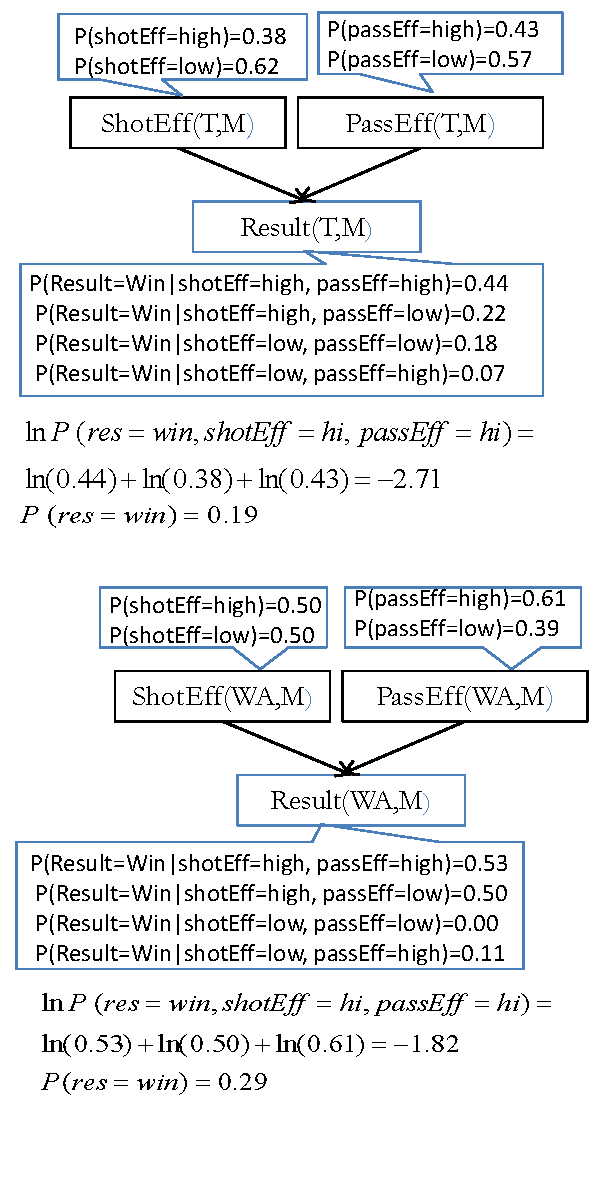
\includegraphics[width=0.4\textwidth] 
	{bnexamples-edited}
	\caption{Example of joint and marginal probabilities computed from a toy Bayesian network structure. The parameters were estimated from the  Premier League dataset. (Top): A class model Bayesian network $\model_{\class}$ for all teams with class parameters $\parameters_{\class}$. (Bottom): The same Bayesian network structure with object parameters $\parameters_{\object}$ learned for Wigan Athletics ($T = WA$). Our model-based methods outlier scores compare the data likelihood of the class parameters and the object parameters.
		%We show only the Markov blanket of the Results node to simplify. 
		\label{fig:bns}
	}
\end{figure}


\begin{figure}[t]
	\centering
	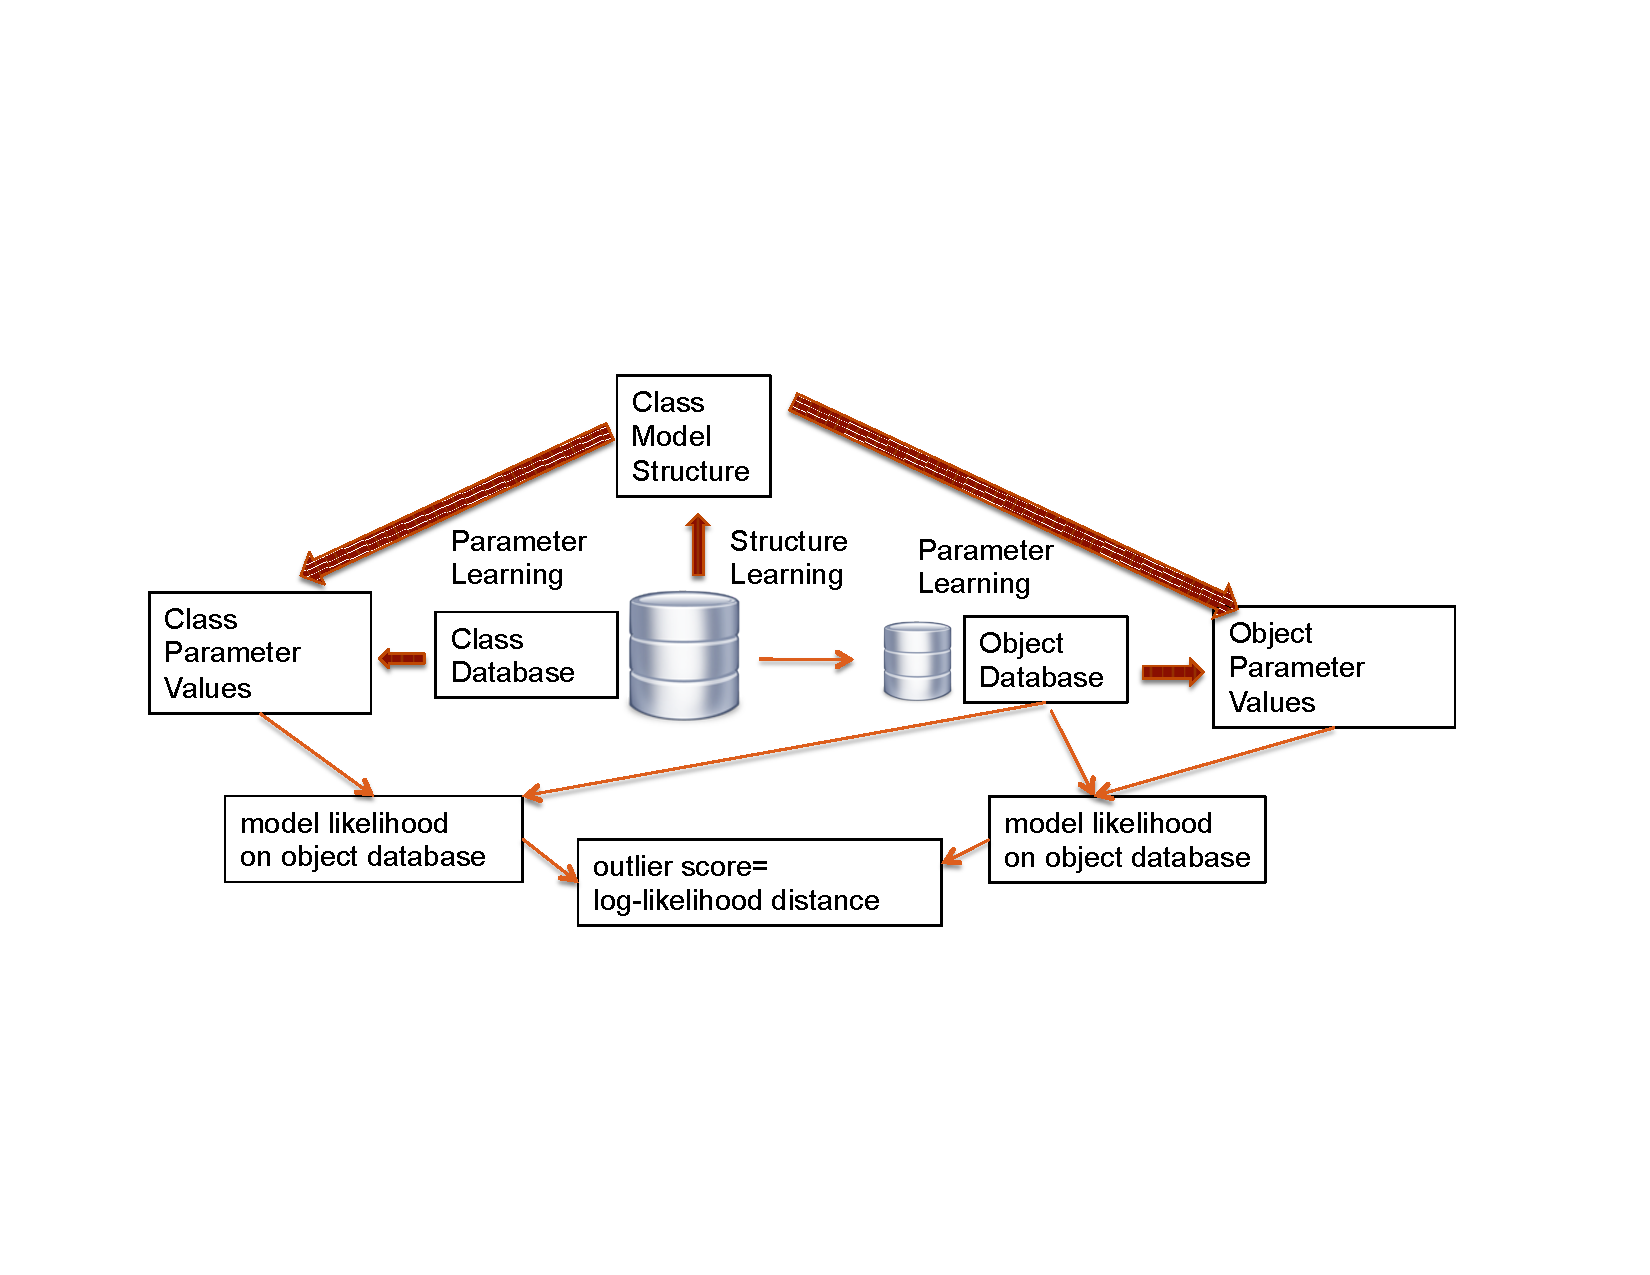
\includegraphics[width=0.4\textwidth]{flow.pdf}
	\caption{Computation of outlier score. 
		\label{fig:flow}}
\end{figure}
%				\begin{figure}
%				\centering
%				\resizebox{0.9\textwidth}{!}{
%				
%				\subfigure{
%				  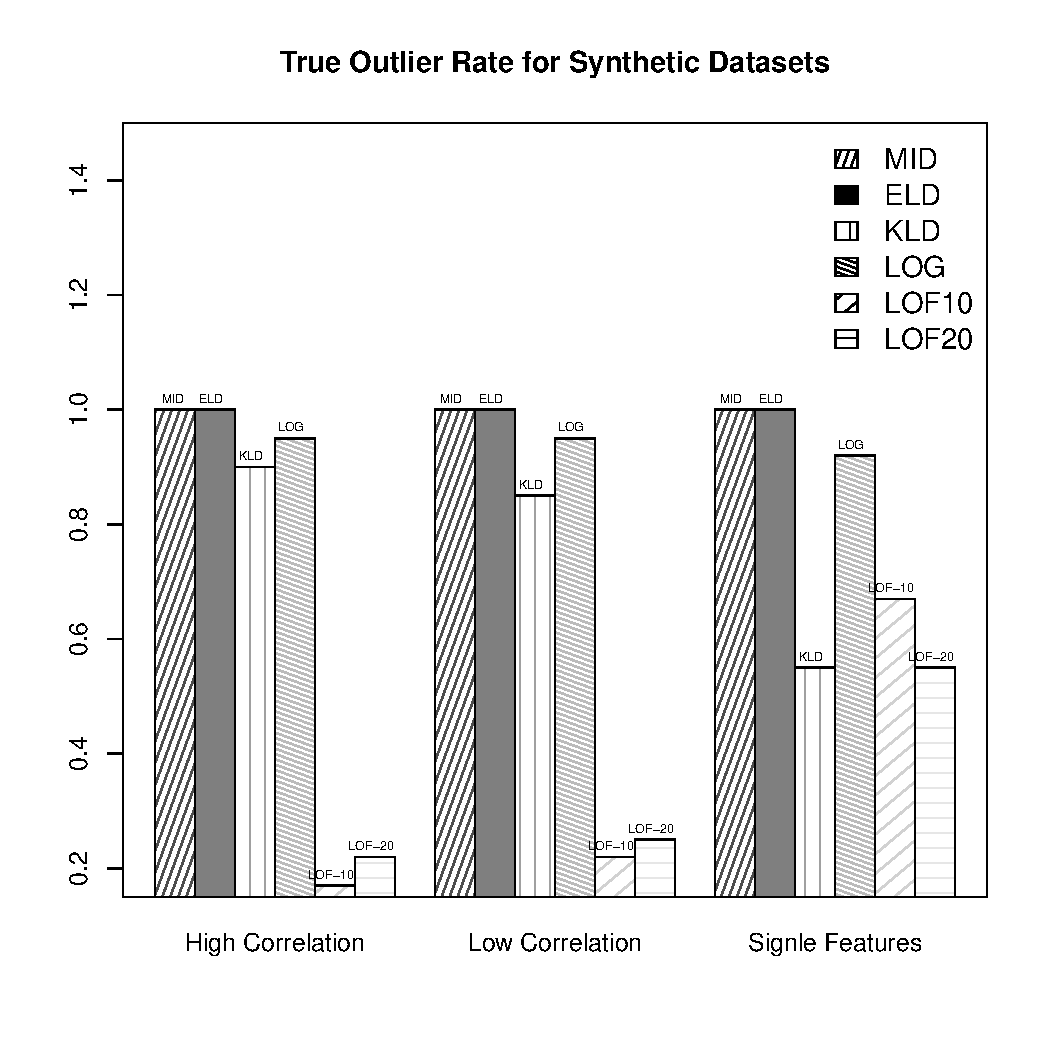
\includegraphics[height=70mm, width=70mm] {figures/TPR-Synthetic.pdf}
%				}
%				\subfigure{
%				  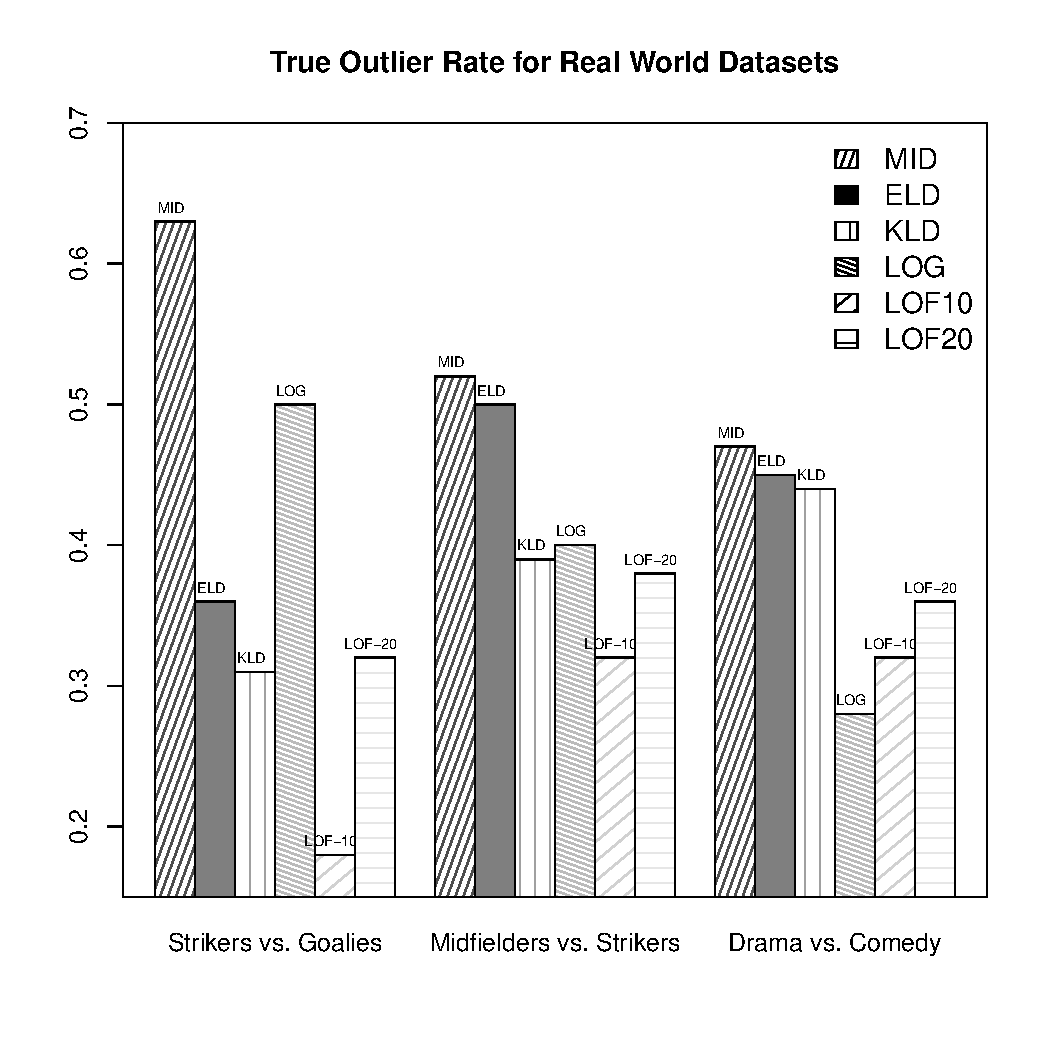
\includegraphics[height=70mm, width=70mm] {figures/TPR-All.pdf}
%				
%				 }
%				 }
%				
%				\caption{Comparison of Object Outlier Metrics}
%				\label{fig:synthetic}
%				\end{figure}
%				

%				\begin{figure}
%					\centering
%					\begin{subfigure}{0.4\textwidth}
%						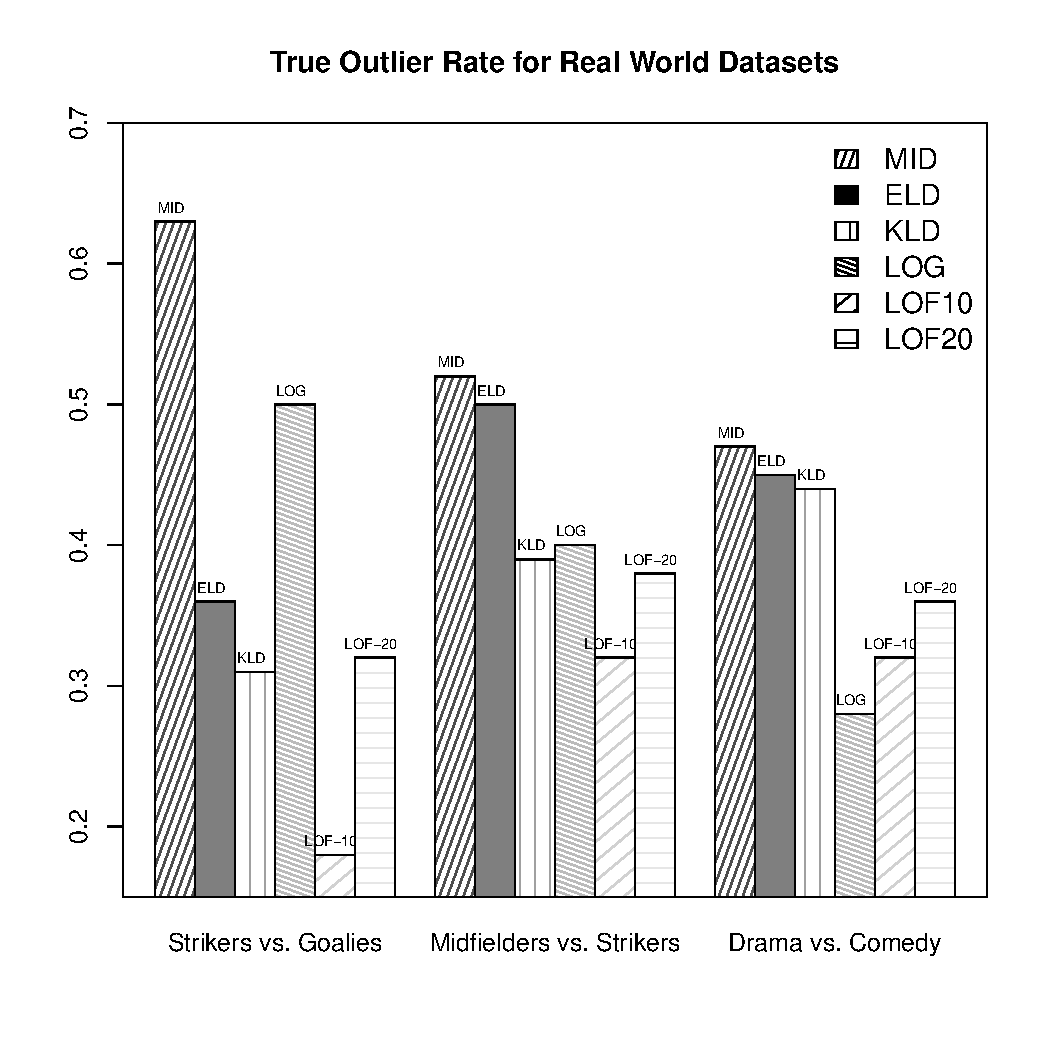
\includegraphics[width=1\linewidth]{figures/TPR-All.pdf}
%						\caption{}
%						\label{fig:Ng1} 
%					\end{subfigure}
%					
%					\begin{subfigure}{0.4\textwidth}
%						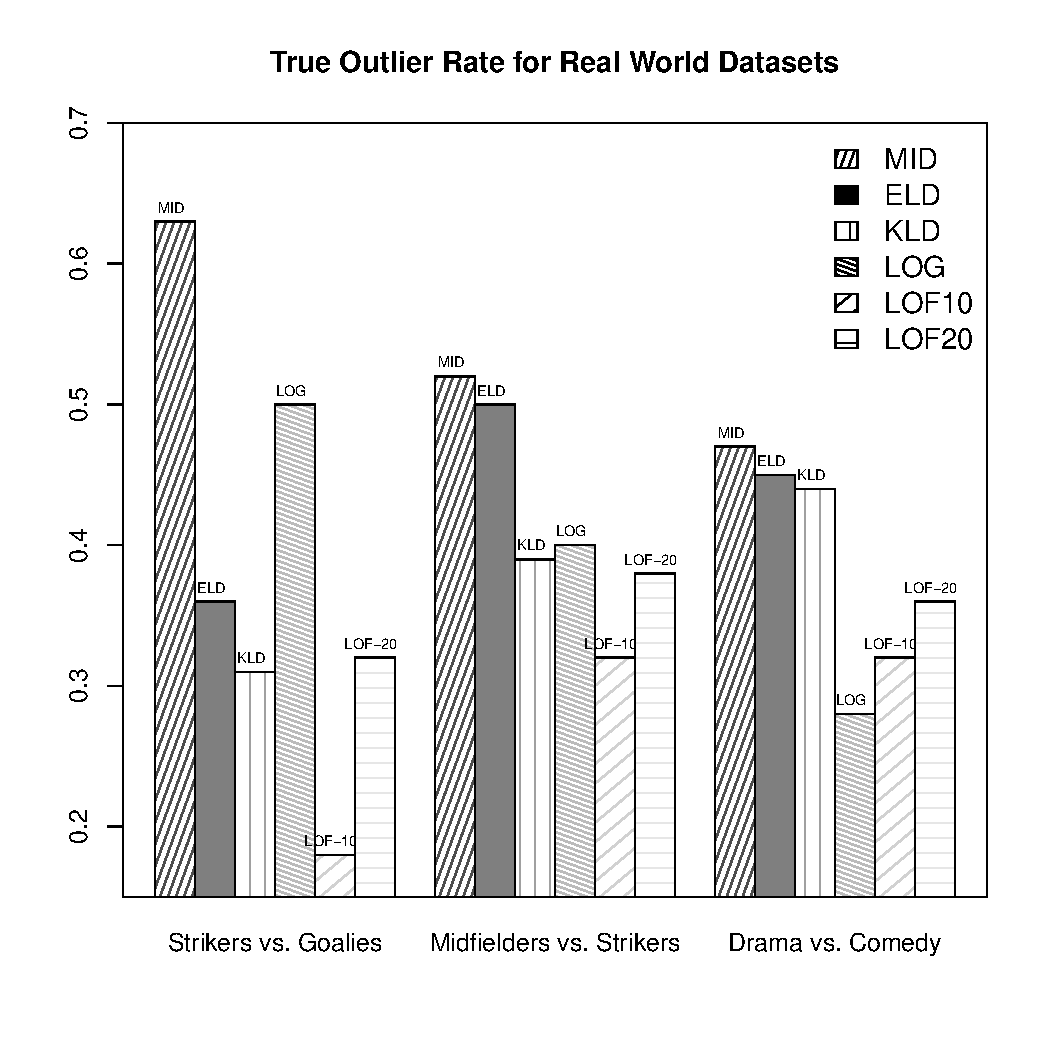
\includegraphics[width=1\linewidth]{figures/TPR-All.pdf}
%						\caption{}
%						\label{fig:Ng2}
%					\end{subfigure}
%					
%					\caption[Two numerical solutions]{(a) Numerical solutions for the small-time system 
%						with a constant-curvature body shape showing the scaled leading-order veritcal 
%						reaction force $N_0$ versus the scaled body mass $M$ for various values of $g$. 
%						Again, $I=M$ for definiteness and $A=0.7$. (b) As for (a) but over a wider range of 
%						values of $M,I$.}
%				\end{figure}

\subsection{Relational Data}




%We apply the learn-and-join algorithm (LAJ), which is the state-of-the-art Bayes net learning method for relational data. The LAJ algorithm takes as input a relational database and outputs a Bayes net using the functor notation due to Poole \cite{Poole2003}. We briefly review this notation.

%\paragraph{Functor Terms} 
We adopt a functor-based notation for combining logical and statistical concepts~\cite{Poole2003,Kimmig2014}.
A functor is a function or predicate symbol. Each functor has a set of values (constants) called the \textbf{domain} of the functor. The domain of a \textbf{predicate} is $\{\true,\false\}$. Predicates are usually written with uppercase Roman letters, other terms with lowercase letters.
A predicate of arity at least two is a \textbf{relationship} functor. Relationship functors specify which objects are linked. Other functors represent \textbf{features} or \textbf{attributes} of an object or a tuple of objects (i.e., of a relationship).
A \textbf{population} is a set of objects. 
A \textbf{term} is of the form $f(\term_{1},\ldots,\term_{k})$ where $\functor$ is a functor %(either a function symbol or a predicate symbol) 
and each $\term_{i}$ is a first-order variable or a constant denoting an object. A term is \textbf{ground} if it contains no first-order variables; otherwise it is a first-order term. In the context of a statistical model, we refer to first-order terms as \textbf{Parametrized Random Variables} (PRVs) \cite{Kimmig2014}. 
%A term whose range are the truth values $\{\true,\false\}$ is a \textbf{predicate}. 
%Predicates are usually written with uppercase Roman letters, other term with lowercase letters.
%The grounding concept represents moving from the population-level  to the object level. 
A \textbf{grounding} replaces each first-order variable in a term by a constant; the result is a ground term. A grounding may be applied simultaneously to a set of terms.  A relational database $\D$ specifies the values of all ground terms, which can be listed in data tables. 
%In machine learning terminology, the data tables are contingency tables that represent sufficient statistics or event counts.

Consider a joint assignment 
$P(\Features = \set{\nodevalue})$ of values to a set of PRVs $\Features$. The {\em grounding space} of the PRVs is the set of all possible grounding substitutions, each applied to all PRVs in $\Features$. The {\em count} of groundings that satisfy the assignment with respect to a database $\D$ is denoted by $\grounds_{\D}(\Features = \set{\nodevalue})$. The \textbf{database frequency} $P_{\D}(\Features = \set{\nodevalue})$ is the grounding count divided by the number of all possible groundings.
%, that is, the size of the grounding space.

\emph{Example.} \label{sec:example}
%
The Opta dataset represents information about premier league data %\cite{opta-original} 
(Sec.~\ref{sec:real-world-data}). 
%Using the functor notation, the data
%format can be represented as follows. 
The basic populations are teams, players, matches, with 
corresponding first-order variables $\team, \player, \match$. Table~\ref{table:data} specifies values for some ground terms. The first three column headers show first-order variables ranging over different populations. The remaining columns represent features. Table~\ref{table:counts} illustrates grounding counts. Counts are based on the 2011-2012 Premier League Season. We count only groundings $(\it{team},\it{match})$ such that $\it{team}$ plays in $\it{match}$. Each team, including Wigan Athletics, appears in 38 matches. The total number of team-match pairs is $38 \times 20 = 760$.

%Examples of terms include the following. 

%\begin{itemize}
%\item $\it{Appears\_Player}(\P,\M)$ indicates whether a player appeared in a match.
%\item $\it{Appears\_Team}(\T,\M)$ indicates whether a team played in a match.
%\item $\it{Team}(\P)$ returns the team of a player.
%\item $\it{Result}(\T,\M)$ denotes the result of a team in a match (win or lose).
%\item $\it{ShotEff}(\T,\M)$ denotes the shot efficiency of a team in a match (number of successful shots on target, per total number of shots).
%\item $\it{TimePlayed}(\P,\M)$ denotes the total time that a player played in a match.
%\end{itemize}


%\begin{table}[htbp]
%\caption{Examples of terms in the soccer dataset.}
%\centering
%\resizebox{0.5\textwidth}{!}{
%\begin{tabular}{|c|p{5cm}|}
%\hline
%Term&Meaning\\ \hline
%$\it{Appears\_Player}(\P,\M)$ & indicates whether a player appeared in a match.\\ \hline
%$\it{Appears\_Team}(\T,\M)$&indicates whether a team played in a match.\\ \hline
%$\it{Team}(\P)$& returns the team of a player.\\ \hline
%$\it{Result}(\T,\M)$ &denotes the result of a team in a match (win or lose).\\ \hline
%$\it{ShotEff}(\T,\M)$ &denotes the shot efficiency of a team in a match (number of successful shots on target, per total number of shots).\\ \hline
%$\it{TimePlayed}(\P,\M)$& denotes the total time that a player played in a match.\\ \hline
%\end{tabular}}
%\label{table:terms}
%\end{table}

\begin{table}[htbp]
	\caption{Sample Population Data Table (Soccer). \label{table:data}}
	\centering
	\resizebox{0.5\textwidth}{!}{
		\begin{tabular}{|c|c|l|c|c|c|c|}
			\hline
			\multicolumn{1}{|l|}{MatchId \match} &
			TeamId \team & PlayerId \player& \multicolumn{1}{l|}{First\_goal(\player,\match)} 
			& \multicolumn{1}{l|}{TimePlayed(\player,\match)} & 
			\multicolumn{1}{l|}{ShotEff(\team,\match)}&result(\team,\match) \\ \hline
			117 & WA & McCarthy & 0 & 90 & 0.53&\it{win}\\ \hline
			148 & WA & McCarthy & 0 & 85 & 0.57&\it{loss}\\ \hline
			15 & MC & Silva & 1 & 90 & 0.59&\it{win}\\ \hline
			\ldots& \ldots &\ldots&\ldots&\ldots&\ldots&\\
		\end{tabular}}
		\caption{Sample Object Data Table, for team $\team = \it{WA}$. \label{table:individual}}
		\resizebox{0.5\textwidth}{!}{
			\begin{tabular}{|c|c|l|c|c|c|c|}
				\hline
				\multicolumn{1}{|l|}{MatchId \match} &
				TeamId $\team = \it{WA}$ & PlayerId \player& \multicolumn{1}{l|}{First\_goal(\player,\match)} 
				& \multicolumn{1}{l|}{TimePlayed(\player,\match)} & 
				\multicolumn{1}{l|}{ShotEff(\it{WA},\match)}&result(\it{WA},\match) \\ \hline
				117 & WA & McCarthy & 0 & 90 & 0.53&\it{win}\\ \hline
				148 & WA & McCarthy & 0 & 85 & 0.57&\it{loss}\\ \hline
				\ldots& WA &\ldots&\ldots&\ldots&\ldots&\\
			\end{tabular}}
		\end{table}
		
		
		
		
		A novel aspect of our paper is that we learn model parameters for specific objects as well as for the entire population. 
		%To implement this, for each target object, we form 
		The appropriate \textbf{object data table} is formed from the population data table by restricting the relevant first-order variable to the target object. 
		For example, the object database for target Team $\it{Wigan Athletic}$, 
		forms a subtable of the data table of Table~\ref{table:data} that contains only rows where 
		TeamID = $\it{WA}$; see Table~\ref{table:individual}. In database terminology, an object database is like a view centered on the object. The object database is an individual-centered representation \cite{Flach1999a}.
		
		%\begin{table} 
		%	\captionsetup{singlelinecheck=off}
		%			\caption[.]{\label{table:counts}Example of Grounding Count and Frequency for the conjunction \begin{displaymath} \it{passEff(T,M)=hi}, shotEff(T,M)=high, Result(T,M)=1.\end{displaymath}}
		%			\centering
		%			\resizebox{0.5\textwidth}{!}{
		%				\begin{tabular}{|c|c|c|}
		%					\hline
		%					Database&Count or $\#_{D}(\Features = \set{\nodevalue})$&Frequency or $P_{D}(\Features = \set{\nodevalue})$\\\hline
		%					Population&76& $76/760=0.10$\\\hline
		%					Wigan Athletics&7&$7/38=0.18$\\\hline
		%		
		%					%Synthetic&40&280\\ \hline
		%				\end{tabular}}
		%			\end{table}
		\begin{table} 
			\caption{Example of Grounding Count and Frequency in Premier League Data, for the conjunction $\it{passEff(T,M)=hi}, shotEff(T,M)=hi, Result(T,M)=win$.\label{table:counts}}
			\centering
			\resizebox{0.5\textwidth}{!}{
				\begin{tabular}{|c|c|c|}
					\hline
					Database&Count or $\#_{D}(\Features = \set{\nodevalue})$&Frequency or $P_{D}(\Features = \set{\nodevalue})$\\\hline
					Population&76& $76/760=0.10$\\\hline
					Wigan Athletics&7&$7/38=0.18$\\\hline
					
					%Synthetic&40&280\\ \hline
				\end{tabular}}
			\end{table}
			
			%\begin{table} 
			%	\captionsetup{singlelinecheck=off}
			%			\caption[.]{\label{table:counts}Example of Grounding Count and Frequency for the conjunction \begin{displaymath} \it{passEff(T,M)=hi}, shotEff(T,M)=high, Result(T,M)=1.\end{displaymath} Counts are based on the 2011-2012 Premier League Season. We count only groundings $(\it{team},\it{match})$ such that $\it{team}$ plays in $\it{match}$. Each team, including Wigan Athletics, appears in 38 matches. The total number of team-match pairs is $38 \times 20 = 760$.
			%			\label{MetricComputation}}
			%			\centering
			%			\resizebox{0.5\textwidth}{!}{
			%				\begin{tabular}{|c|c|c|}
			%					\hline
			%					Database&Count or $\#_{D}(\Features = \set{\nodevalue})$&Frequency or $P_{D}(\Features = \set{\nodevalue})$\\\hline
			%					Population&76& $76/760=0.10$\\\hline
			%					Wigan Athletics&7&$7/38=0.18$\\\hline
			%		
			%					%Synthetic&40&280\\ \hline
			%				\end{tabular}}
			%				
			%			\end{table}
			
			%[Example of counts, frequencies]
			% For simplicity only, suppose that the only matches and players in the season are those shown in Table~\ref{table:data}. Then the attribute value $\it{First\_goals} = 0$ occurs with frequency $1/2$ in the object distribution $P_{\it{si}}$ for Silca. In the player class distribution $P_{\it{Player}}$, the attribute value $\it{First\_goals} = 0$ occurs with frequency $4/5$. So Silva is somewhat less likely to score no goal than a randomly selected player.
			\subsection{Bayesian Networks for Relational Data}
			
			A \textbf{Parametrized Bayesian Network Structure} (PBN) is a Bayesian network structure  whose nodes are PRVs. 
			%For most of the paper we refer to PBNs simply as Bayesian networks, and to PRVs simply as random variables. 
			%The learn-and-join algorithm is the state-of-the-art Bayes net learning method for relational data, based on model search in the lattice of relationship joins \cite{Schulte2012}. The LAJ algorithm takes as input a relational database and outputs a Parametrized Bayes net structure.
			%We review the algorithm very briefly; for further details please see \cite{Schulte2012}. 
			%The algorithm builds a Bayes net for an entire database by level-wise search through the {\em lattice of relationship chains.} This is the lattice of relationship sets that are connected by shared first-order variables.
			%%; see Figure~\ref{fig:lattice}.  
			%%We describe the fundamental ideas of the algorithm; for further details please see \cite{Schulte2012}. 
			%The user chooses a single-table Bayes net learner. The learner is applied to base population data tables. Then the learner is applied to data tables for relationship chains of size $s,s+1,\ldots$, with the constraint that the models for larger join tables inherit the absence or presence of learned edges from smaller join tables. 
			%
			The relationships and features in an object database define a set of nodes for Bayes net learning; see Figure~\ref{fig:bns}.
			% shows a sample PBN.
			
			
			%We use the following notation.
			
			%\begin{figure}[ht]
			%\centering
			%   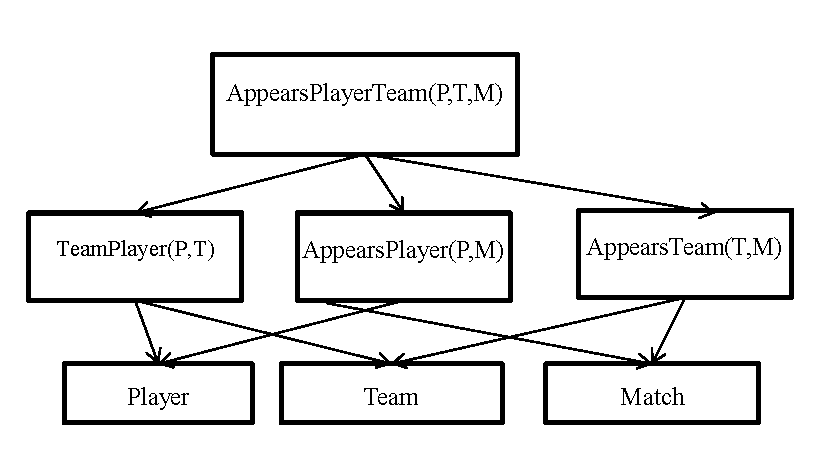
\includegraphics[width=0.3\textwidth] {lattice}
			% \caption{Lattice of Premier League dataset.
			% %We show only the Markov blanket of the Results node to simplify. 
			% \label{fig:lattice}}
			%\end{figure}
			
			
			
			
			%\begin{itemize}
			%\item $\D_{\population}$ is the database for the entire population; cf. Table~\ref{table:data}.
			%\item $\D_{\target}$ is the restriction of the input database to the target object; cf. Table~\ref{table:object}. 
			%\item $\M_{\population}$ is a model (e.g., Bayesian network) learned with $\D_{\population}$ as the input database; cf. Figure~\ref{fig:bns}(a).
			%\item $\M_{\target}$ is an object model (e.g., Bayesian network) learned with $\D_{\target}$ as the input database; cf. Figure~\ref{fig:bns}(b).
			%\end{itemize}
			%
			
			\subsubsection{Model Likelihood for Parametrized Bayesian Networks}
			
			A standard method for applying a generative model assumes that the generative model represents normal behavior since it was learned from the entire population. An object is deemed an outlier if the model assigns sufficiently low likelihood to generating its features \cite{Cansado2008}. This likelihood method is an important baseline for our investigation.
			%, so we define the likelihood function formally in this section. 
			%The other outlier scores we consider can be viewed as improved variants of the likelihood approach. 
			Defining a likelihood for relational data is more complicated than for i.i.d. data, because an object is characterized not only by a feature vector, but by an object  database.
			% that lists the object's links and the attributes of linked entities. 
			%For the model likelihood function $\lnlikelihood(\model,\D)$, where $\model$ denotes a Bayesian network, 
			We employ the relational pseudo log-likelihood \cite{Schulte2011}, which can be computed as follows for a given Bayesian network  and database.
			
			%\begin{eqnarray}
			%\lnlikelihood(\model,\D) =   \sum_{i=1}^{n}\sum_{j=1}^{\states_{i}} \sum_{\parents_{i}}\\ P_{\D}(\feature_{i} = \nodevalue_{ij},\parents_{i})\ln \parameter_{\model}(\feature_{i} = \nodevalue_{ij}|\parents_{i})  \nonumber
			%\end{eqnarray}
			
			\begin{equation} \label{eq:likelihood}
			\loglikelihood(\D,\model,\parameters) =   \sum_{i=1}^{n}\sum_{j=1}^{\states_{i}} \sum_{\parents_{i}}\P_{\D}(\nodevalue_{ij},\parents_{i})\ln \parameter(\nodevalue_{ij}|\parents_{i})  
			\end{equation}
			
			
			Equation~\eqref{eq:likelihood} represents the standard BN log-likelihood function for the object  data~\cite{Campos2006}, except that parent-child instantiation counts are standardized to be proportions \cite{Schulte2011}. The equation can be read as follows.
			
			\begin{enumerate}
				\item For each parent-child configuration, 
				use the conditional probability of the child given the parent.
				\item Multiply the logarithm of the conditional probability by the database frequency of the parent-child configuration. 
				%The instantiation proportion is the number of instantiating groundings, divided by the total number of possible instantiations.
				\item Sum this product over all parent-child configurations and all nodes. 
			\end{enumerate}
			
			%\begin{eqnarray}
			%\lnlikelihood&   \sum_{i=1}^{n}\sum_{j=1}^{\states_{i}} \sum_{\parents_{i}} P_{\D}(\feature_{i} = \nodevalue_{ij},\parents_{i})\ln \parameter_{\model}(\feature_{i} = \nodevalue_{ij}|\parents_{i})
			%\end{eqnarray}
			
			Schulte proves that the maximum of the pseudo-likelihood ~\eqref{eq:likelihood} is given by the empirical database frequencies \cite[Prop.3.1.]{Schulte2011}. In all our experiments we use these maximum likelihood parameter estimates.
			
			{\em Example.} The family configuration \begin{displaymath} \it{passEff(T,M)=hi}, shotEff(T,M)=hi, Result(T,M)=win\end{displaymath} contributes one term to the pseudo log-likelihood for the BN of Figure~\ref{fig:bns}. For the population database, this term is $0.1 \times \ln(0.44) =-0.08 $. For the  Wigan Athletics database, the term is $0.18 \times \ln(0.44) =-0.14 $. 
			%consider the parent-child configuration as shown in Figure~\ref{fig:bns}(b). Suppose that the data show that team $\it{WA}$ played 20 matches  in formation 1 with team shot efficiency at level 2 and won 12 of these. Then the maximum likelihood estimate of winning given the parent values is $12/20=0.6.$ The instantiation count is 10, so the instantiation proportion is $10/20 =0.5$. This parent-child configuration contributes $\ln 0.5 \cdot 0.6 = -0.415$ to the aggregate pseudo-likelihood. 
			
			%\section{Class and Object Distributions} 
			
			
			
			%\section{Overview} We describe the object-oriented data model and our approach to defining an object outlier score. In the object-oriented data model, complex objects are composed of simpler objects. This can be visualized as a tree. Objects are associated with attribute values. In this paper we assume that attributes take on discrete values, but this is not essential for our approach. 
			%Figure~\ref{fig:oobn} shows a typical object tree. Matches are complex objects containing a home team and an away team. The match result is a match attribute. Teams are complex objects comprising players. Some player attributes  depend on the context of the match. Players have a special attribute that specifies their class. Note that the same object can appear in different nodes (e.g., Van Persie). 
			%
			%\begin{figure*}[htbp]
			%	\centering
			%	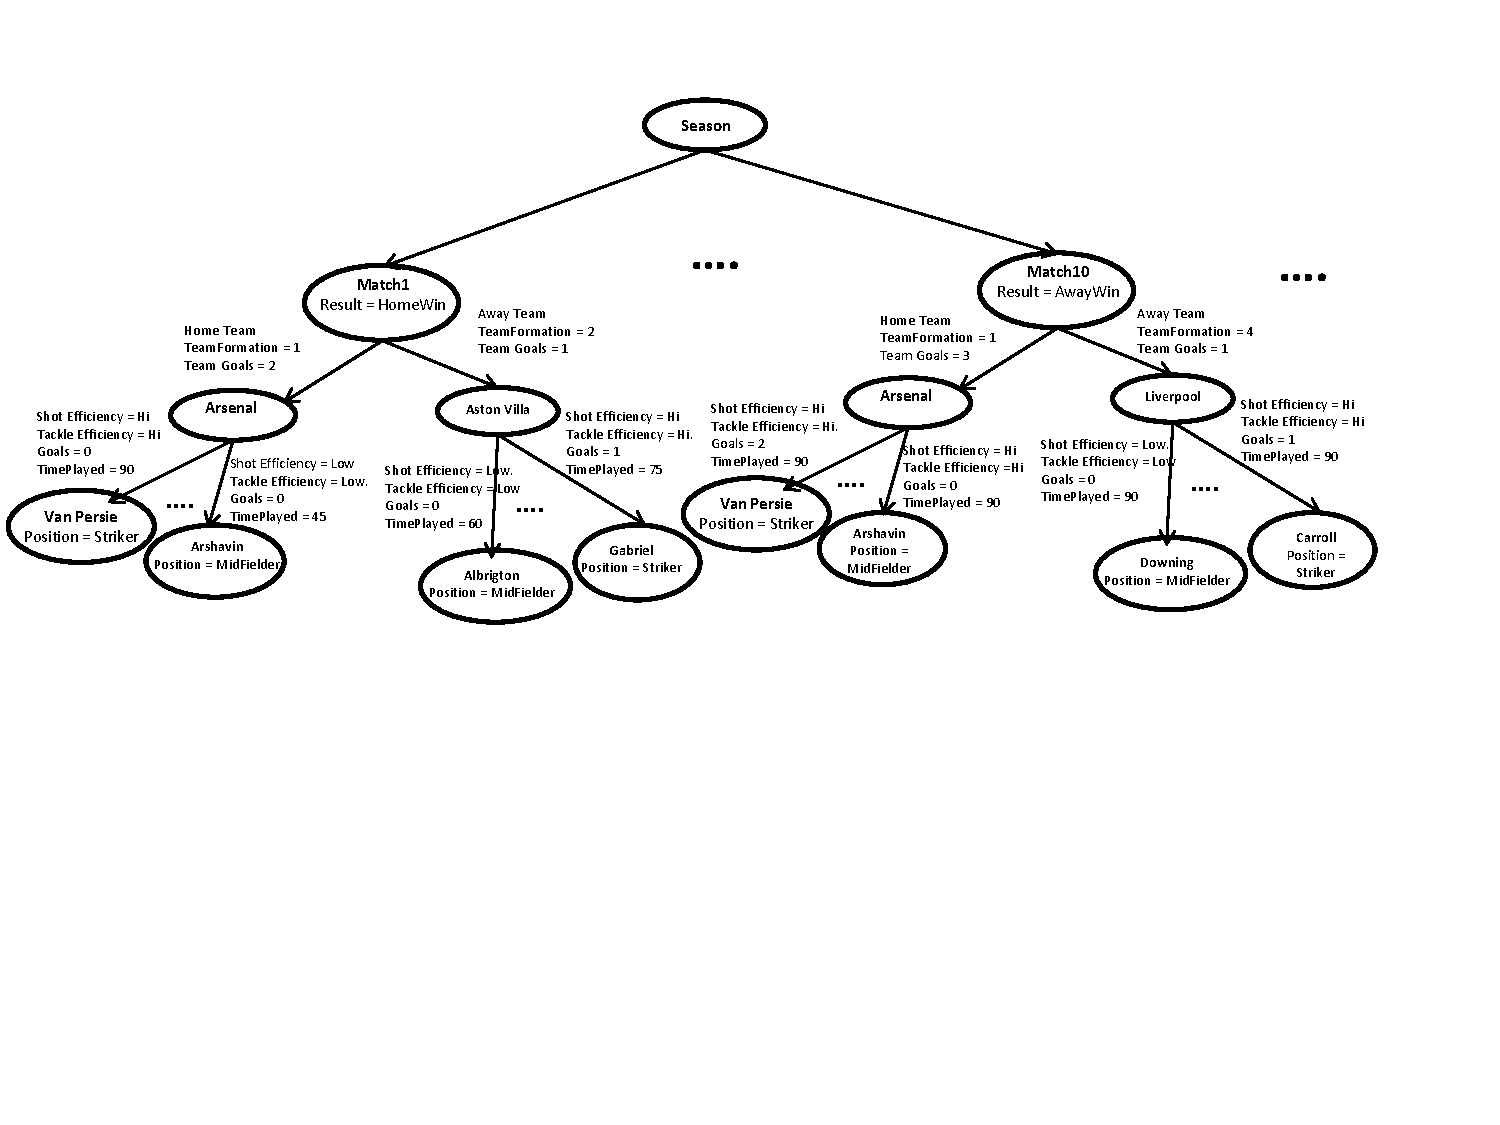
\includegraphics[width=1\textwidth]{SeasonGraph}
			%	\caption{An illustrative object tree. Nodes are labelled with object IDs and object attributes. A season is a complex object comprising matches. A match comprises a home team and an away team. Teams comprise players. Edges go to component objects.  Edge labels indicate the type of component relationship between the linked objects, and attributes associated with this  relationship. 
			%		\label{fig:oobn}}
			%\end{figure*}
			%
			%Our system employs the following steps for outlier detection, illustrated in Figure~\ref{fig:}. 
			%
			%\begin{enumerate}
			%	\item Define a set of path types in the object tree.
			%	\item For a given target object, there is a substructure that contains the other objects linked to the target by paths of the applicable types. We refer to this substructure as the {\em object profile}.
			%	\item For each attribute, the {\em object distribution} counts how many times the attribute occurred in the object's profile. 
			%	\item We define a novel distribution divergence that measures how much the target object's distribution differs from the average distribution of objects in the same class. This divergence is our outlier score.
			%\end{enumerate}
			%
			%In database terminology, an object profile is like a view centered on the object. For example, a query for computing the object profile for Arsenal would include the selection condition $\it{TeamID} = \it{Arsenal}$. Note that an object profile features both parts of the object as well as more complex objects of which it is a part. The object profile is individual-centered in the sense of \cite{Flach1999a}.
			%
			%\begin{figure}[htbp]
			%	\centering
			%	\resizebox{0.5\textwidth}{!}{
			%		\includegraphics%[width=0.3\textwidth] 
			%		{SystemOverView}
			%	}
			%	\caption{The components in our outlier detection system and the system flow. Aggregation is an alternative to our expected log-distance outlier score.
			%		\label{fig:flow}}
			%\end{figure}
			%
			%\section{Path Types}
			%A path in the tree connects two nodes, with {\em links in either direction}. For example, the object tree contains a path $\it{van Persie} \leftarrow \it{Arsenal} \leftarrow \it{Match1}$ that connects van Persie to the first match of the season. Every path specifies a set of attribute values for the objects and edges contained in the path. 
			%A \textbf{path type} is a set of paths with matching node types and matching edge types. For example, the path $\it{van Persie} \leftarrow \it{Arsenal} \leftarrow \it{Match10}$ is of the same type as the previous one.  For each attribute of a path type, and each value of the attribute, there is a count of the number of times that the attribute value occurs in a path of the type. These counts define the {\em path type distribution.} 
			%%Given a list of path types, we can combine (concatenate) their distributions into a attribute distribution for the list. 
			%%maybe use the term ``metapath''
			%
			%Assume that a list of path types have been fixed. The \textbf{object profile} contains all instances of a type of path that begin with the object. For each type of path, there is a distribution of attribute values over paths of that type in the object profile.
			%The \textbf{object distribution} $P_{\object}$ for object $\object$ combines (concatenates) the path distributions 
			%%over all attributes 
			%in the object profile. 
			%%In order words, it represents the distribution of attribute values over all paths that begin with the object.
			%%a node labelled with the object's ID.
			%The expression $P_{\Class}$ denotes the joint \textbf{class distribution} for the class of object $\object$. This is the joint probability associated with selecting an object uniformly at random from its class. Equivalently, the class distribution can be viewed as the  uniform mixture of object distributions:
			%
			%$$P_{\Class} \equiv \frac{1}{|\Class|} \sum_{\object \in \Class} P_{\object}.$$
			%
			%\paragraph{Example} Suppose we consider only paths of the type $\,$
			%$\it{Player} \leftarrow 
			%\it{Team} \leftarrow \it{Match}$. The attributes of this path type include $\it{Goals},\it{TeamGoals},\it{ShotEfficiency},\it{Result}$. For simplicity only, suppose that the only matches and players in the season are those shown in Figure~\ref{fig:oobn}. Then the attribute value $\it{Goals} = 0$ occurs with frequency $1/2$ in the object distribution $P_{\it{vP}}$ for van Persie. In the player class distribution $P_{\it{Player}}$, the attribute value $\it{Goals} = 0$ occurs with frequency $5/8$. So van Persie is somewhat less likely to score no goal than a randomly selected player.
			%
			%Since our outlier scores are based on the object profiles, they depend on a specification of relevant path types. One option would be to exhaustively include all possible path types. Another is to let a user specify path types of interest, for example all paths of length $k$. In our experiments we use machine learning methods that search the space of path types to find the paths that carry the strongest probabilistic associations between objects (see Section~\ref{sec:bnlearning}  below). 
			
			
			
			%\section{Log-Distance Object Outlier score} \label{sec:metrics}
			%%[There is no bound on the number of objects that a complex object may contain. ]
			%
			%[log distances. Motivation: additive, decomposed, closed form for computation. Relates to baseline methods. Distance not difference: avoid cancelling. Weight by frequency in object domain]
			%
			%Our approach defines an object-oriented outlier score as a {\em model comparison score} of the form 
			%$$\scorediff(\model_{\object},\model_{\Class},\profile_{\object}).$$ Here $\profile_{\object}$ denotes the probability distribution defined by the profile of the potential outlier object $\object$, the symbol $\model_{\object}$ denotes a model of the object profile, and $\model_{\Class}$ denotes a model that represents the normal behavior in the population, learned from the entire dataset. 
			%We use the following notation and definitions to define model comparison scores formally. %
			%%\subsection{Notation and Bayesian Networks}
			%Fix a set of attributes $\Features = \{\feature_{1},\ldots,\feature_{n}\}$. These are attributes of objects, which can and typically do belong to different classes. In statistical terms, each attribute defines a random variable. The possible values of $\feature_{i}$ are enumerated as $\{\nodevalue_{i1},\ldots,\nodevalue_{i\states_{i}}\}$. The notation $P(\feature_{i} = \x)\equiv P(\x)$ denotes the probability of attribute $\feature_{i}$ taking on value $\x$. We also use the vector notation $P(\Features = \set{x}) \equiv P(\set{x})$ to denote the joint probability of that each attribute $\feature_{i}$ takes on value $\set{x}_{i}$. 
\section{Likelihood-Distance Object Outlier score} \label{sec:metrics}

We introduce a novel model-based outlier score, that extends the log-likelihood, using the following notation.
\begin{itemize}
	\item $\D_{\Class}$ is the database for the entire class of objects; cf. Table~\ref{table:data}. This database defines the \textbf{class distribution} $P_{\Class} \equiv P_{\D_{\class}}$.
	\item $\D_{\object}$ is the restriction of the input database to the target object; cf. Table~\ref{table:individual}. This database defines the \textbf{object distribution} $P_{\object} \equiv P_{\D_{\object}}$.
	\item $\model_{\Class}$ is a model (e.g., Bayesian network) learned with $\D_{\population}$ as the input database; cf. Figure~\ref{fig:bns}(a).
	\item $\parameters_{\Class}$ resp. $\parameters_{\object}$ are parameters learned for $\model_{\Class}$ using $\D_{\class}$ resp. $\D_{\object}$ as the input database.
\end{itemize}

Figure~\ref{fig:flow} illustrates these concepts and the system flow for computing an outlier score. First, we learn a Bayesian network $\model_{\Class}$ for the entire population using a previous learning algorithm (see Section~\ref{sec:methods} below). We then evaluate {\em how well the class model fits the target object data.} For vectorial data, the  standard model fit metric %approach 
is the log-likelihood of the target {\em datapoint}. For relational data, the counterpart is the relational log-likelihood \eqref{eq:likelihood} of the target {\em database}:

\begin{equation} \label{eq:loglikelihood-score}
\loglikelihood(\D_{\object},\model_{\Class},\parameters_{\Class}).
\end{equation}



While this
%the log-likelihood~\eqref{eq:loglikelihood-score} 
is a good baseline outlier score, it can be improved by considering scores based on the likelihood ratio, or {\bf log-likelihood difference}:
%. The log-likelihood difference is defined by

\begin{equation} \label{eq:log-diff}
\lr(\D_{\object},\model_{\Class},\parameters_{\object}) \equiv \loglikelihood(\D_{\object},\model_{\Class},\parameters_{\object}) - \loglikelihood(\D_{\object},\model_{\Class},\parameters_{\Class}).
\end{equation}

The log-likelihood difference compares  how well the class-level parameters fit the object data, vs. how well the object parameters fit the object data. In terms of the conditional probability parameters, it measures how much the log-conditional probabilities in the class distribution differ from those in the object distribution. Note that this definition applies only for relational data where an individual is characterized by a substructure rather than a ``flat'' feature vector. Assuming maximum likelihood parameter estimation, $\lr$ is equivalent to the Kullback-Leibler divergence between the class-level and object-level parameters~\cite{Campos2006}. 
%
While the $\lr$ score provides more outlier information than the model log-likelihood, it can be improved further by two transformations as follows. (1) Decompose the joint probability into a single-feature component and a mutual information component. (2) Replace log-likelihood differences by log-likelihood distances. The resulting score is the \textbf{log-likelihood distance} ($\mid$), which is the main novel score we propose in this paper. Formally it is defined as follows for each feature $i$. The total score is the sum of feature-wise scores. Section~\ref{sec:divergence-examples} 
below provides example computations.
%In other words, we assume that model comparison scores are decomposable, which is the case for Bayesian networks. 
%\small
%\begin{equation} \label{eq:mid-bn}
%\begin{aligned}
%%\sum_{j=1}^{\states_{i} P_{\object}(\feature_{i} = \nodevalue_{ij}) \left|\ln \frac{P_{\object}(\feature_{i} = \nodevalue_{ij})}\right| + \\
%%\sum_{i=1}^{n} \sum_{j=1}^{\states_{i}}P_{\object}(\feature_{i}=\nodevalue_{ij}) \ln \frac{P_{\object}(\feature_{i} = \nodevalue_{ij})}{P_{\Class}(\feature_{i} = \nodevalue_{ij})} +\\
%\mid_{i} =\sum_{j=1}^{\states_{i}} P_{\object}(\feature_{i} = \nodevalue_{ij}) \left|\ln \frac{P_{\object}(\feature_{i} = \nodevalue_{ij})}{P_{\Class}(\feature_{i} = \nodevalue_{ij})}\right|+\\
%\sum_{j=1}^{\states_{i}} \sum_{\parents_{i}} 
%P_{\object}(\feature_{i} = \nodevalue_{ij},\parents_{i})\\
%\left|\ln \frac{P_{\object}(\feature_{i} = \nodevalue_{ij}|\parents_{i})}{P_{\object}(\feature_{i})=\nodevalue_{ij}} - \ln \frac{P_{\Class}(\feature_{i} = \nodevalue_{ij}|\parents_{i})}{P_{\Class}(\feature_{i})=\nodevalue_{ij}}\right|.
%\end{aligned}
%\end{equation}
%\normalsize

%\small
\begin{equation} \label{eq:log-dist}
\begin{array}{l}
%\sum_{j=1}^{\states_{i} P_{\object}(\feature_{i} = \nodevalue_{ij}) \left|\ln \frac{P_{\object}(\feature_{i} = \nodevalue_{ij})}\right| + \\
%\sum_{i=1}^{n} \sum_{j=1}^{\states_{i}}P_{\object}(\feature_{i}=\nodevalue_{ij}) \ln \frac{P_{\object}(\feature_{i} = \nodevalue_{ij})}{P_{\Class}(\feature_{i} = \nodevalue_{ij})} +\\
\mid_{i} =\sum_{j=1}^{\states_{i}} P_{\object}(\nodevalue_{ij}) \left|\ln \frac{\parameter_{\object}( \nodevalue_{ij})}{\parameter_{\Class}( \nodevalue_{ij})}\right|+\\
\sum_{j=1}^{\states_{i}} \sum_{\parents_{i}} 
P_{\object}( \nodevalue_{ij},\parents_{i})
\left|\ln \frac{\parameter_{\object}( \nodevalue_{ij}|\parents_{i})}{\parameter_{\object}(\nodevalue_{ij})} - \ln \frac{\parameter_{\Class}( \nodevalue_{ij}|\parents_{i})}{\parameter_{\Class}(\nodevalue_{ij})}\right|. \end{array}
\end{equation}
%\normalsize
%\paragraph{Motivation} 
%
%We note that for a fixed object distribution $P_{\object}$, the log-likelihood distance is a proper distance metric between the class-level and the object-level parameters. 
%The $\mid$ has two components. 
The first sum is the \textbf{single-feature} component, where each feature is considered independently of all others. It computes the expected log-distance with respect to  the singe feature value probabilities between the object and the class models. 
%For example, the single-feature sum for the feature ``Goal" of Van Persie is 5/8. 
%
The second $\mid$ sum is the \textbf{mutual information component}, based on the mutual information among all features. It computes the expected log-distance between the object and the class models with respect to the mutual information of feature value assignments.
%measures the expected distance in 
%%{\em multi-variate mutual information} 
%{\em association component} between the object and the class distributions. 
Intuitively, the first sum measures how the models differ if we treat each feature in isolation. The second sum measures how the models differ in terms of how strongly parent and child features are associated with each other. 
%A standard result in information theory states that a joint distribution can, without loss of information, be decomposed into a univariate distribution and the multi-variate mutual information  \cite{Witten2005}. Considering how the distributions differ in each of these two terms therefore involves no loss of information. 

%$\mid$ is not symmetric between the object and the class distribution because it weights sum terms by the joint probability in  the object distribution. The lack of symmetry is a desirable feature because to assess whether an object is an outlier, we want to weight most the events that occur more frequently with the object. 

\subsection{Motivation} 
%The motivation for using log-distances %rather than log-differences 
%is that some log-differences are positive, some negative, and cancel each other out when their sign differs. Since our goal is to assess the distinctness of an object, {\em we do not want differences to cancel out.} Fundamentally, averaging differences is appropriate when considering costs, payoffs or utilities, but not appropriate when assessing the distinctness of an object. 
%
The motivation for the mutual information decomposition is two-fold. 

\noindent
(1) {\em Interpretability}, which is very important for outlier detection. The single-feature components are easy to interpret since they involve no feature interactions. Each parent-child local factor is based on the average relevance of parent values for predicting the value of the child node, where relevance is measured by $\ln (\parameter(\nodevalue_{ij}|\parents_{i})/\parameter(\nodevalue_{ij}))$. This relevance term  is basically the same as the widely used lift measure \cite{Tuffery2011}, therefore an intuitively meaningful quantity. The $\mid$ score compares how relevant a given parent condition is in the object data with how relevant it is in the general class. 

\noindent
(2) {\em Avoiding cancellations.} Each term in the log-likelihood difference \eqref{eq:log-diff} decomposes into a relevance difference and a marginal difference: 

\begin{equation} \label{eq:decompose}
\ln \frac{\parameter_{\object}( \nodevalue_{ij}|\parents_{i})}{\parameter_{\Class}( \nodevalue_{ij}|\parents_{i})} = \ln \frac{\parameter_{\object}(\nodevalue_{ij}|\parents_{i})}{\parameter_{\object}(\nodevalue_{ij})} - \ln \frac{\parameter_{\Class}( \nodevalue_{ij}|\parents_{i})}{\parameter_{\Class}(\nodevalue_{ij})} + \ln \frac{\parameter_{\object}( \nodevalue_{ij})}{\parameter_{\Class}( \nodevalue_{ij})}.
\end{equation}

These differences can have different signs for different child-parent configurations and cancel each other out; see Table~\ref{table:Formula}. Taking distances as in Equation~\ref{eq:log-dist} avoids this undesirable cancellation. Since our goal is to assess the distinctness of an object, {\em we do not want differences to cancel out.} The general point is that averaging differences is appropriate when considering costs, or utilities, but not appropriate for assessing the distinctness of an object. For instance, the average of both vectors (0,0) and (1,-1) is 0, but their distance is not.



\subsection{Comparison Outlier Scores} Our lesion study compares our log-likelihood distance  $\mid$ score to baselines that are defined by omitting a component of $\mid$. In this section we define these scores.
%and provide a theoretical comparison. 
The scores increase in sophistication in the sense that they apply more transformations of the log-likelihood ratio. 
%Our empirical comparison below indicates that the 
More sophisticated scores provide more information about outliers.   
%defines the scores formally.  
Table~\ref{table:Formula} defines local feature scores; the total score is the sum of feature-wise scores. All metrics are defined such that {\em a higher score indicates a greater anomaly.} The metrics are as follows. 

\begin{description}
	\item[Feature Divergence $\fd$] is the first  component of the $\mid$ score. It considers each feature independently (no feature correlations).
	%							
	\item[Log-Likelihood Score \loglikelihood] is the standard model-based outlier detection score using data likelihood.
	\item[Log-Likelihood Difference \lr] is the log-likelihood difference~\eqref{eq:log-diff} between the class-level and object-level parameters. %(Equation). 
	\item[Log-Likelihood Difference with absolute value $|\lr|$] replaces differences in $\lr$ by distances.
	\item[Log-Likelihood Difference with decomposition $\lr^{+}$] applies a mutual information decomposition to $\lr$.
\end{description}



\begin{table}
	\caption{Baseline Outlier Scores for Bayesian Networks
		\label{table:Formula}}
	\resizebox{0.5\textwidth}{!}{
		\begin{tabular}{|l|l|} \hline
			Method & Formula\\
			\hline
			
			$\fd_{i}	$&	$\begin{array}{l}\sum_{i=1}^{n}\sum_{j=1}^{\states_{i}} P_{\object}( \nodevalue_{ij}) \left|\ln \frac{\parameter_{\object}( \nodevalue_{ij})}{\parameter_{\Class}( \nodevalue_{ij})}\right|\end{array}	$\\ \hline
			
			$-\loglikelihood_{i}$& $  \begin{array}{l} -\sum_{i=1}^{n}\sum_{j=1}^{\states_{i}} \sum_{\parents_{i}} P_{\object}( \nodevalue_{ij},\parents_{i})\ln \parameter_{\Class}( \nodevalue_{ij}|\parents_{i})\end{array}$ \\ \hline
			$\lr_{i}$&$\begin{array}{l}  \sum_{j=1}^{\states_{i}} \sum_{\parents_{i}} P_{\object}( \nodevalue_{ij},\parents_{i})\ln \frac{\theta_{\object}(  \nodevalue_{ij}|\parents_{i})}{\theta_{\Class}( \nodevalue_{ij}|\parents_{i})}.  \end{array}$\\	\hline
			$|\lr_{i}|$& $\begin{array}{l}  \sum_{j=1}^{\states_{i}} \sum_{\parents_{i}} P_{\object}( \nodevalue_{ij},\parents_{i})|\ln \frac{\theta_{\object}(\nodevalue_{ij}|\parents_{i})}{\theta_{\Class}( \nodevalue_{ij}|\parents_{i})}|. \end{array}$ \\	\hline
			$\lr_{i}^{+}$&$\begin{array}{l}  \sum_{j=1}^{\states_{i}} P_{\object}( \nodevalue_{ij}) \ln \frac{\parameter_{\object}( \nodevalue_{ij})}{\parameter_{\Class}( \nodevalue_{ij})}+
			\\ \sum_{j=1}^{\states_{i}} \sum_{\parents_{i}} 
			P_{\object}( \nodevalue_{ij},\parents_{i})
			\ln \frac{\theta_{\object}( \nodevalue_{ij}|\parents_{i})}{\parameter_{\object}(\nodevalue_{ij})} - \ln \frac{\theta_{\Class}( \nodevalue_{ij}|\parents_{i})}{\parameter_{\Class}(\nodevalue_{ij})}.  \end{array}$ \\ \hline
			
		\end{tabular} 
	}
\end{table}

\section{Examples} \label{sec:divergence-examples} 


We provide three simple examples with only two features that illustrate the computation of the outlier scores. They are designed so that outliers and normal objects are easy to distinguish, and so that it is easy to trace the behavior of an outlier score.
%The examples also illustrate the concepts of attribute and correlation outlier. 
The examples therefore serve as thought experiments that bring out the strengths and weaknesses of model-based outlier scores. 
Figure~\ref{fig:synthetic-bns} describes the BN representation of the examples. Table~\ref{table:example} provides the computation of the scores. For intuition, we can think of a soccer setting, where each match assigns a value to each attribute $F_i, i =  1,2$ for each player. 
Scores for the $F_{2}$ feature are computed conditional on $F_{1} = 1$. Expectation terms are computed first for $F_{2} = 1$, then $F_{2} = 0$. 

The single feature distributions are uniform, so the feature component $\mid_{1}$ 
is 0 for each node in both examples.
% 
The table illustrates the undesirable cancelling effects in $\lr$. In the high correlation scenario~\ref{fig:synthetic-bns}(a), the outlier object has a lower probability than the normal class distribution of $\it{Match\_Result} = 0$ given that $\it{Shot\_Efficiency} = 1$. Specifically, 0.5 vs. 0.9. The outlier object exhibits a higher probability $\it{Match\_Result} = 1$ than the normal class distribution, conditional on $\it{Shot\_Efficiency} = 1$; specifically, 0.5 vs. 0.1. In line 1, column 2 of Table~\ref{table:example}  the log-ratios $\ln(0.5/0.9)$ and $\ln(0.5/0.1)$ therefore have different signs. In the low correlation scenario~\ref{fig:synthetic-bns}(b), the cancelling occurs in the same way, but with the normal and outlier probabilities reversed. 
The cancelling effect is even stronger for attributes with more than two possible values.


\begin{table}[hbpt]
	\caption{Example Computation of different outlier scores.
		% for the examples.
		% of Figure~\ref{fig:synthetic-bns}(a),(b). 
	} 
	\label{table:example}
	
	%\captionsetup[table]{skip=10pt}
	
	\centering
	\resizebox{0.5\textwidth}{!}{
		\begin{tabular}{|c|p{3cm}|p{6cm}|l|}
			\hline
			Score&$F1=1$ Computation&$F2|F1=1$ Computation&Result\\ \hline
			$\lr$&\begin{tabular}{p{5cm}} $1/2 \ln(0.5/0.5)=0 $\end{tabular}&$1/4\ln(0.5/0.9)+ 1/4\ln(0.5/0.1)$&0.36\\ \hline
			%$ELD$&$1/2|\ln(0.5/0.5)|=0$&$1/4|\ln(0.5/0.9)|+1/4|\ln(0.5/0.1)|$&0.79\\ \hline
			$|\lr|$&$0$ (no parents)&\begin{tabular}{p{5cm}}$1/4 |\ln(0.5/0.5)-\ln(0.9/0.5)|+1/4 |\ln(0.5/0.5)-\ln(0.1/0.5)|$\end{tabular}&0.79\\ \hline
			$\fd$&$|\ln(0.5/0.5)|=0$&\begin{tabular}{p{5.5cm}}$1/2|\ln(0.5/0.5)| + 1/2|\ln(0.5/0.5)|$\end{tabular}&0\\ \hline
			$$\mid$$&$0+0$&$0.79+0$&0.79
			%$1/4(|\ln(0.9/0.5)-\ln(0.5/0.5)|+|\ln(0.1/0.5)-\ln(0.5/0.5)|+2|\ln(0.5/0.5)|)=0.54$
			\\ \hline
		\end{tabular}}
		%\centering
		\resizebox{0.5\textwidth}{!}{
			\begin{tabular}{p{8cm}}
				Table V(a): High Correlation Case, Figure~\ref{fig:synthetic-bns}(a).
				%: The scores for the object and class BNs of Figure~\ref{fig:synthetic-bns}(a).
				
			\end{tabular}}
			
			%
			\centering
			\resizebox{0.5\textwidth}{!}{
				\begin{tabular}{|l|p{3cm}|p{6cm}|l|}
					\hline
					Score&$F1=1$ Computation&$F2|F1=1$ Computation&Result\\ \hline
					$\lr$&$1/2\ln(0.5/0.5)=0$&$0.5 \cdot 0.9 \ln(0.9/0.5)+ 0.5 \cdot 0.1 \ln(0.1/0.5)$&0.26\\ \hline
					%$ELD$&$1/2|\ln(0.5/0.5)=0|$&$0.5 \cdot 0.9|\ln(0.9/0.5)|+0.5 \cdot 0.1|\ln(0.1/0.5)|$&0.50\\ \hline
					$|\lr|$&$0$ (no parents) &$0.5 \cdot 0.9 |\ln(0.9/0.5)-\ln(0.5/0.5)|+ 0.5 \cdot 0.1 |\ln(0.1/0.5)-\ln(0.5/0.5)| $&0.50\\ \hline
					$\fd$&$|\ln(0.5/0.5)|=0$&$1/2|\ln(0.5/0.5)| + 1/2|\ln(0.5/0.5)|$&0\\ \hline
					$\mid$&$0+0$&$0.5+0$&0.5\\ \hline
				\end{tabular}}
				\resizebox{0.5\textwidth}{!}{
					\begin{tabular}{p{8cm}}
						Table V(b): Low Correlation Case. Figure~\ref{fig:synthetic-bns}(b).
						%The scores for the object and class BNs of Figure~\ref{fig:synthetic-bns}(b). 
						
					\end{tabular}}
				\end{table}
				
				
				
				
				
				%The advantages of succinctness and interpretability obtain also for computing scores. We write $B_{\object}$ for a BN that represents the object distribution, and $B_{\Class}$ for a BN that represents the class distribution. Then $\lr$ can be decomposed as $\lr = \sum_{i =1} ^{n} \lr_{i}$, where $$\lr_{i} = \sum_{j=1}^{\states_{i}} \sum_{\parents_{i}} \ln \frac{P_{B_{\object}}(\feature_{i} = \nodevalue_{ij}|\parents_{i})}{P_{B_{\Class}}(\feature_{i} = \nodevalue_{ij}|\parents_{i})}$$ where $\parents_{i}$ indexes all possible parent value combinations for node $\feature_{i}$, and the $P_{B}$ terms denote the conditional probability parameters of the applicable Bayesian network. In words, we sum over all possible child-parent states, and compute the log-probability ratio of the object and class conditional probabilities. The Bayesian network decompositions for the other scores are as follows. We compute feature score as before directly from the class and object distributions, rather than the Bayesian networks, since it concerns only marginal single-feature probabilities. 
				
				%\begin{eqnarray*} 
				%%\tag{$\lr(P_{\object}||P_{\Class})$} 
				%\eld_{i} & = & \sum_{j=1}^{\states_{i}} \sum_{\parents_{i}} |\ln \frac{P_{B_{\object}}(\feature_{i} = \nodevalue_{ij}|\parents_{i})}{P_{B_{\Class}}(\feature_{i} = \nodevalue_{ij}|\parents_{i})}|\\
				%\jid_{i} & = & \sum_{j=1}^{\states_{i}} \sum_{\parents_{i}} |\ln \frac{P_{B_{\object}}(\feature_{i} = \nodevalue_{ij}|\parents_{i})}{P_{\object}(\feature_{i})=\nodevalue_{ij}} - \ln \frac{P_{B_{\Class}}(\feature_{i} = \nodevalue_{ij}|\parents_{i})}{P_{\Class}(\feature_{i})=\nodevalue_{ij}}|\\
				%\mid_{i} & = &
				%\label{eq:eld}
				%\end{eqnarray*}
				
				
				
				
				
				%The learning algorithms were executed with 64-bit Centos with 4GB RAM and an Intel Core i5-480 M processor. 
				
				
				
				%\subsection{Outlier Metrics Compared}
				
				%\begin{description} 
				%We evaluate the outlier scores $\mid,\eld,\lr$ described in Section~\ref{sec:divergences}. 
				%
				%We use two existing baseline methods. 
				
				%\paragraph{Likelihood Method.} 
				%The metric $\lnlikelihood$ is defined by the equation:
				
				%\begin{equation*} \label{eq:ll}
				%\lnlikelihood_{i} = \sum_{j=1}^{\states_{i}} \sum_{\parents_{i}} P_{\object}(\feature_{i} = \nodevalue_{ij},%\parents_{i})\ln P_{\Class}(\feature_{i} = \nodevalue_{ij}|\parents_{i})
				%\end{equation*}
				
				%The intuition behind this metric is that the class distribution Bayesian network represents normal behavior\cite%{riahi2013}. An object is deemed an outlier if  the class BN assigns sufficiently low likelihood to generating %its features. Using low model likelihood to identify outliers is a common application of Bayesian networks \cite%{Cansado2008a}.  The equation above represents the standard BN log-likelihood function for the object data, %except that parent-child instantiation counts are standardized to be proportions. 
				%This avoids giving exponentially more influence to features with more groundings \cite{Schulte2011}. 
				
				
				%\item[\mid] The outlier metric is the Mutual Information Distance defined in Equation \eqref{eq:mid}. 
				%
				%\item[\eld] The outlier metric is the Mutual Information Distance defined in Equation \eqref{eq:eld}. 
				%
				%\item[\lr] The outlier metric is the KL divergence between the generic and the individual feature distribution. 
				%
				%\item[\lnlikelihood]  The outlier metric is the standardized log-likelihood $\lnlikelihood$ of the generic Bayesian network applied to the individual feature distribution. 
				%\marginpar{define, ranks everything the same on BN example (b).}
				%\item[\lr] The outlier metric is the likelihood ratio metric $\lr$. The Bayesian network learning method for the target individual's network uses the LAJ algorithm.
				
				%\item[
				
				%\paragraph{Local Outlier Factor.}
				
				%The local outlier factor is a popular density-based outlier metric that has been used as a baseline in previous %studies \cite{Breunig2000}. The metric requires specifying the number of nearest neighbors $k$. The authors of %the $\lof$ method recommend choosing a value between 10 and 20; we use 10 and 20.
				%\end{description}
				
				%$\lof$ requires as input a flat data matrix where each individual is represented by a single feature vector. To %aggregate features of individuals across complex objects such as matches or ratings, we use the total feature %count. This is the approach of the inventors of $\lof$ for sports data \cite{Breunig2000}. For example, they %counted the total number of goals scored by a player in a season as a feature for outlier analysis. We used the %implementation of $\lof$ in $\it{Data mining with R(DMwR)}$ package in R.
				
				%\subsection{Performance Metric} To score each outlier metric against ground truth instances, we follow the %%%approach of \cite{Gao2010,Cansado2008a}: Given the ground truth that $r\%$ of instances are outliers, we sort the outlier scores in descending order, and take the top $r\%$ as the outliers indicated by the method. We then report the true positive rate (recall), or \textbf{true outlier rate} (TOR), and the true negative rate, or \textbf{true normal rate} (TNR). The TNR is thus the percentage of normal individuals with rank below the top $r\%$. In anomaly detection the true outlier rate is the most important metric \cite{Gao2010,Cansado2008a}.
				
				
				\section{Related Work}
				Outlier detection is a densely researched field, for a survey please see~\cite{aggarwal2013}.
				Figure~\ref{fig:novelty} provides a tree picture of where our method is situated with respect to other outlier detection methods and other data models. 
				%For an outlier detection survey please see~\cite{aggarwal2013}.
				%\cite{Hodge2004,aggarwal2013}. 
				Our method falls in the category of {\em unsupervised} statistical model-based approaches. To our knowledge, ours is the first model-based method tailored for object-relational data. Like other model-based approaches, it detects {\em global outliers.} Aggarwal \cite{aggarwal2013} defines a global outlier to be a data point that notably deviates from the rest of the population. We review relevant approaches from different data models, the most common atomic object model---where data is represented by vectors---and structured data models.\\
				
				% using the XML, SQL, and OLAP formats.
				%\vspace{-5mm}
				\textit{a) Attribute Vector Data Model:}
				%\footnote{\textbf{Sarah}: can you fix the silly d) for paragraph numbering?}By far most work on outlier detection considers atomic objects with flat feature vectors.
				By far most work on outlier detection considers atomic objects with flat feature vectors.
				%, or nonhierarchical structures like time series. 
				This leads to an impedance mismatch: 
				The required input format for these outlier detection methods is a single data matrix, not a structured dataset. For example, one cannot provide a relational database as input. This mismatch is not simply a question of choosing a file format, but instead reflects a different underlying data model: complex objects with both attributes and component objects vs. atomic objects with attributes only. 
				%
				It is possible to ``flatten'' structured data by converting it to unstructured feature vectors, for instance by using aggregate functions. 
				%Flattening incurs some loss of information but allows us to apply the many feature vector methods.
				%\cite{Elke2013}. 
				We evaluated the aggregation approach in this paper by applying three standard methods for outlier detection.
				%for three major approaches to outlier detection: distance-based, density-based, and subspace clustering. 
				%
				%Subspace clustering methods (e.g., \cite{Muller2012,Kriegel2009}) are similar to our work in the sense that they aim to decompose a complex data space. They find complex deviations that are noticeable only in a data subspace. A common approach is to discover datapoints that show unexpected deviations in similar subspaces. Our approach instead develops a joint measure of how dissimilar the target object profile distribution is to the class distribution over the entire data space. Given that object and class distributions are represented by an object-oriented Bayesian network \cite{Koller1997}, the network structure defines subspaces. The joint divergence measure {\em mathematically decomposes} into subspace measures that quantify how dissimilar the target object profile distribution is in the subspaces defined by the network, compared to the class distribution in the same subspace.
				
				Work on atomic contextual  outliers \cite{Tang2013} is like ours in that it considers the distinctness of a target individual from a reference class. A reference class is not specified for each object,
				%as a property of the object, 
				but is constructed as part of outlier detection. 
				Our work could be combined with a class discovery approach by providing a score of how informative the inferred classes are. 
				\begin{figure}
					\centering
					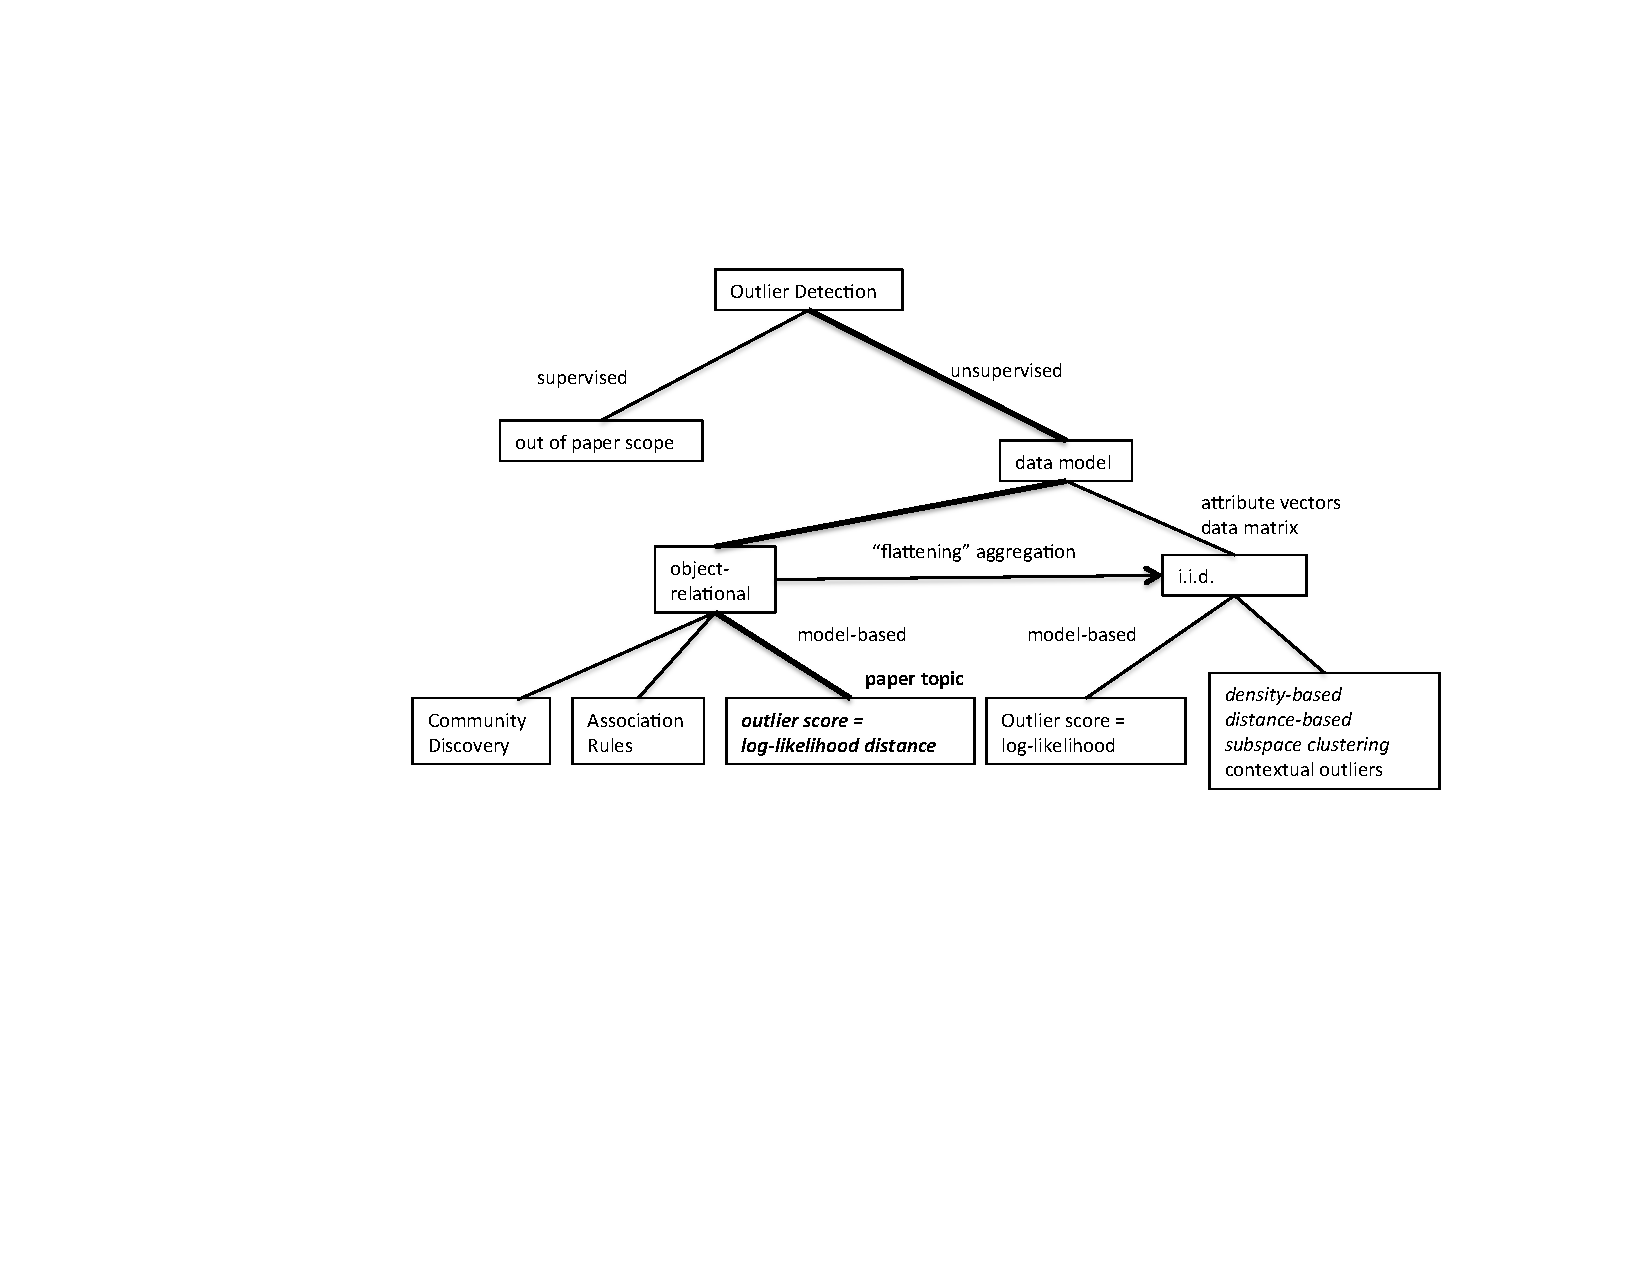
\includegraphics[width=0.5\textwidth] {NoveltyDiagram}
					\caption{A tree structure for related work on outlier detection for structured data. A path specifies an outlier detection problem, the leaves list major approaches to the problem. Approaches in italics appear in experiments.
						\label{fig:novelty}}
				\end{figure}
				%\vspace{-5mm}
				
				\textit{b) Structured Data Models:} We discuss related techniques in three types of structured data models: SQL (relational), XML (hierarchical), and OLAP (multi-dimensional). 
				
				For relational data, many outlier detection approaches aim to discover rules that represent the presence of anomalous associations for an individual or the absence of normal associations \cite{Maervoet2012,Gao2010}. The survey by \cite{Novak2009} unifies within a general rule search framework related tasks such as exception mining, which looks for associations that characterize unusual cases, subgroup mining, which looks for associations  characterizing important subgroups, and contrast space mining, which looks for differences between classes. Another rule-based approach uses Inductive Logic Programming techniques \cite{Angiulli2007}.
				%,Angiulli2009}.
				While local rules are informative, they are not based on a global statistical model and do not provide a single outlier score for each individual. 
				
				A latent variable approach in information networks ranks potential outliers in reference to the latent communities inferred by network analysis \cite{Gao2010}. Our model aggregates information from entities and links of different types, but does not assume that different communities have been identified. 
				
				
				Koh {\em et al.}~\cite{Koh2008} propose a method for hierarchical structures represented in XML document trees. Their aim is to identify feature outliers, not class outliers as in our work. Also, they use aggregate functions to convert the object hierarchy into feature vectors. Their outlier score is based on local correlations, and they do not construct a model.
				
				
				The multi-dimensional data model defines numeric measures for a set of dimensions. 
				%A seminal approach to exploring a multi-dimensional datacube was presented by Sarawagi {\em et al.}~\cite{Sarawagi1998}. 
				%The object and the multi-dimensional data models are similar in the respect that both objects and dimensions are ordered in a hierarchy. However, 
				The differences in the two data models mean that multi-dimensional outlier detection models~\cite{Sarawagi1998} do not carry over to object-relational outlier detection. (1) The object data model allows but does not require any numeric measures. In our datasets, all features are discrete. Nor do we assume that it is possible to aggregate numeric measures to summarize lower-level data at higher levels.  
				(2) In scoring a potential outlier object, our method considers other objects {\em both} below and above the target object in the component hierarchy. OLAP exploration methods consider only cells below or at the same level as the target cell. For example, in scoring a player, our method would consider features of the player's team.  
				Also, the $\mid$ outlier score of an object is not determined by the outlier scores of its components, in contrast to the approach of Sarawagi {\em et al.}.
				% They use values such as the most unusual cell that is below a target cell.
				(3) Our approach models a joint distribution over features, exploiting correlations among features. Most of the OLAP-based methods consider only a single numeric measure at a time, not a joint model.  
				
				
				
				\section{Experimental Design}
				%Details about our systems and algorithms that we use from previous work may be found in Section~\ref{sec:details}.  
				All the experiments were performed on a 64-bit Centos machine with 4GB RAM and an Intel Core i5-480 M processor. The likelihood-based outlier scores were computed with SQL queries using JDBC, JRE 1.7.0. and MySQL Server version 5.5.34.
				We describe the datasets used in our experiments.
				
				\subsection{Synthetic Datasets}
				
				We generated three synthetic datasets with normal and outlier players using the distributions represented in the three Bayesian networks of Figure~\ref{fig:synthetic-bns}. 
				%The features $F_{1}$ and $F_{2}$ represent two features of players. 
				Each player participates in 38 matches, similar to the real-world data. The main goal of designing synthetic experiments is to test the methods on  easy to detect outliers. Each match assigns a value to each feature $F_i, i =  1,2$ for each player. 
				\begin{description}
					\item\textbf{High Correlation} See Figure~\ref{fig:synthetic-bns}(a).
					\item\textbf{Low Correlation} See Figure~\ref{fig:synthetic-bns}(b).
					\item\textbf{Single features} See Figure~\ref{fig:synthetic-bns}(c).
				\end{description}
				
				
				
				
				
				%These datasets are designed so that outliers and normal objects are easy to distinguish, and so that it is easy to trace the behavior of an outlier score.
				
				%\begin{description}
				%\item[High Correlation]  See Figure~\ref{fig:synthetic-bns}(a).
				%\item[Low Correlation]  See Figure~\ref{fig:synthetic-bns}(b).
				%\item[Single attributes] See Figure~\ref{fig:synthetic-bns}(c).
				%\end{description}
				%
				We used the $\it{mlbench}$ package in $\it{R}$ to generate synthetic features in matches, following these distributions for 240 normal players and 40 outliers. We followed the real-world Opta data in terms of number of normal and outlier individuals. The scores are used to rank all 280 players. 
				\subsection{Real-World Datasets} \label{sec:real-world-data}
				Data tables are prepared from Opta data~\cite{opta-original} and IMDb~\cite{IMDb-original}. Our datasets and code are available on-line~\cite{bib:jbnsite}.
				\paragraph{Soccer Data} 
				The Opta data were released by Manchester City. 
				It lists box scores, that is, counts of all the ball actions within each game by each player, for the 2011-2012 season. 
				%The data consists of information about the actions of a single player in a given match 
				%from 2011 to 2012. 
				%Number of goals, passes, fouls, tackles, saves and blocks and also position 
				%assigned to a player in a match are examples of the information associated with each player. [list]
				%Information about the teams in a season, such as number of home wins, draws or away wins can be extracted by massaging the data. 
				%[The information can be visualized as a heterogeneous network that links players to teams, and teams to matches. ]
				For each player in a match, our data set contains eleven player features.
				% like $\it{TimePlayed}(\P,\M)$.
				For each team in a match, there are five features computed as player feature aggregates, as well as the team formation and the result (win, tie, loss). 
				There are two relationships, $\it{Appears\_Player}(\P,\M)$, $\it{Appears\_Team}(\T,\M)$. 
				%We store the data in a relational database, with a table for each base population and a table for each relationship.
				
				\paragraph{IMDB Data} 
				The Internet Movie Database (IMDB) is an on-line database of information related to films, television programs, and video games.
				The IMDB website offers a dataset containing information on cast, crew, titles, technical details and biographies into a set of compressed text files. 
				We preprocessed the data like \cite{Peralta2007} to obtain a database with seven tables: one for each population and one for the three relationships $\it{Rated}(\user,\movie)$, $\it{Directs}(\director,\movie)$, and $\it{ActsIn}(\actor,\movie)$.
				
				%				Table~\ref{table:Features} lists relationships and the number of features. 
				%				\begin{table}[htbp]
				%							\caption{Relationships and Example Features in Real-World Datasets.
				%								%For relationships please see text.
				%								\label{table:Features}}
				%					\centering
				%					\resizebox{0.3\textwidth}{!}{
				%						\begin{tabular}{|l|c|l|}
				%							\hline
				%							Path/Object Type & \#Attributes&Example\\ \hline
				%							\begin{tabular}{c}Player-Team-Match \end{tabular} & 11&ShotEff \\ \hline
				%							\begin{tabular}{c}Team-Match \end{tabular} & 7&TeamFormation \\ \hline\hline
				%							Actor & 2&Quality \\ \hline
				%							Director & 2&AvgRevenue\\ \hline
				%							Movie&5&Genre\\ \hline
				%							User& 2&Occupation\\ \hline
				%							User-Movie & 1&Rating \\\hline
				%							Actor-Movie & 1&Cast\_Position\\\hline
				%						\end{tabular}}
				%				
				%					\end{table}
				%\footnote{Commented table of relationships and features}
				%					\begin{LaTeXdescription}
				%						\item[Soccer Data]
				%						The Opta data were released by Manchester City. 
				%						It lists all the ball actions within each game by each player, for the 2011-2012 season.
				%						\item[IMDb Data]
				%						The Internet Movie Database (IMDb) is an online database of information related to films, television programs, and video games.
				%						The IMDb website offers a dataset containing information on cast, crew, titles, technical details and biographies in a set of compressed text files \cite{Peralta2007}.
				%					\end{LaTeXdescription}
				
				%\subsection{Outlier and Contrast Classes.}
				
				In real-world data, there is no ground truth about which objects are outliers. To address this issue, we employ a one-class design: we learn a model for the class distribution, with data from that class only. Then we rank all individuals from the normal class together with all objects from a contrast class treated as outliers, to test whether an outlier score recognizes objects from the contrast class as outliers.
				%		distinguishes objects from the normal class from objects in the contrast class. 
				Table~\ref{MetricComputation} shows the normal and contrast classes for three different datasets.  In-class outliers are possible, e.g. unusual strikers are still members of the striker class. Our case studies describe a few in-class outliers. In the soccer data, we considered only individuals who played more than 5 matches out of a maximum 38. 
				%The maximum number of matches played is 38.
				%
				%					In this design, we are only looking for the objects that are clearly deviating from the majority of the data. We are aware of the 
				
				%
				%\begin{description}
				%\item[Strikers vs. Goalies] The generic model is learned with match data from all 150 strikers. The outlier test cases are match data for all 22 goalies.
				%\item[Midfielder vs. Striker]  The generic model is learned with match data from all 172 midfielders. The outlier test cases are match data for 70 randomly selected strikers.
				%\item[Drama vs. Comedy] The generic model is learned with data for all 400 drama movies and 80 randomly selected comedy movies.
				%\end{description}
				%Figure~\ref{fig:synthetic} shows the true outlier rates for the different outlier metrics.  {\em On all datasets, the Mutual Information Score $\mid$ separates the normal class from the contrast class better than the other methods.} The same is true for the true negative rate; see supplementary file.
				%This rate reflects only the number of contrast objects that are ranked highly. Therefore we cannot expect a true outlier rate of 100\% because the normal class may also contain genuine outliers. If a metric correctly ranks these within-class outliers more highly than contrast class members, its TOR decreases. 
				% that are not in the contrast some strikers, may be genuine outliers within the striker class.
				
				\begin{table}
					\caption{Outlier/normal Objects in Real-World Datasets. }
					\label{MetricComputation}
					\centering
					\resizebox{0.8\textwidth}{!}{
						\begin{tabular}{|c|c|c|c|}
							\hline
							Normal&\#Normal&Outlier&\#Outlier\\\hline
							Striker & 153 & Goalie&22\\ \hline
							Midfielder & 155 & Striker&74\\ \hline
							Drama & 197 & Comedy&47\\ \hline
							%Synthetic&40&280\\ \hline
						\end{tabular}}
						
					\end{table}
					
					%						\subsection{Performance Score}
					%					 Our experiments provide empirical evidence that $\mid$ works better than other scores for object outlier detection.
					%						Our performance score for outlier rankings is the area under curve ($\auc$) of the well-established receiver operating characteristic $\roc$ curve.
					%						~\cite{Fawcett2006}. 
					%						This has been widely used to measure the performance of outlier ranking methods~\cite{Cansado2008, Muller2012}. The relationship between false positive rate (1- Specificity) and true positive rate (Sensitivity) is captured by the $\roc$ curve. Ideally, the best performance is achieved when we have the highest sensitivity and the highest specificity. 
					%					
					%						The maximum values for $\auc$ is 1.0 indicating a perfect ranking with 100\% sensitivity and 100\% specificity. In order to compute the $\auc$ value, we used the \textit{R} package \textit{ROCR}~\cite{RROCR2012}. Given a set of outlier scores, one for each object, this package returns an $\auc$ value. 
					%					
					
					\subsection{Methods Compared}
					\label{sec:methods}
					We compare two types of approaches, and within each approach several outlier detection methods. The first approach evaluates the likelihood-based outlier scores described in Section~\ref{sec:metrics}. For relational Bayesian network structure learning we utilize the previous learn-and-join algorithm (LAJ), which is
					a state-of-the-art BN structure learning method for relational data \cite{Schulte2012}. The LAJ algorithm employs an iterative deepening strategy, which can be described as as search through a lattice of table joins. For each table join, different BNs are learned and the learned edges are propagated from smaller to larger table joins. 	For a full description, complexity analysis, and learning time measurements, please see \cite{Schulte2012}. 	We used the implementation of the LAJ algorithm due to its creators \cite{bib:jbnsite}. 
					
					%						probabilistic scores applied directly to the  data structured as an object tree. 
					
					The second approach first ``flattens" the structured data into a matrix of feature vectors, then applies standard matrix-based outlier detection methods. We refer to such methods as \textbf{aggregation-based}
					%Flattening the object data allows applying the rich set of matrix-based outlier detection methods ``as is" 
					(cf. Figures~\ref{fig:novelty}). For example, this was the approach taken by Breunig {\em et al.} for identifying anomalous players in sports data \cite{Breunig2000}. Following their paper, for each continuous feature in the object data, we use the average over its values, and for each discrete feature, we use the occurrence count of each feature value in the object data. Aggregation 
					tends to lose information about correlations.
					%\cite{DavidJensen2002}. 
					Our experiments address the empirical question of whether this loss of information affects outlier detection. 
					%The advantage to the aggregation approach is that after aggregating to preprocess the data, any matrix-based outlier detection method can be applied; see Figure~\ref{fig:flow}. 
					We evaluated three standard matrix-based outlier detection methods: Density-based $\lof$~\cite{Breunig2000}, distance-based $\knn$~\cite{Ramaswamy2000} and subspace analysis $\outrank$~\cite{Muller2012}.
					%\footnote{commented descriptions of these methods }. 
					These represent common, fundamental  approaches for vectorial data. 
					%	Subspace analysis is especially relevant to our study because 
					Like $\mid$, subspace analysis is sensitive to correlations among features. 
					% Our experiments applied $\outrank$ with two subspace clustering models, \textit{PRO-CLUS} \cite{Muller2012} and \textit{DISH} \cite{Kriegel2007}.  
					We used the available implementation of all three data matrix methods from the state of the art data mining software \textit{ELKI} \cite{Elke2013}. We used \textit{PRO-CLUS} as the clustering function for $\outrank$, recommended by~\cite{Muller2012}.
					
					
					%	\subsubsection{Structured Data Methods}
					
					%						These include the $\mid$ and $\lr$ scores 
					%						that we introduced in Section~\ref{sec:metrics}. In addition, we apply the following two scores.
					%						
					%						
					%						
					%						 Including it as a baseline provides a lesion study for how important it is to consider the mutual information among attributes.
					%						Low model likelihood is a common score for using Bayesian networks to identify outliers \cite{Cansado2008}. The intuition behind the $\lnlikelihood$ score is that the class distribution Bayesian network represents normal behavior~\cite{riahi2013}. Low model likelihood therefore indicates anomalous objects. This is a common score for using Bayesian networks to identify outliers \cite{Cansado2008}.
					%An object is deemed an outlier if  the class BN assigns sufficiently low likelihood to generating its attributes.  
					%						The equation above represents the standard BN log-likelihood function for the object profile data, except that parent-child instantiation counts are standardized to be proportions \cite{Schulte2012}. 						
					%\subsubsection{Aggregation-based Matrix Methods}
					
					%%Standard outlier detection methods  require as input a flat data matrix where each individual is represented by a single attributes vector. To aggregate attributes of individuals across complex objects such as matches and ratings, we use the total attribute count. This is the approach that the inventors of $\lof$ \cite{Breunig2000} applied to sports data. For example they counted the total number of goals scored by a player in a season as a attribute for outlier analysis. 
					%						
					%For example, in the soccer dataset there is a correlation between ``shot efficiency" and ``dribble efficiency" of a striker and that correlation is a key feature to identify strikers from other class. However when we use the averages of these attributes,
					%%, by averaging over all the values of continuous attributes and counting the number of occurrences of different states of discrete attributes in all the player's matches, 
					%the correlation no longer exists. 
					% for comparison with $\mid$.
					%assume that the observations comprise independent data points that can be represented in a matrix. Since 
					%
					%Then, we study performance of \textit{MID} metric in comparison with:
					%\begin{description}
					%\item[$\lof$] is a density-based method originally presented in~\cite{Breunig2000} as a measure to quantify the outlier-ness of the data points relative to regions of different densities. Therefore, the score is defined based on local density instead of the nearest neighbor distance. In the simple words, $\lof$ compares the density of area around an object to the densities of the areas of the surrounding objects. However, $\lof$ defines density as the inverse of the average of the smoothed reachability distances in a neighborhood and this definition is not the precise definition of density in terms of number of data points within a specific region. $\lof$ is only sensitive to the density of the area and  ignore the orientation and the shape of the area.
					%\item[$\outrank$] is a subspace outlier ranking technique that employs the subspace analysis to identify the degree of outlierness. It compares clustered regions in different subspace and derive the outlierness score for each object. In this work we used $\outrank$ with two subspace clustering models \textit{PRO-CLUS} \cite{Muller2009} and \textit{DISH} \cite{Kriegel2007} (as suggested in~\cite{Muller2012} \textit{PRO-CLUS} is the best clustering function for their approach).
					%\item[$\knn$] is a well-known distanced-based outlier ranking method that is based on the distance of a point from its $k^{th}$ nearest neighbor and rank each object on the basis of its $k^{th}$ nearest neighbor. \cite{Ramaswamy2000}.
					%\end{description}
					
					%						\begin{LaTeXdescription}
					%							\item[$\lof$] is a standard density-based method~\cite{Breunig2000}.
					%							%It quantify the outlier-ness of the data points relative to regions of different densities. Therefore, the score is defined based on local density instead of the nearest neighbor distance. In the simple words, 
					%							$\lof$ compares the density of area around an object to the densities of the areas of the surrounding objects. 
					%							%However, $\lof$ defines density as the inverse of the average of the smoothed reachability distances in a neighborhood and this definition is not the precise definition of density in terms of number of data points within a specific region. $\lof$ is only sensitive to the density of the area and  ignore the orientation and the shape of the area.
					%							\item[$\knn$] is a well-known distanced-based outlier ranking method that assigns a score to each data point on the basis of distance of the point from its $k^{th}$ nearest neighbor ($D^k$) and  declare the top $n$ points as outliers~\cite{Ramaswamy2000}. 
					%							%They introduce a {\em partition-based} algorithm to set a upper bound and lower bound on $D^k$ to identify the partitions that cannot contain the top $n$ outliers and prune them in order to limit the search space. % \textbf{Sarah:more precise please}
					%							\item[$\outrank$] employs subspace analysis to measure the degree of outlierness. It compares clusters in different subspace to derive an outlier score for each object \cite{Muller2012}. \end{LaTeXdescription}
					
					%						Density and distance based methods are two fundamental approaches to outlier detection represented in our study by $\lof$ and $\knn$. Subspace analysis is a popular approach too, and relevant to our study because $\mid$ is sensitive to correlations among features as well. 
					
					
					\section{Empirical Results}
					
					We present results regarding computational feasibility, 
					%$\auc$ 
					predictive performance, and case studies.
					
					\subsubsection{Computational Cost of the $\mid$ Score.}
					%						
					%						Table~\ref{table:Number of Parameters} shows that the Bayesian network representation provides a highly compact summary of the target class distribution: the number of probabilities that need to be evaluated for computing the probabilistic scores decreases by a factor of 
					%						%\textbf{Sarah:fix dash}
					%						$10^{4}$\--$10^{5}$ depending on the dataset. 
					%						
					Table~\ref{table:LearningTime} shows that the computation of the $\mid$ value for a given target object is feasible. On average, it takes a quarter of a minute for each soccer player, and one minute for each movie. This includes the time for parameter learning from the object database.
					Learning the class model BN takes longer, but needs to be done only once for the entire object class. 
					{\em The BN model 
						%						is crucial for computational feasibility because it 
						provides a crucial %compact 
						low-dimensional representation of the 
						%joint 
						distribution information in the data.} Table~\ref{table:Number of Parameters} compares the number of terms required to compute the $\mid$ score in the BN representation to the number of terms in an unfactored representation with one parameter for each joint probability.
					
					\begin{table}[htbp]
						\centering
						\begin{subtable}
							%\caption{Time for computing the $\mid$ metric. This includes the time for Bayes Net structure learning.\label{table:LearningTime}}
							\centering
							\caption{Time (min) for computing the $\mid$ score. 
								%This includes the time for Bayes Net structure learning.
								\label{table:LearningTime}}
							\resizebox{0.8\textwidth}{!}{
								\begin{tabular}{|c|l|l|} \hline
									Dataset& Class Model
									%    \begin{tabular}{c} Class \\Terms (min)\end{tabular}   & 
									%    \begin{tabular}{c} Object \\Terms (min)\end{tabular}   
									& Average per Object  \\ \hline
									Strikers vs. Goalies&4.14&0.25\\ \hline
									Midfielder vs. Goalies &4.02&0.25 \\ \hline
									Drama vs. Comedy &8.30&1.00\\ \hline
								\end{tabular} 
							}
							
						\end{subtable}
						
						\begin{subtable}
							%\caption{The Bayesian network representation helps to decrease the number of terms that represent the class and object distributions. 
							%For relationships please see text.
							%\label{table:Number of Parameters}}
							\centering
							\caption{The Bayesian network representation decreases the number of terms required for computing the $\mid$ score.
								%that represent the class and object distributions.
								\label{table:Number of Parameters}}
							\resizebox{0.8\textwidth}{!}{
								\begin{tabular}{|c|l|l|}
									\hline
									Dataset & \begin{tabular}{c} \#Terms \\Using BN\end{tabular}  & \begin{tabular}{c} \#Terms \\ without Using BN
									\end{tabular}\\ \hline
									Strikers vs. Goalies & 1,430&114,633,792\\ \hline
									Midfielders vs. Goalies & 1,376&43,670,016\\ \hline
									Drama vs. Comedy & 50,802&215,040,000\\ \hline
								\end{tabular}
							}
							
						\end{subtable}
						
					\end{table}
					
					\subsubsection{Detection Accuracy} We follow the evaluation design of~\cite{Gao2010} and 
					make each baseline methods detect the same percentage of  objects as outliers:
					% as that of the ground-truths. To achieve this, we 
					Sort the outlier scores obtained by the three baseline methods in descending order, and take the top $r$ percent as outliers. Then we use \textbf{precision}, a.k.a. \textbf{true positive rate} as the evaluation metric which is the percentage of correct ones in the set of outliers identified by the algorithm. As in~\cite{Gao2010}, we set the percentages of outlier to be 1\% and 5\%. In the one-class design, precision measures how many members of the outlier class were correctly recognized. We also report some AUC measurements \cite{aggarwal2013}, which aggregate precision values at different percentage cutoffs.\footnote{Our $\mid$ score performs the best also with other metrics such as recall, to a similar degree; we omit the details due to space constraints.} %\textbf{Sarah: I'd love to have the plots of all points here.}
					
					
					\paragraph{Likelihood-Based Methods} 
					
					
					Table~\ref{table:Method Comparison} shows the $\auc$ values for each probabilistic ranking. Our $\mid$ score achieves the top score on each dataset. On the synthetic data, $\mid$ and $|\lr|$ are the only scores with 100\% precision at 1\% and 5\%. This confirms the value of using distances rather than differences. 
					%						However, the AUC score shows that $\mid$ retains perfect detection with different percentage cutoffs, but $|\lr|$ ranks some normal objects higher than actual outliers. 
					While it ought to be easy to distinguish the outliers, Table~\ref{table:Metric Comparison} shows that {\em $\mid$  is the only score that achieves perfect detection}, that is AUC = 1.0.
					
					%\footnote{\textbf{Sarah}: in the table LR is perfect as well. That's because we only look at precision, right?} 
					%For this reason, in Table~\ref{table:Method Comparison} we compare only the performance of $\mid$ to the previous data matrix methods.
					%						\begin{table}
					%							\begin{subtable}
					%								
					%								\centering
					%									\caption{$\auc$ of $\mid$ vs. other probabilistic scores. 
					%										%For relationships please see text.
					%										\label{table:Metric Comparison}}
					%								\resizebox{0.5\textwidth}{!}{
					%									
					%									\begin{tabular}{|l|l|l|l|l|}
					%										\hline
					%										Dataset & \mid &\lr &\fd&\lnlikelihood\\ \hline
					%										
					%										Synthetic Data-High Correlation & \textbf{1.00}&0.95&0.88&0.98 \\ \hline
					%										Synthetic Data-Low Correlation & \textbf{1.00}&0.95&0.35&0.95 \\ \hline
					%										Synthetic Data-Single Feature & \textbf{1.00}&0.89&0.79&0.98 \\ \hline
					%										Real Data-Strikers vs. Goalies & \textbf{0.89} &0.61&0.83& 0.65\\ \hline
					%										Real Data-Midfielders vs. Strikers &\textbf{0.66} &0.64 &0.52&0.64 \\ \hline
					%										Real Data-Drama vs. Comedy & \textbf{0.70} &0.65&0.61&0.63 \\ \hline
					%									\end{tabular}}
					%								
					%								\end{subtable}
					%								
					%								\begin{subtable}
					%									
					%									\centering
					%										\caption{$\auc$ of $\mid$ vs. aggregation-based Outlier Ranking Methods. 
					%											%For relationships please see text.
					%											\label{table:Method Comparison} 
					%										}
					%									\resizebox{0.5\textwidth}{!}{
					%										\begin{tabular}{|l|c|c|c|c|c|}
					%											\hline
					%											Dataset & $\mid$ &$\lof$&\begin{tabular}{c}$\outrank$\\(ProClus)\end{tabular}&\begin{tabular}{c}$\outrank$\\(DISH)\end{tabular}&\begin{tabular}{c}\it{KNN}\\\it{Outlier}\end{tabular}\\ \hline
					%											
					%											High Correlation & \textbf{1.00}&0.87&0.73&0.95&0.92 \\ \hline
					%											Low  Correlation & \textbf{1.00}&0.53&0.33&0.32&0.45 \\ \hline
					%											Single Feature & \textbf{1.00}&0.58&1.00&0.96&0.95\\ \hline
					%											Strikers vs. Goalies & \textbf{0.89} &0.68&0.89&0.53&0.75 \\ \hline
					%											Midfielders vs. Strikers &\textbf{0.66} &0.53 &0.54&0.49&0.55 \\ \hline
					%											Drama vs. Comedy & \textbf{0.70} &0.53&0.56&0.42&0.61 \\ \hline
					%										\end{tabular}}
					%									
					%									\end{subtable}
					%								\end{table}
					%											\begin{table}
					%									
					%															\caption{Precision of $\mid$ compare to other baseline scores in different datasets
					%																\label{table:CaseStudy}}
					%															\resizebox{0.5\textwidth}{!}{	
					%															\begin{tabular}{|l|c|c|c|c|c|c|c|c|}\hline
					%																	Dataset&\multicolumn{5}{|c|}{Structured-based models }&\multicolumn{3}{|c|}{Aggregation-based models}\\
					%																	\hline
					%																 &\mid&$|KLD|$&\lr&\fd&\lnlikelihood&\lof&$\outrank$	&\knn\\
					%																	\hline
					%																	High-Correlation &\textbf{1.00}&\textbf{1.00}&0.85&0.65&0.95&0.22&0.50&0.65\\
					%																	\hline	
					%																	Low-Correlation&\textbf{1.00}&\textbf{1.00}&0.90&0.25&0.95&0.25&0.10&0.10\\
					%																	\hline
					%																	Single-Feature&\textbf{1.00}&\textbf{1.00}&0.55&0.62&0.92&0.55&1.00&0.67\\\hline
					%																	Striker-Goali&\textbf{0.63}&0.36&0.31&0.58&0.40&0.32&0.50&0.52\\\hline
					%																	Midfielder-Striker&\textbf{0.52}&0.50&0.39&0.44&0.50&0.38&0.48&0.35\\\hline
					%																	Drama-Comedy&\textbf{0.47}&0.45&0.44&0.40&0.28&0.36&0.17&0.20\\\hline
					%																\end{tabular}	}		
					%																	
					%												\end{table}
					
					\begin{table}
						\caption{Precision of outlier scores in different datasets.
							\label{table:Method Comparison}}
						\resizebox{1\textwidth}{!}{	
							\begin{tabular}{|l|c|c|c|c|c|c|c|c|c|}\hline
								Dataset& percentage&\multicolumn{5}{|c|}{Model-based models }&\multicolumn{3}{|c|}{Aggregation-based models}\\
								\hline
								& &\mid&$|\lr|$&\lr&\fd&\loglikelihood&\lof&$\outrank$	&\knn\\
								\hline
								\multirow{2}{*}{High-Correlation}& 1\%& \textbf{1.00}& \textbf{1.00}& 0.73& 0.47& 0.91& 0.11& 0.53& 0.48\\
								&5\%&\textbf{1.00}&\textbf{1.00}&0.85&0.65&0.95&0.22&0.50&0.65\\\hline			
																										    	 \multirow{2}{*}{Low-Correlation}& 1\%& \textbf{1.00}& \textbf{1.00}& 0.87& 0.14& 0.93& 0.10& 0.00& 0.06\\
								&5\%&\textbf{1.00}&\textbf{1.00}&0.90&0.25&0.95&0.25&0.10&0.14\\
								\hline
								\multirow{2}{*}{Single-Feature}& 1\%& \textbf{1.00}& \textbf{1.00}& 0.39& 0.53& 0.81& 0.46& \textbf{1.00}& 0.51\\
								&5\%&\textbf{1.00}&\textbf{1.00}&0.55&0.62&0.92&0.55&\textbf{1.00}&0.54\\
								\hline    
								\multirow{2}{*}{Striker-Goalie}& 5\%& \textbf{0.57}& 0.27& 0.22& 0.51& 0.36& 0.19& 0.47& 0.42\\
								&15\%&\textbf{0.63}&0.36&0.31&0.58&0.40&0.32&0.50&0.52\\
								\hline    
								\multirow{2}{*}{Midfielder-Striker}& 1\%&\textbf{ 0.49}& 0.42& 0.25& 0.41& 0.46& 0.29& 0.44& 0.16\\
								&5\%&\textbf{0.52}&0.48&0.39&0.44&0.50&0.38&0.48&0.35\\
								\hline  													\multirow{2}{*}{Drama-Comedy}&1\%& \textbf{0.44}& 0.38& 0.39& 0.15& 0.22& 0.29& 0.07& 0.014\\
								&5\%&\textbf{0.47}&0.45&0.44&0.40&0.28&0.36&0.17&0.20\\
								\hline     
							\end{tabular}}		
							
						\end{table}
						
						%						\begin{table}
						%							\centering
						%								\caption{\textit{AUC} of $\mid$ vs. $|LR|$. 
						%									%For relationships please see text.
						%									\label{table:Metric Comparison}}
						%							\resizebox{0.3\textwidth}{!}{
						%								\begin{tabular}{|l|l|l|}\hline
						%									Dataset & \mid &$|\lr|$\\ \hline
						%									Synthetic Data-High Correlation & \textbf{1.00}&0.95 \\ \hline
						%									Synthetic Data-Low Correlation & \textbf{1.00}&0.95 \\ \hline
						%									Synthetic Data-Single Feature & \textbf{1.00}&0.89 \\ \hline
						%%									Real Data-Strikers vs. Goalies & \textbf{0.89} &0.61\\ \hline
						%%									Real Data-Midfielders vs. Strikers &\textbf{0.66} &0.64 \\ \hline
						%%									Real Data-Drama vs. Comedy & \textbf{0.70} &0.65 \\ \hline
						%								\end{tabular}}
						%							
						%							\end{table}
						%					\begin{table}
						%						\centering
						%						\caption{\textit{AUC} of $\mid$ vs. $|LR|$. 
						%							%For relationships please see text.
						%							\label{table:Metric Comparison}}
						%						\resizebox{0.5\textwidth}{!}{
						%							\begin{tabular}{|l|l|l|l|l|l|l|}\hline
						%								Score & high-Cor. &Low-Cor.&Single-Fe.&Striker&Midfielder&Drama\\ \hline
						%								 \mid&1.00&1.00&1.00&0.89&0.66&0.70\\\hline
						%								$|\lr|$&0.95&0.95&0.89&0.61&0.64&0.65\\\hline
						%							%	Synthetic Data-High Correlation & \textbf{1.00}&0.95 \\ \hline
						%							%	Synthetic Data-Low Correlation & \textbf{1.00}&0.95 \\ \hline
						%							%	Synthetic Data-Single Feature & \textbf{1.00}&0.89 \\ \hline
						%								%									Real Data-Strikers vs. Goalies & \textbf{0.89} &0.61\\ \hline
						%								%									Real Data-Midfielders vs. Strikers &\textbf{0.66} &0.64 \\ \hline
						%								%									Real Data-Drama vs. Comedy & \textbf{0.70} &0.65 \\ \hline
						%							\end{tabular}}
						%							
						%						\end{table}
						\begin{table}
							\centering
							\caption{\textit{AUC} of $\mid$ vs. $|LR|$. 
								%For relationships please see text.
								\label{table:Metric Comparison}}
							\resizebox{1\textwidth}{!}{
								\begin{tabular}{|l|l|l|l|l|l|l|}\hline
									Score & High-Cor. &Low-Cor.&Single-F.&Striker&Midfielder&Drama\\ \hline
									\mid&1.00&1.00&1.00&0.89&0.66&0.70\\\hline
									$|\lr|$&0.95&0.95&0.89&0.61&0.64&0.65\\\hline
									%	Synthetic Data-High Correlation & \textbf{1.00}&0.95 \\ \hline
									%	Synthetic Data-Low Correlation & \textbf{1.00}&0.95 \\ \hline
									%	Synthetic Data-Single Feature & \textbf{1.00}&0.89 \\ \hline
									%									Real Data-Strikers vs. Goalies & \textbf{0.89} &0.61\\ \hline
									%									Real Data-Midfielders vs. Strikers &\textbf{0.66} &0.64 \\ \hline
									%									Real Data-Drama vs. Comedy & \textbf{0.70} &0.65 \\ \hline
								\end{tabular}}
								
							\end{table}
							\paragraph{Aggregation-Based Methods vs. \mid} 
							Table~\ref{table:Method Comparison} shows the precision values for aggregation-based methods compared to $\mid$. {\em Our $\mid$ score outperforms all aggregation-based methods on all datasets}, except for a tie with $\outrank$(ProClus) on the relatively easy problem of distinguishing strikers from goalies.
							%								Comparing tables~\ref{table:Metric Comparison} and~\ref{table:Method Comparison} shows that t
							The performances of aggregation-based methods are most like that of the probabilistic score $\fd$, which does not consider the
							correlation among the features. This finding reflects the fact that aggregation tends to lose information about correlations.
							% \cite{DavidJensen2002}. 
							The aggregation-based methods achieve their highest performance on the Strikers vs. Goalies dataset. In this dataset action count features such as ShotsOnTarget, ShotEfficiency point to strikers and the feature SavesMade points to goalies. Therefore, outliers in this dataset are easy to find by considering features in isolation.
							%\\
							%\\
							%Based on the results shown in table ~\ref{table:Method Comparison}, the easiest dataset is Single Features, as most of the methods are successful in detecting outliers in that dataset. The low correlation dataset seems to be the most challenging one. 
							%The results of $\knn$ seem to be closest to $\mid$ in most datasets. 
							
							%The $\roc$ curve in Figure~\ref{fig:ROC} shows the performance of $\mid$ and $\knn$ which indicates that $\mid$ always reaches a higher true positive rate earlier that $\knn$.
							%\textbf{Sarah: both graph and table?}
							%Show the running time in a table. Explain that thats one of the weakness of $\mid$ compare to the others. But since the its performance is much higher than the compatitors it is worth the waiting!
							
							%
							%
							%
							%Strikers vs. goalies dataset is very similar to synthetic dataset, single feature in a sense that outlier and normal classes in both datasets contain single features that have distinct and very different distributions independent of the other attributes. In Strikers vs. Goalies attributes such as ShotsOnTarget or ShotEfficiency are valid only if the object is a member of Striker class and SavesMade only belongs to Goalie Class. Therefore, outliers in this dataset are also very easy to find even by applying the aggregation-based methods.  
							
							
							
							%\begin{figure*}
							%\centering
							%\resizebox{0.9\textwidth}{!}{
							
							%\subfigure{
							%  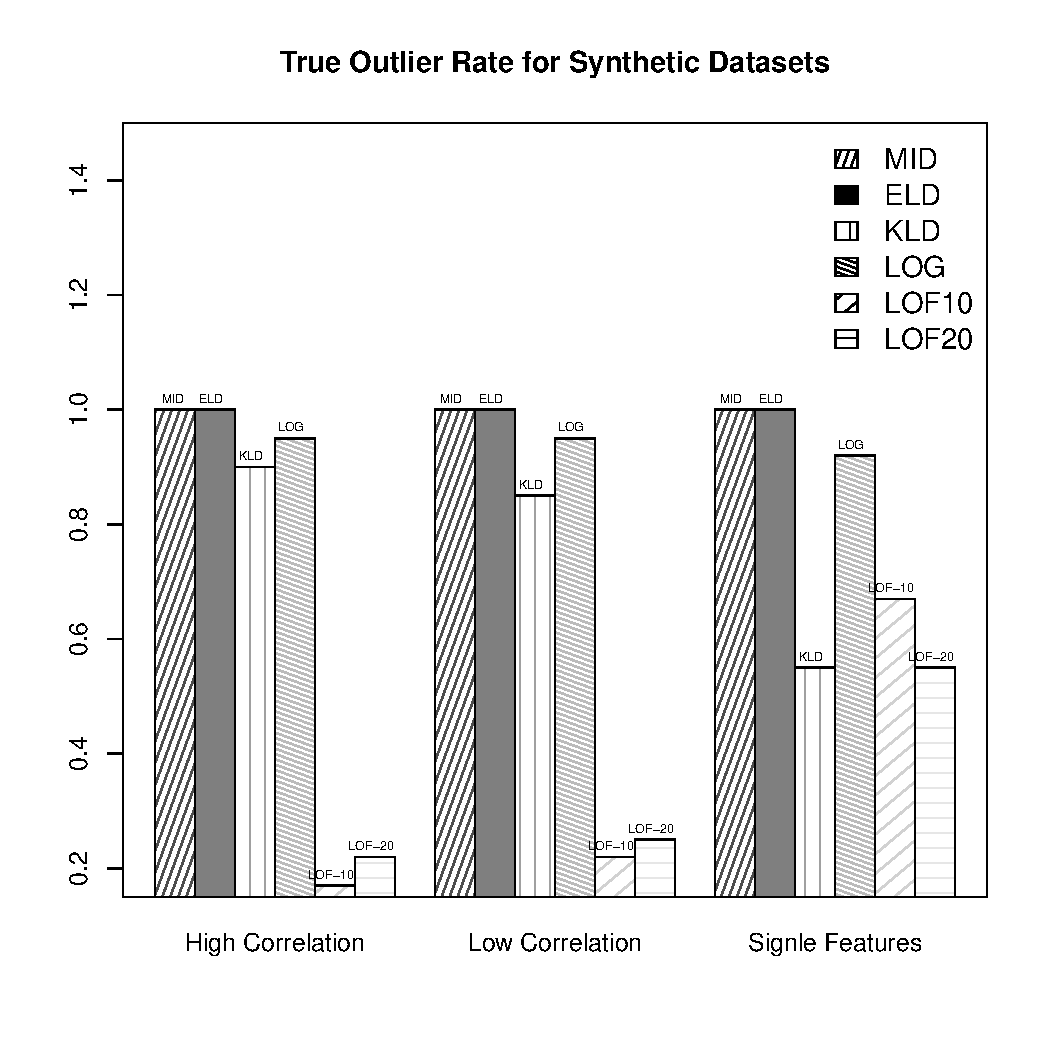
\includegraphics[height=70mm, width=70mm] {figures/TPR-Synthetic.pdf}
							%}
							%\subfigure{
							%  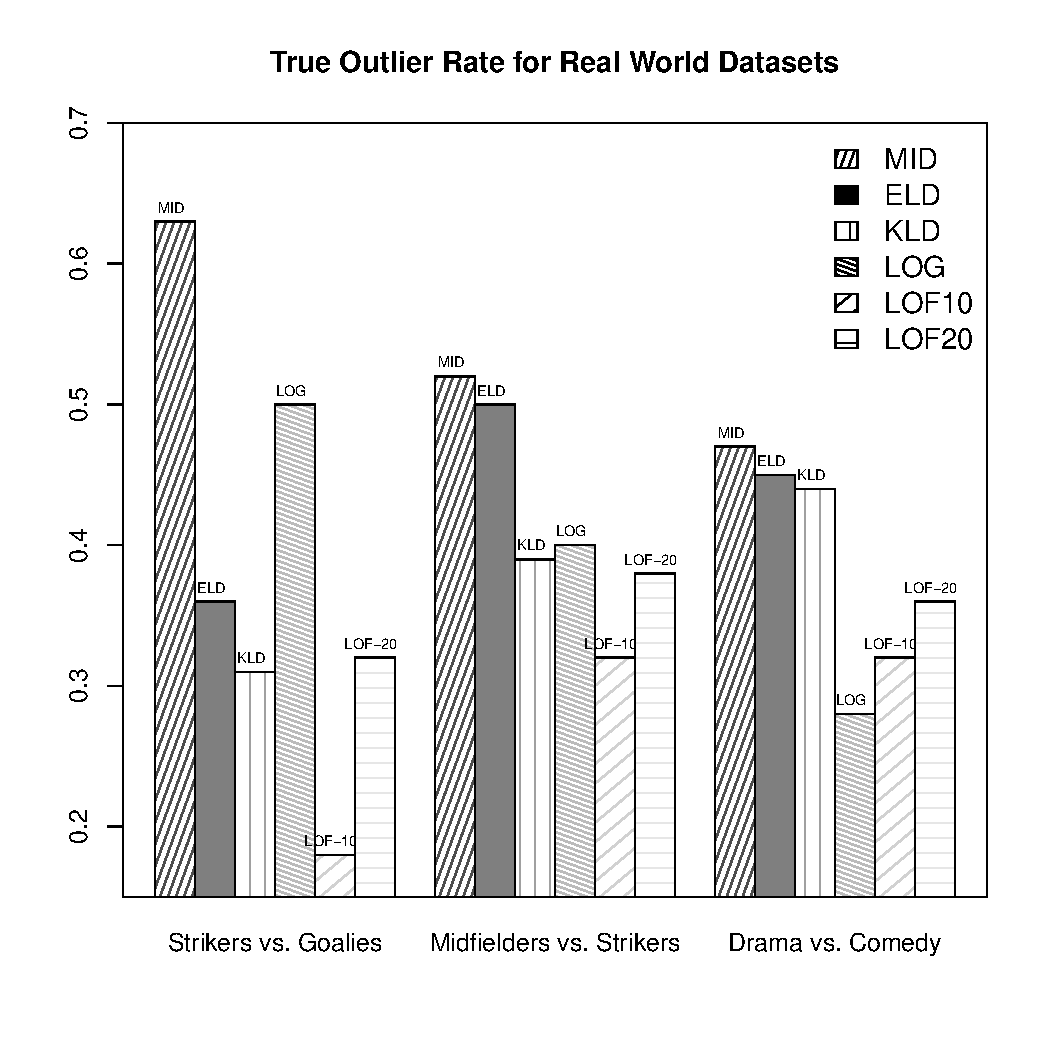
\includegraphics[height=70mm, width=70mm] {figures/TPR-All.pdf}
							
							% }
							% }
							
							%\caption{Comparison of Object Outlier Metrics}
							%\label{fig:synthetic}
							%\end{figure*}
							
							\subsubsection{Case Studies} For a case study, we examine three top outliers as ranked by $\mid$, shown in Table~\ref{table:CaseStudy}. 
							The aim of the case study is to provide a qualitative sense of the outliers indicated by the scores. Also, we illustrate how the BN representation leads to an interpretable ranking. 
							Specifically, we employ a {\em feature-wise decomposition} of the score combined with a {\em drill down} analysis: 
							
							\begin{enumerate}
								\item Find the node $\feature_{i}$ that has the highest $\mid_{i}$ divergence score for the outlier object. 
								\item Find the parent-child combination that contributes the most to the $\mid_{i}$ score for that node.
								\item Decompose the $\mid$ score for the parent-child combination into feature and mutual information component. 
							\end{enumerate}
							
							We present strong associations---indicated by the $\mid$'s mutual information component---in the intuitive format of association rules.
							
							%\begin{figure}
							%\centering
							%   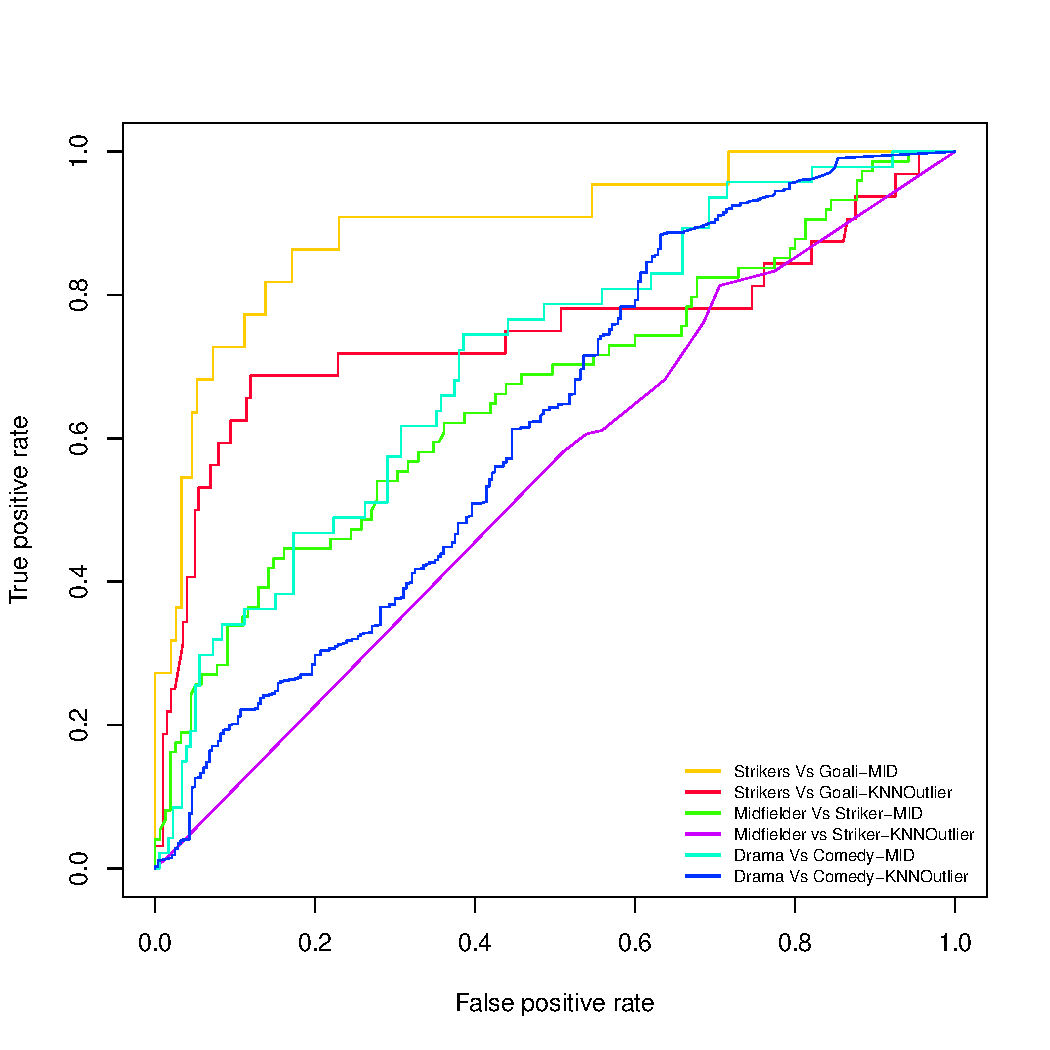
\includegraphics[width=0.5\textwidth] {figures/ROCKNN.pdf}
							% \caption{Detection Accuracy of $\mid$ vs. $\knn$
							% \label{fig:ROC}}
							%\end{figure}
							%\vspace{-5mm}
							\paragraph{Strikers vs. Goalies} 
							%The Mutual Information Score $\mid$ separates goalies from Strikers better compared to the other methods.  
							%
							In real-world data, a rare object may be a {\em within-class outlier}, i.e., highly anomalous even within its class. In an unsupervised setting without class labels, we do not expect an outlier score to distinguish such an in-class outlier from outliers outside the class. 
							%								This is the reason why in real-world data, we do not expect an outlier detection score to distinguish the normal class objects perfectly from objects outside the class. 
							An example is the striker Edin Dzeko. He is a highly anomalous striker who obtains 
							the top $\mid$ divergence score among both strikers and goalies. His $\mid$ score is highest for the Dribble Efficiency feature. The highest $\mid$ score for that feature occurs when Dribble Efficiency is low, and its parents have the following values: Shot Efficiency high, Tackle Efficiency medium. Looking at the single feature divergence, 
							%Decomposing this $\mid$ score into feature divergence and joint information divergence, 
							we see that Edin Dzeko is indeed an outlier in the Dribble Efficiency subspace: His dribble efficiency is low in 16\% of his matches, whereas a randomly selected striker has low dribble efficiency in 50\% of their matches. Thus, Edin Dzeko is an unusually good dribbler. Looking at the mutual information component of $\mid$, i.e., the parent-child correlations, for Edin Dzeko the confidence of the rule 
							$$\it{ShotEff} = \it{high}, \it{TackleEff} = \it{medium}\rightarrow \it{DribbleEff} = \it{low}$$ is 50\%, whereas in the general striker class it is $38\%$.
							%The $\eld$ divergence also ranks Edin Dzeko as unusual. But because it allows feature and joint information divergence to cancel, his rank is somewhat lower. The likelihood metric does not recognize him as unusual at all. 
							
							%								The next two outliers according to $\mid$ are goalies Paul Robinson and Michel Vorm. Their rank is based only on feature divergence, with zero mutual information distinction. The maximum feature divergence is obtained by the $\it{SavesMade}$ feature. This makes intuitive sense since strikers basically never make saves. 
							%In other words, feature divergence with respect to $\it{SavesMade}$ is a good way to distinguish goalies from strikers. 
							%
							%The $\eld$ divergence also ranks Paul Robinson and Michel Vorm as clear goalies.  The likelihood metric does not recognize Paul Robinson as unusual at all. 
							%\vspace{-5mm}
							\paragraph{Midfielders vs. Strikers} 
							%The  $\mid$ metric separates midfielders from strikers better compared than the other methods.  
							%The single feature divergence does not discriminate these two classes of objects. Intuitively, this is because strikers and midfielders are generally similar with respect to single features.  
							%The distance metrics have a better TOR rate than the averaging metrics. 
							
							%	The decomposition analysis for the top three $\mid$ outliers proceeds as follows. 
							For the single feature score, Robin van Persie is recognized as a clear striker because of the $\it{ShotsOnTarget}$ feature. It makes sense that strikers shoot on target more often than midfielders. Robin van Persie  achieves a high number of shots on targets in $34\%$ of his matches, compared to $3\%$ for a random midfielder. The mutual information component shows that he also exhibits  unusual correlations. For example, 
							the confidence of the rule
							$$\it{ShotEff} = \it{high}, \it{TimePlayed} = \it{high} \rightarrow \it{ShotsOnTarget} = \it{high}$$
							is 70\% for van Persie, whereas for strikers overall it is 52\%.
							%Both the $\eld$ metric and the $\lnlikelihood$ metric recognize Van Persie as a striker. 
							
							%								Wayne Rooney is recognized as a striker for similar reasons, but less clearly because he achieves a high number of shots on target less frequently. 
							The most anomalous midfielder is Scott Sinclair. His most unusual feature is $\it{DribbleEfficiency}$: For feature divergence, he achieves a high dribble efficiency $50\%$ of the time, compared to a random midfielder with $30\%$. 
							%The $\jid$ divergence shows that he also exhibits unusual correlations for DribbleEfficiency.
							%The $\eld$ divergence too ranks Scott Sinclair as an unusual midfielder, whereas the likelihood method places him in the middle of his class. 
							%\vspace{-5mm}
							\paragraph{Drama vs. Comedy} 
							%As with the other datasets, the  $\mid$ metric separates normal objects  from the contrast class better than the other methods.   
							The top outlier rank is assigned to the within-class outlier $\it{Brave Heart}$. Its most  unusual feature is  $\it{ActorQuality}$: In a random drama movie,  $42\%$ of actors have the highest quality level 4, whereas for $\it{Brave Heart}$ $93\%$ of actors achieve the highest quality level. 
							%The $\eld$ divergence also ranks $\it{Brave Heart}$ as an unusual drama, whereas the likelihood method places it in the middle of its class. 
							
							%based on user assigned ranking. 
							The  $\mid$ score identifies the comedies  $\it{Blues Brothers}$ and $\it{Austin Powers}$ as the top out-of-class outliers. 
							%	The main contributor to these rankings is the $\it{Cast\_Position}$ feature. 
							In a random drama movie,  $49\%$ of actors have casting position 3, whereas for $\it{Austin Powers}$ $78\%$ of actors have this casting position, and for $\it{Blues Brothers}$ $88\%$ of actors do. 
							%								These three movies also show unusual correlations for this feature with high divergence in the mutual information component (not shown in Table~\ref{table:CaseStudy}).
							\begin{table*}
								\centering
								\caption{Case study for the top outliers returned by the log-likelihood distance score \mid
									\label{table:CaseStudy}}
								\resizebox{1\textwidth}{!}{
									\begin{tabular}{|l|l|l|l|l|l|l|l|} \hline
										\multicolumn{8}{|c|}{Strikers (Normal) vs. Goalies (Outlier)}\\
										\hline
										PlayerName&Position&$\mid$ Rank&$\mid$ Max Node&$\mid$ Node Score&$\fd$ Max feature Value& Object Probability& Class Probability \\ \hline
										Edin Dzeko&Striker&1&DribbleEfficiency&83.84&DE=low&0.16&0.5 \\ \hline
										Paul Robinson&Goalie&2&SavesMade&49.4&SM=Medium&0.3&0.04\\ \hline
										Michel Vorm&Goalie&3&SavesMade&85.9&SM=Medium&0.37&0.04\\ \hline
										\multicolumn{8}{|c|}{Midfielders (Normal) vs. Strikers (Outlier)}\\
										\hline
										PlayerName&Position&$\mid$ Rank&$\mid$ Max Node&$\mid$ Node Score&$\fd$ Max feature Value& Object Probability& Class Probability \\ \hline
										Robin Van Persie& Striker&1&ShotsOnTarget&153.18&ST=high&0.34&0.03 \\ \hline
										Wayne Rooney& Striker&2&ShotsOnTarget&113.14&ST=high&0.26&0.03\\ \hline
										Scott Sinclair&Midfielder&6&DribbleEfficiency&71.9&DE=high&0.5&0.3\\ \hline
										\multicolumn{8}{|c|}{Drama (Normal) vs. Comedy (Outlier)}\\
										\hline
										MovieTitle&Genre&$\mid$ Rank&$\mid$ Max Node&$\mid$ Node Score& $\fd$ Max feature Value& Object Probability& Class Probability \\ \hline
										Brave Heart&Drama&1&ActorQuality&89995.4&a\_quality=4&0.93&0.42\\ \hline
										Austin Powers&Comedy&2&Cast\_Position&61021.28&Cast\_Num=3&0.78&0.49\\ \hline
										Blue Brothers&Comedy&3&Cast\_Position&24432.21&Cast\_num=3&0.88&0.49\\ \hline
									\end{tabular} 
								}
							\end{table*}
							\begin{figure*}[htbp]
								\centering
								\resizebox{0.85\textwidth}{!}{
									\includegraphics%[width=0.3\textwidth] 
									{figures/figure1kddCropped.pdf}
								}
								\caption{Illustrative Bayesian networks. The networks are not learned from data, but hand-constructed to be plausible for the soccer domain. (a) High Correlation: Normal individuals exhibit a strong association between their features, outliers no association. Both normals and outliers have a close to uniform distribution over single features.
									% The outlier distribution misses a correlation that is present in the normal population. The single feature distributions are uniform in both distributions. 
									(b) Low Correlation: Normal individuals exhibit no association between their features, outliers have a strong association. Both normals and outliers have a close to uniform distribution over single features.
									% The outlier object exhibits a correlation that is not present in the normal population. The single attribute distributions are uniform in both distributions.
									(c) Single Attributes: Both normal and outlier individuals exhibit a strong association between their features. In normals, 90\% of the time, feature 1 has value 0. For outliers, feature 1 has value 0 only 10\% of the time. 
									%Correlations are the same, but the single feature distributions are not.
									\label{fig:synthetic-bns}}
							\end{figure*}
							
\section{Correlation with Success}

Appearance of professional soccer statistics websites has made it possible to extend statistical studies to sports domain. One of the interesting problems in this domain is to predict success and present true estimates of individuals abilities. Market value varies for different players in various ages and nationalities. It is worth to study the factors that could have influence on market value of the players.\\
One easy way to estimate the value of the players may be to manually aggregate important features of them over time and then rank players based on those aggregated features. For example, we can compare the players based on the total number of goals they have scored or their shot efficiency. But this criterion may be unfair to most players as not all the players are in the position to shot or score a goal (e.g. goalies or defenders). One may argue that defenders (or goalies) have some other characteristics that are a lot stronger in their own group. However, knowing what features are more important for which category of individuals and how to treat the unimportant features is a hard task.  \\
Another disadvantage of manual aggregation method is that it is unable to identify the interactive attributes. By applying a generative model such as Bayesnet to soccer data we can see which interactive features are useful to process. For instance, number of matches that a player plays becomes important when the player shows high dribble efficiency and pass efficiency.  \\
In this section we use the likelihood ratio metric to rank the individuals. The data shows a surprisingly strong correlation between the ELD metric and individuals' success metrics.
\subsection{Preliminary Analysis}
We fist study a few independent variables that can possibly affect market value of the players and their ranking. We manually collected salary, nationality and age of 120 players of Premier League in order to investigate the effect of each of these factors on the success of the players.  
\paragraph{Fact \#1: Some teams tend to pay more:} Figure~\ref{fig:SalaryTeam} shows the distribution of salaries in different teams. Some teams have much larger
budgets and are able to pay higher wages compared to less wealthier teams. A player in ``Manchester United'' may not be necessarily performing substantially better than a player in the same position in ``Tottenhamham'', while there is a substantial difference between the average salary of players in Tottenham and Manchester United. Figure~\ref{fig:NormalizedSalary} shows that normalizing the salaries of the player can decrease this effect. Fortunately, after normalization, the difference between averages of salary paid by most of the teams is minor.% and we can expect this factor to have little effect on predicting the success.

\begin{figure}
	\centering     %%% not \center
	\subfigure[Wage bill of different teams]{\label{fig:SalaryTeam}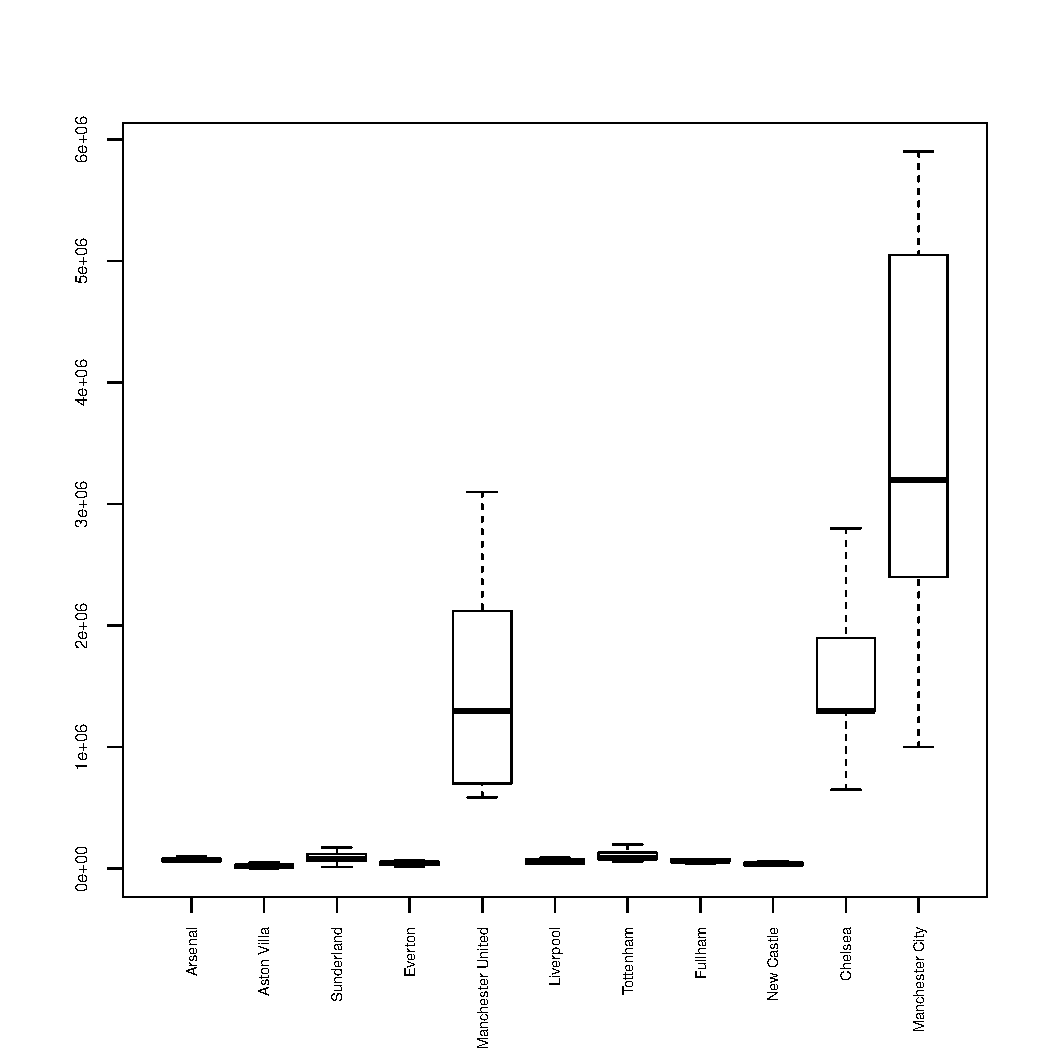
\includegraphics[width=55mm]{figures/TeamSal-2.pdf}}
	\subfigure[Wage bill different teams after normalization]{\label{fig:NormalizedSalary}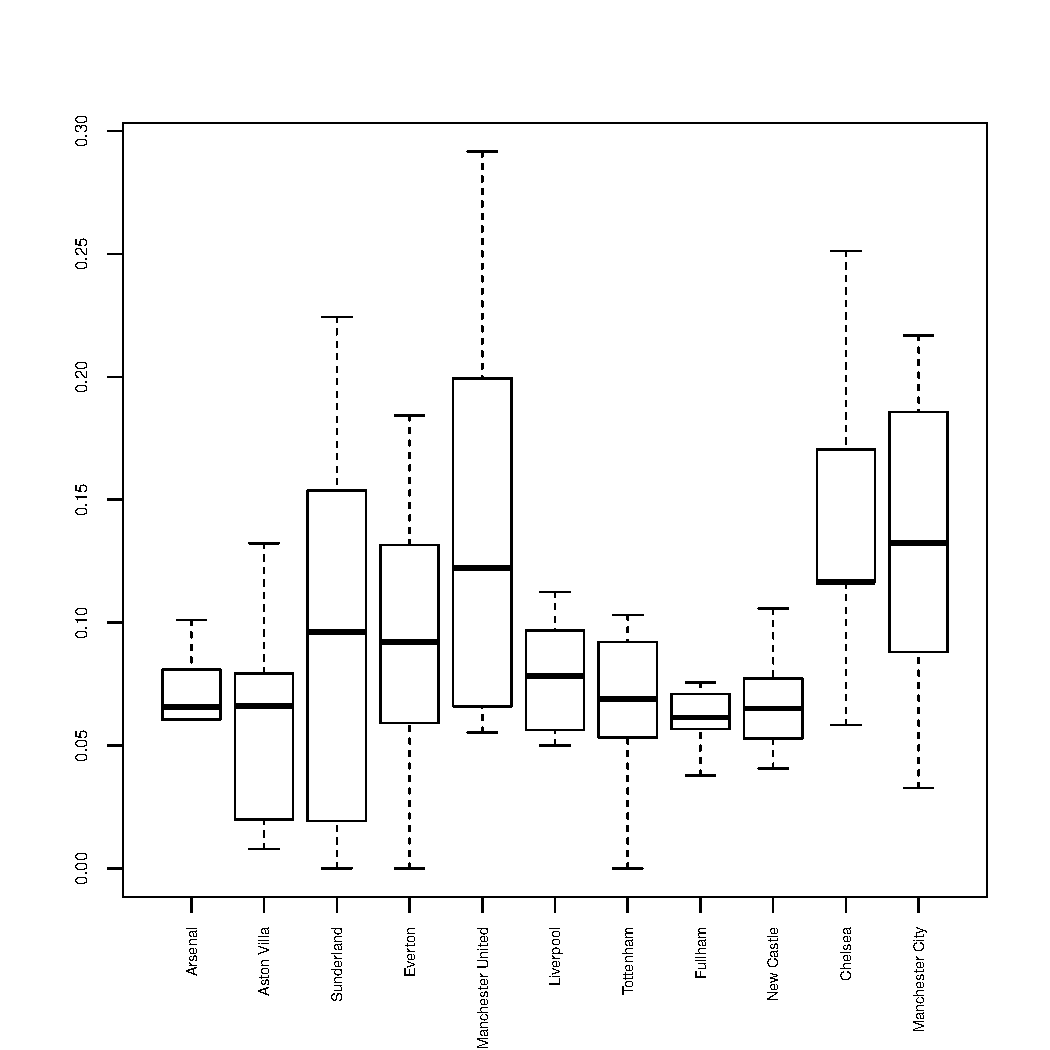
\includegraphics[width=55mm]{figures/TeamNormalSal-2.pdf}}
	\caption{Premier League wage bill: club-by-club}
\end{figure}

\paragraph{Fact \#2 Player's nationality has little effect on player's salary:} Previous research on Soccer shows that nationality of a player sometimes affects his salary regardless of his performance~\cite{Wooten2013}. \\
``The phrase `Brazilian soccer player' is like the phrases `French chef' or `Tibetan monk.'  The nationality
expresses an authority, an innate vocation for the job-whatever the natural ability.''~\cite{PAPASTERGIADIS2013}\\
We investigated the effect of this phenomenon in our domain and showed that it has very little effect on players market value. Figure~\ref{fig:PlayersNormalizedSalary}(a) shows the distribution of salaries of the players across different nationalities.


\begin{figure}
	\centering     %%% not \center
	\subfigure[	Salaries of players across different nationalities. ]{\label{fig:SalaryTeam}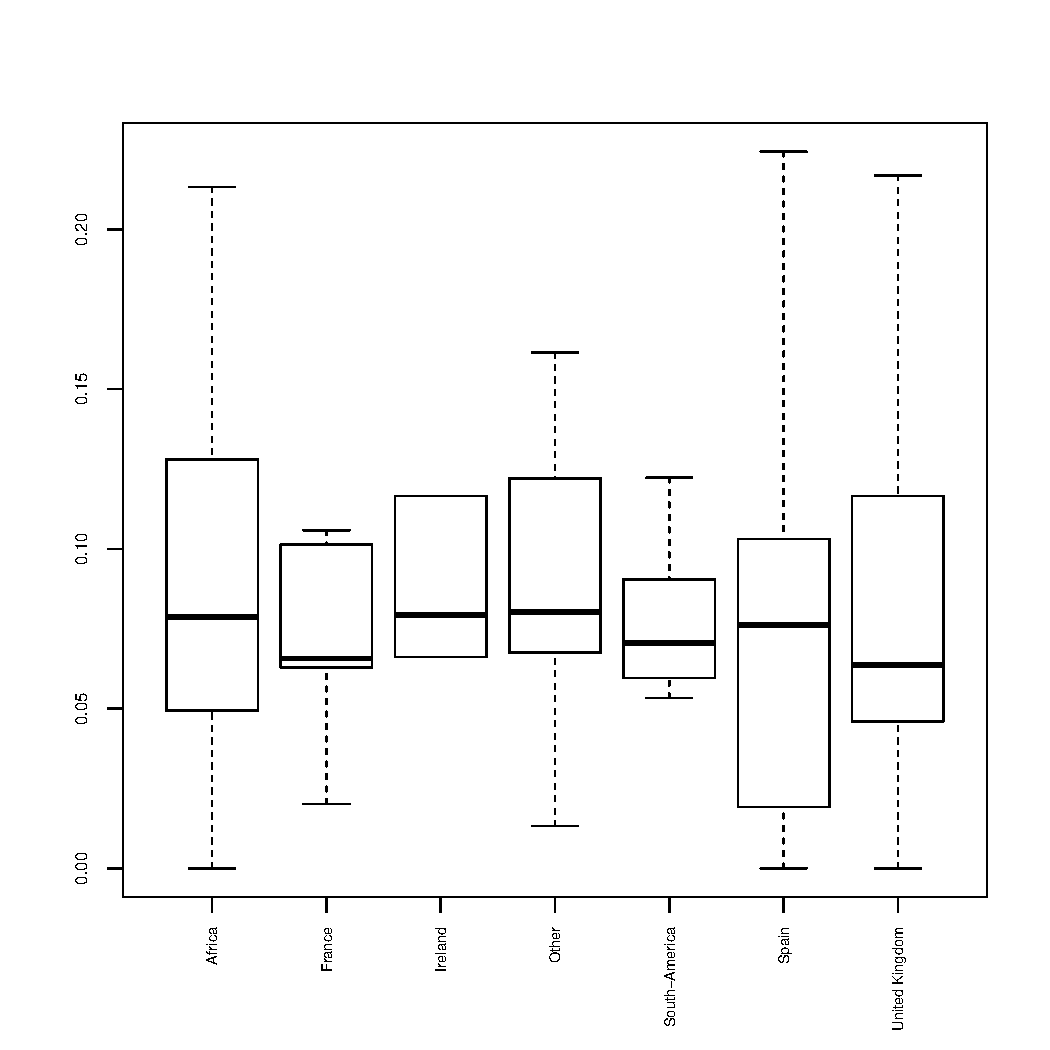
\includegraphics[width=55mm]{figures/nationalityNormalSal.pdf}}
	\subfigure[	Salaries of players in different ages. ]{\label{fig:b}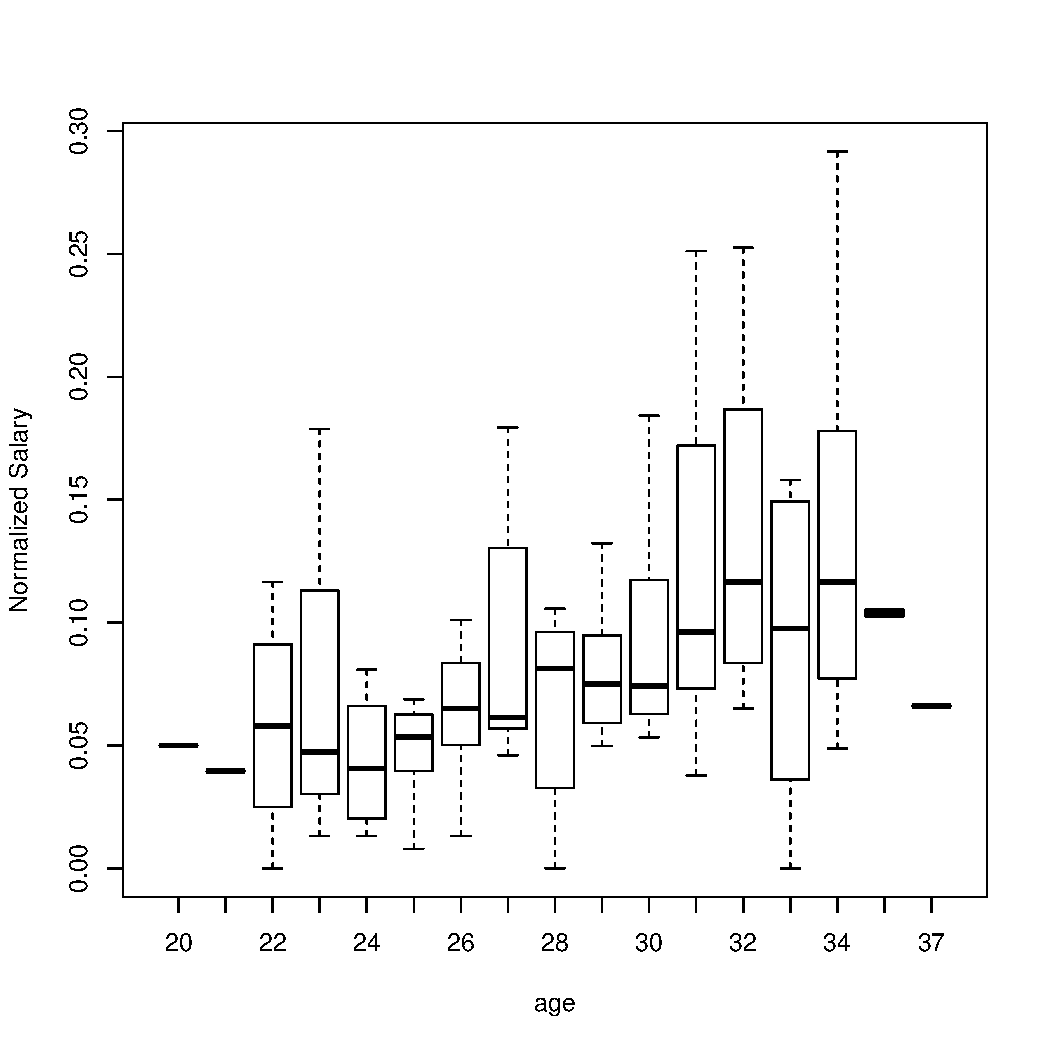
\includegraphics[width=55mm]{figures/PlayersNormalizedSalary.pdf}}
	\caption{Premier League wage bill: club-by-club}\label{fig:PlayersNormalizedSalary}
\end{figure}

%\begin{figure}[t]
%	\centering
%	\includegraphics[width=0.6\textwidth] 
%	{figures/nationalityNormalSal.pdf}
%	\caption{
%		Salaries of players across different nationalities. 
%		\label{fig:nationalitySalary}
%	}
%\end{figure}

\paragraph{Fact \#3 Player's salary increases as age increases:}
Older players from age 30 to 33 tend to earn higher wages compared to other age groups because it takes time to accumulate fame and experience. A famous player and a young player may play equally good but the famous player may have a higher salary due to his reputation. \\
For each player, salary distribution has a different peak but it is between 30-33 for most players~\cite{schwartz}. Figure~\ref{fig:PlayersNormalizedSalary}(b) shows the salary of the players in different ages.


\subsection{Related Work }
%Performance assessment is an important tool for operational analysts in many areas. For example, performance of traders or engineers is assessed by fund managers\cite{Grinblatt1989,Swamidass1987}.\\
\subsubsection{Analyzing sports data}
Analyzing sports data can make significant difference in scoring players, signing contracts and preventing injuries. Pei{~\em et al.}\cite{Pei2006} propose a reference based method that use relative degree of density with respect to a fixed set of reference points to calculate the neighborhood density of a data point. They aim to find outstanding players based on two test settings: 1) games player, goals scored and shooting percentages. 2) points scored, plus minus statistics and penalty minus. \\
Schwartz~\cite{schwartz} {~\em et al.} focused on the valuation of draft order in the SuperDraft. The valuation of draft order was first introduced in National Football League and proved to be very useful to the coach in trading players. They first estimate career trajectories of players and then assess the value of the draft position by introducing some performance measure. They used time played and salary of the player as ground truth in order to validate their method.


\subsubsection{Ranking system in Sports domain}
Ranking individuals is a useful for many applications in Information Retrieval, Natural Language Processing and Data mining.
In sports performance is usually interpreted as a rating system or ranking system. Ranking players is specially important in this domain because teams with lower budgets usually are looking for ways to detect undervalued players to be able to compete with wealthier teams for lower costs.
Lewis {\em et. al}~\cite{Lewis2003} used a quantitative analyst to value baseball players. \\
In the individual sports (e.g. tennis) ranking is straightforward and can be driven from the results of the past tournaments and it has been done by the Association of Tennis Professionals (ATP) for years. However, this simple framework for ranking has been questioned and claimed to perform poorly in predicting the results of future gams~\cite{McHale2011}. Other sports association such as soccer and cricket also have official rankings of teams and players which is the basis of many important decisions. For example, the FIFA world ranking plays an important part in awarding work permits to players outside the European Union in the Premier League~\cite{McHale2012}.
The problem of ranking teams and players is not trivial and the need of a better analytical system should not be understated.Although the world ranking performs poorly in predicting the match outcome,but it has been used to determine qualifications for tournaments\cite{McHale2007}.

In team sports rating individuals is a more complex task due to team structure. Players have different positions.Keri {\em et. al} have been developed a rating system for each speciality in Baseball~\cite{Keri2006}.

The analysis becomes more complicated when the goal is to compare players with different specialities. \cite{Goldman2010} investigates the metrics that attempt such an analysis in baseball and value players regardless of their position.
% Lewis 2005 has explored methodologies for such rating system for Cricket. 
McHale~\cite{McHale2012} {~\em et. al} developed an index to rate players regardless of their playing speciality based on player contribution to wining performances. 

%\subsection{Experiments}
\subsubsection{Datasets}
Similar to the other chapters, data tables are prepared from Opta data~\cite{opta-original} and IMDb~\cite{IMDBoriginal}. Table~\ref{table:Features} lists the populations and features. Table~\ref{table:Stats} shows summary statistics for the datasets. 
\begin{table}
	\centering
	\resizebox{0.8\textwidth}{!}{
		\begin{tabular}{|l|l|l|l|} \hline
			\multicolumn{2}{|c|}{Premier League Statistics}& \multicolumn{2}{|c|}{IMDB Statistics}\\
			\hline
			Number Teams&20&Number Movies&3060 \\ \hline
			Number Players&484&Number Directors&220 \\ \hline
			Number Matches&380&Number Actors&98690  \\ \hline
			avg player per match&26.01& avg actor per movie&36.42  \\ \hline
		\end{tabular} 
	}
	\caption{Summary Statistics for the IMDB and Soccer data sets}
	\label{table:Stats}
\end{table}


\begin{table}[htbp]
	\centering
	\resizebox{0.8\textwidth}{!}{
		\begin{tabular}{|c|p{5cm}|}
			\hline
			Individuals & Features\\ \hline
			\begin{tabular}{c}Soccer-Player\\per Match \end{tabular} & $\it{TimePlayed}$,$\it{Goals}$,$\it{SavesMade}$,
			$\it{ShotEff}$,$\it{PassEff}$,$\it{WinningGoal}$,
			$\it{FirstGoal}$,$\it{PositionID}$, $\it{TackleEff}$,$\it{DribbleEff}$,
			$\it{ShotsOnTarget}$ \\ \hline
			\begin{tabular}{c}Soccer-Team\\per Match \end{tabular} & $\it{Result}$,$\it{TeamFormation}$,
			$\sum\it{Goals}$,$\mu\it{ShotEff}$,$\mu\it{PassEff}$,
			$\mu\it{TackleEff}$,$\mu\it{DribbleEff}$. \\ \hline
			IMDB-Actor & $\it{Quality}$, $\it{Gender}$ \\ \hline
			IMDB-Director & $\it{Quality}$,$\it{avgRevenue}$\\ \hline
			IMDB-Movie&$\it{year}$,$\it{isEnglish}$,$\it{Genre}$,$\it{Country}$, $\it{RunningTime}$, $\it{Rating}$ by User\\ \hline
			IMDB-User& %$\it{Rating}$,
			$\it{Gender}$, $\it{Occupation}$.\\ \hline
		\end{tabular}}
		\caption{Attribute Features.% $\mu$ = average, $\\sum$ = sum. For relationships please see text.
			\label{table:Features}}
		
	\end{table}
\subsection{Likelihood Ratio and Success Metrics}
The aim of this section is to compare the ELD metric with other meaningful success metrics for comparing individuals. Our reference metrics are success rankings of individuals, shown in table~\ref{table:metrics}. Strong correlations between the ELD metric and meaningful success metrics provide evidence that the ELD metric is meaningful as well. We measure correlation strength by the standard correlation coefficient $\rho$. The coefficient ranges from -1 to 1, where 0 means no correlation and 1 or -1 indicates maximum strength~\cite{Fisher1921}.\\

Correlations are remarkable in at least two respects. 1) the strength of the correlation between the ELD metric and the success ranking are high: coefficients range from 0.3 to 0.82. (Oliver: correlation between ELD and movie rank is not as high as sum of ratings, should we just drop that or keep it? see table~\ref{table:movie}). 2) The trend holds across two different domains, different types of individuals and different success metrics. 
\begin{table}[htbp]
	
	\centering
	\resizebox{0.8\textwidth}{!}{
		\begin{tabular}{|l|l|l|l|l|l|}
			\hline
			Dataset&Success Metric&Min&Max&Standard Dev.&Mean\\ \hline
			IMDb & Sum of Rating & 1 & 14795 & 1600.22 & 1057.58\\ \hline
			Soccer-Player &TimePlayed& 5.0 & 3420 & 1015.69 & 1484.0\\ \hline
			Soccer-Player&Normalized Salary&0.007&0.28&0.620&0.100\\\hline
			Soccer-Player&Sum of Shot Efficiency&0&82&9.87&6.53\\\hline
			Soccer-Team &Standing& 1.0 & 20 & 5.91 & 10.5\\ \hline
			
		\end{tabular}}
		\caption{Success metrics. \label{table:metrics}}
		
	\end{table}
	\begin{figure}
		\centering
		\begin{minipage}{0.45\linewidth}
			\centering
			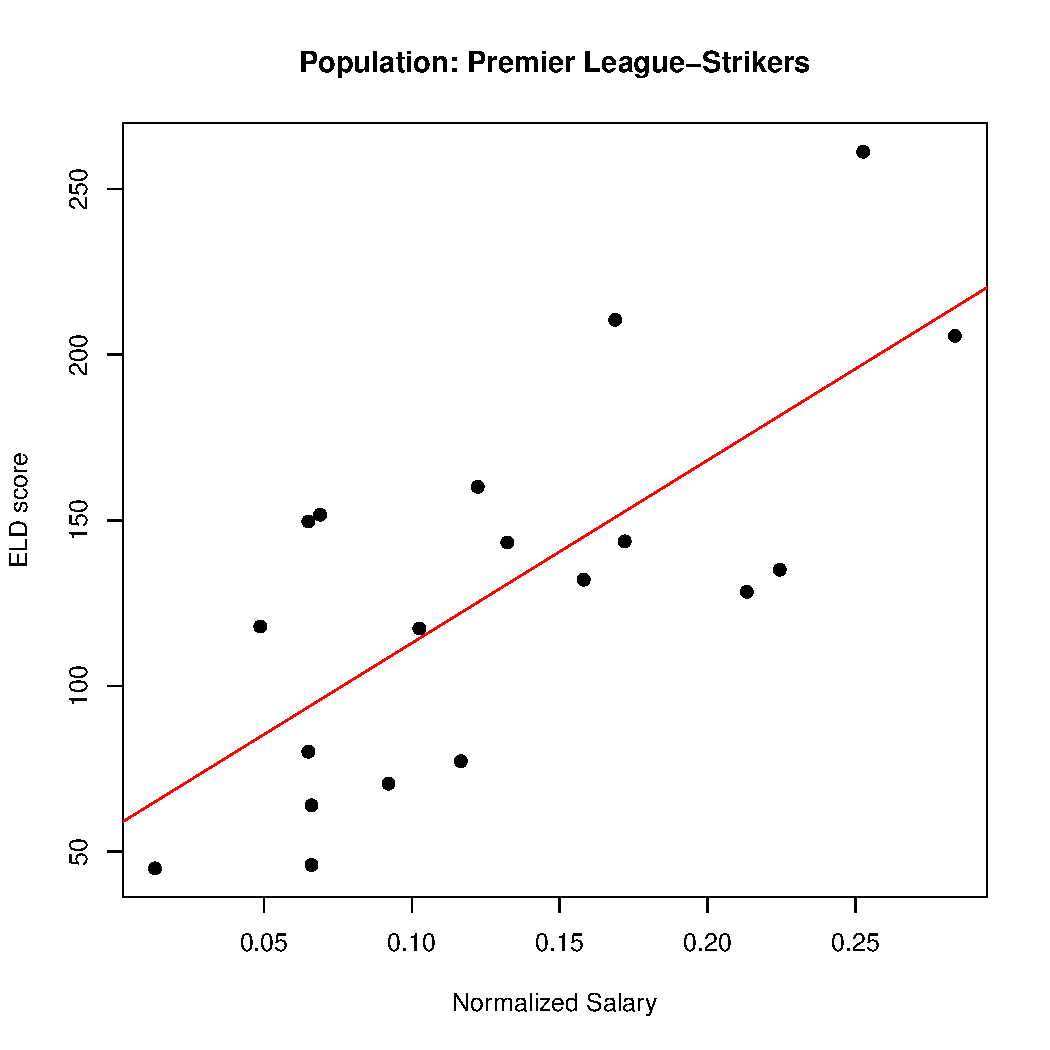
\includegraphics[width=2.5in]{Correlation-SimplePlots/1d-sumStrikerSalary.pdf}
			\caption{Strikers: Salary vs ELD}
			\label{fig:StrikerSalary}
		\end{minipage}
		\hspace{0.05\linewidth}
		\begin{minipage}{0.45\linewidth}
			\centering
			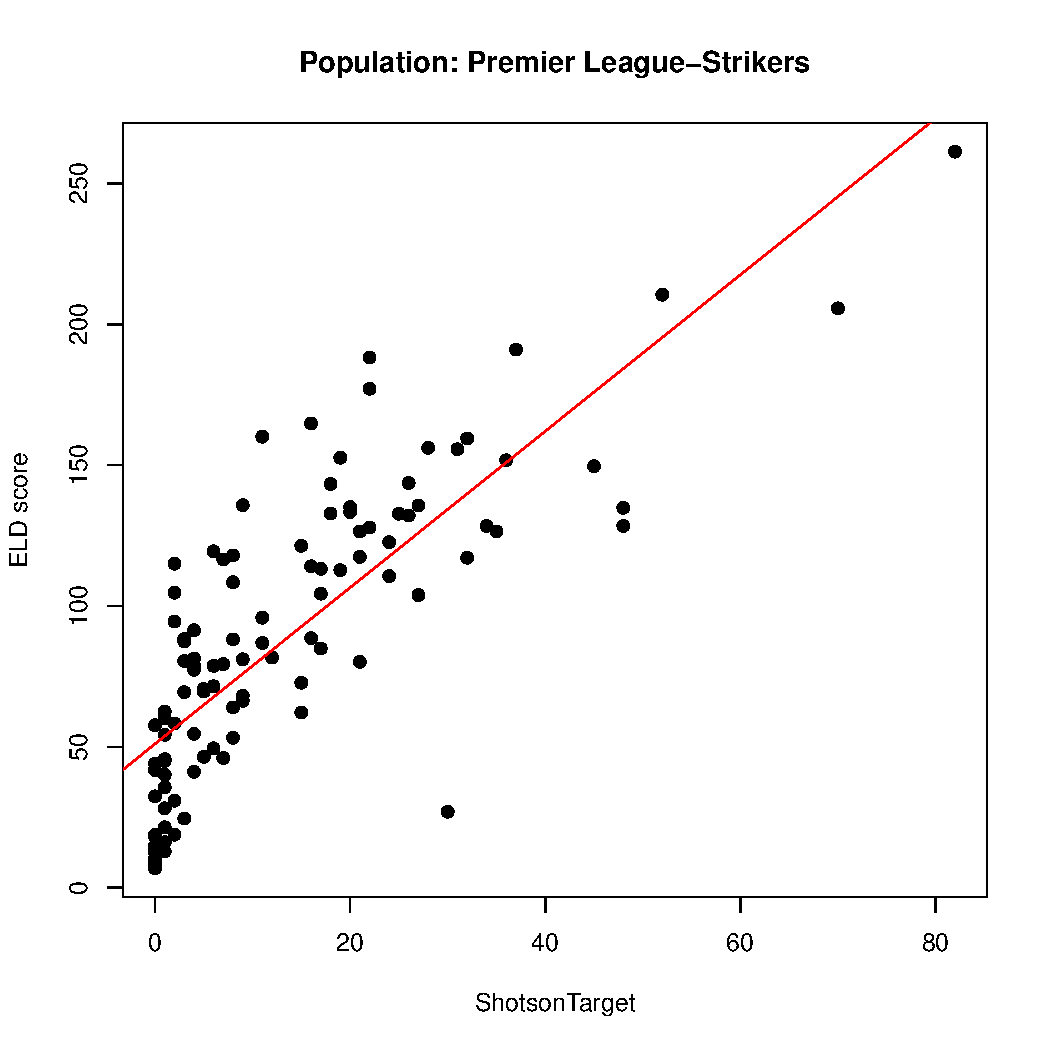
\includegraphics[width=2.5in]{Correlation-SimplePlots/1d-ShotsonTarget-sumStrikerStatistics.pdf}
			\caption{Strikers: Shots On Target vs ELD}
			\label{fig:StrikerShot}
		\end{minipage}
		\hspace{0.05\linewidth}
		\begin{minipage}{0.45\linewidth}
			\centering
			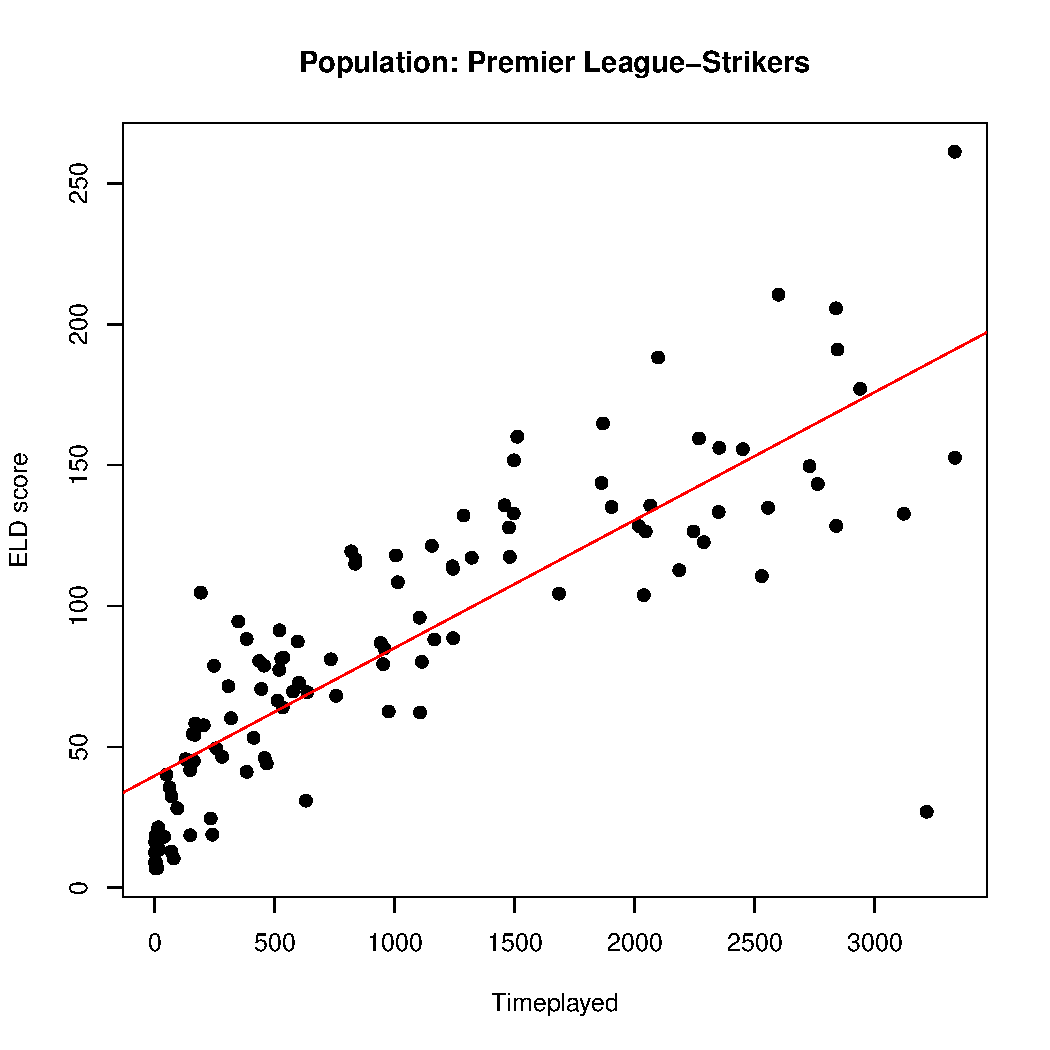
\includegraphics[width=2.5in]{Correlation-SimplePlots/1d-sumStrikerStatistics.pdf}
			\caption{Strikers: Time played vs ELD}
			\label{fig:StrikerTime}
		\end{minipage}
	\end{figure}
	
	\begin{figure}
		\centering
		\begin{minipage}{0.465\linewidth}
			\centering
			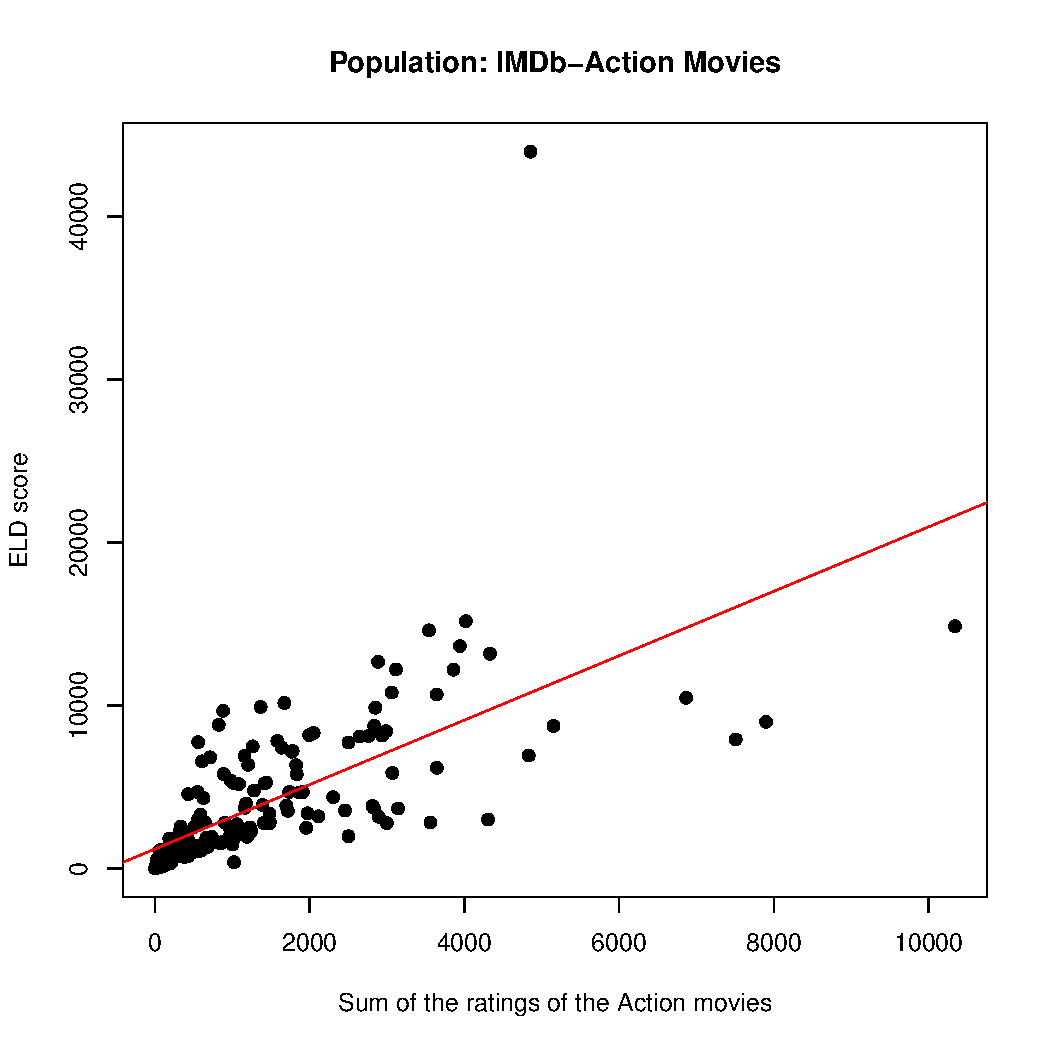
\includegraphics[width=2.5in]{Correlation-SimplePlots/Action-Correlation.pdf}
			\caption{Action movies: sum of ratings by users vs ELD}
			\label{fig:ActionRate}
		\end{minipage}
		\hspace{0.05\linewidth}
		\begin{minipage}{0.465\linewidth}
			\centering
			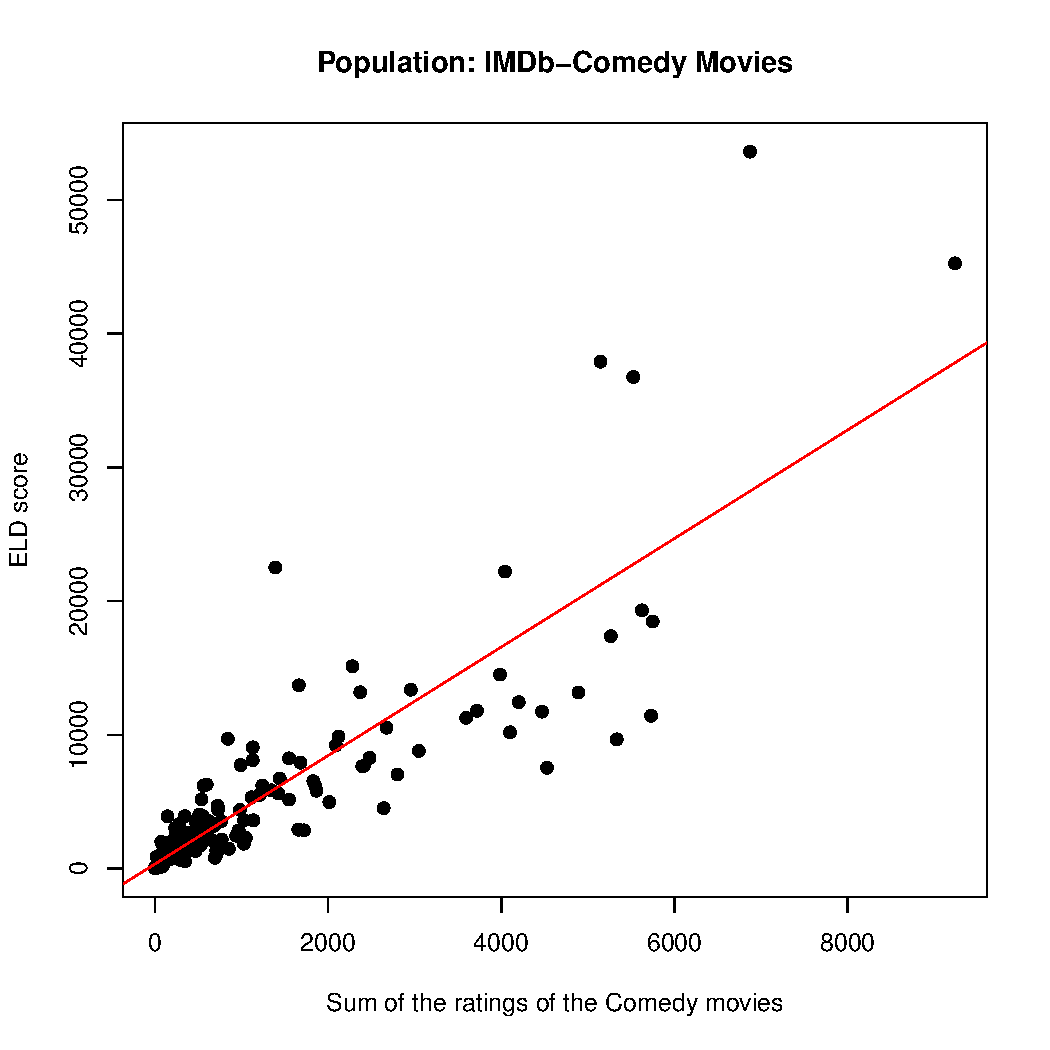
\includegraphics[width=2.5in]{Correlation-SimplePlots/Comedy-Correlation.pdf}
			\caption{Comedy movies: sum of ratings by users vs ELD}
			\label{fig:ComedyRate}
		\end{minipage}
		\hspace{0.05\linewidth}
		\begin{minipage}{0.465\linewidth}
			\centering
			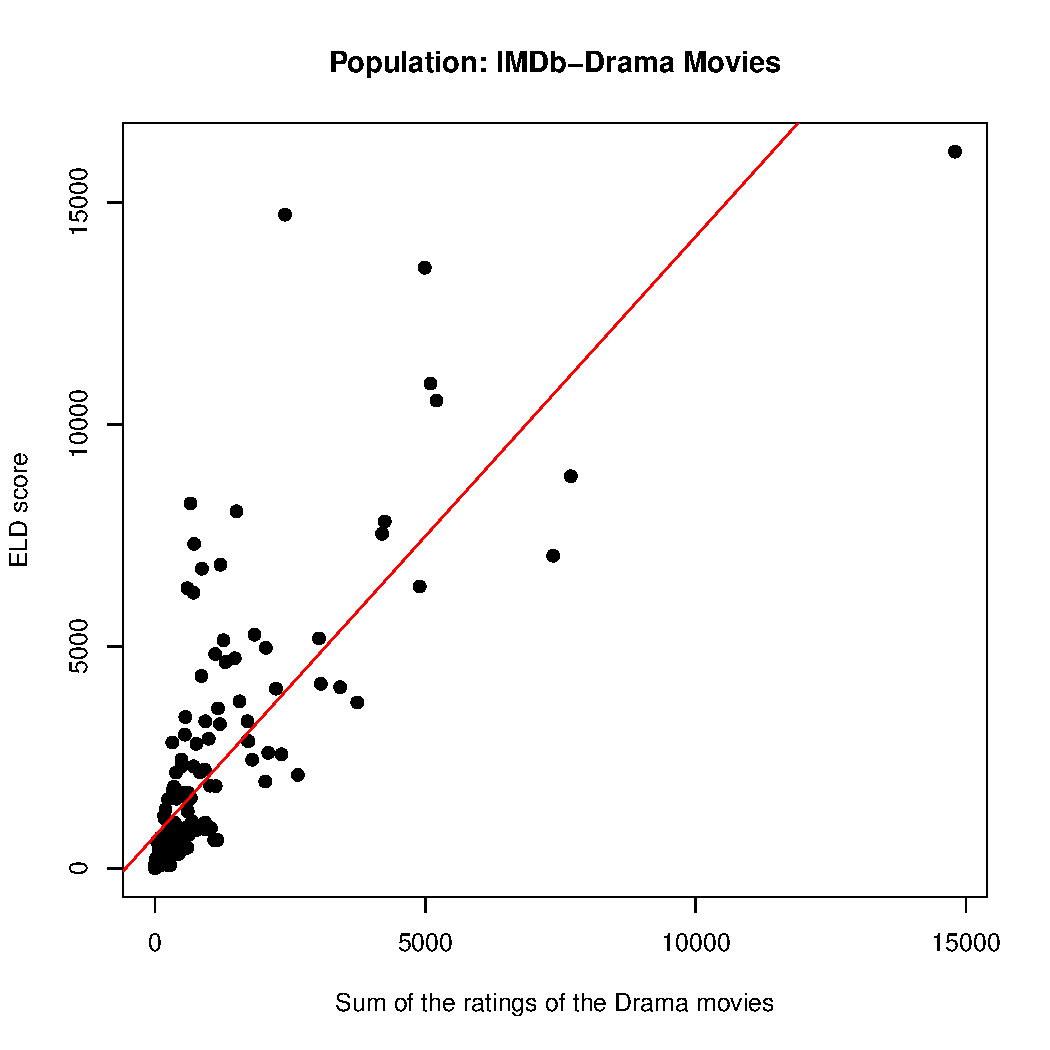
\includegraphics[width=2.5in]{Correlation-SimplePlots/Drama-Correlation.pdf}
			\caption{Drama movies: sum of ratings by users vs ELD}
			\label{fig:DramaRate}
		\end{minipage}
	\end{figure}
	
	
	
	
	\begin{figure}
		\centering
		\begin{minipage}{0.45\linewidth}
			\centering
			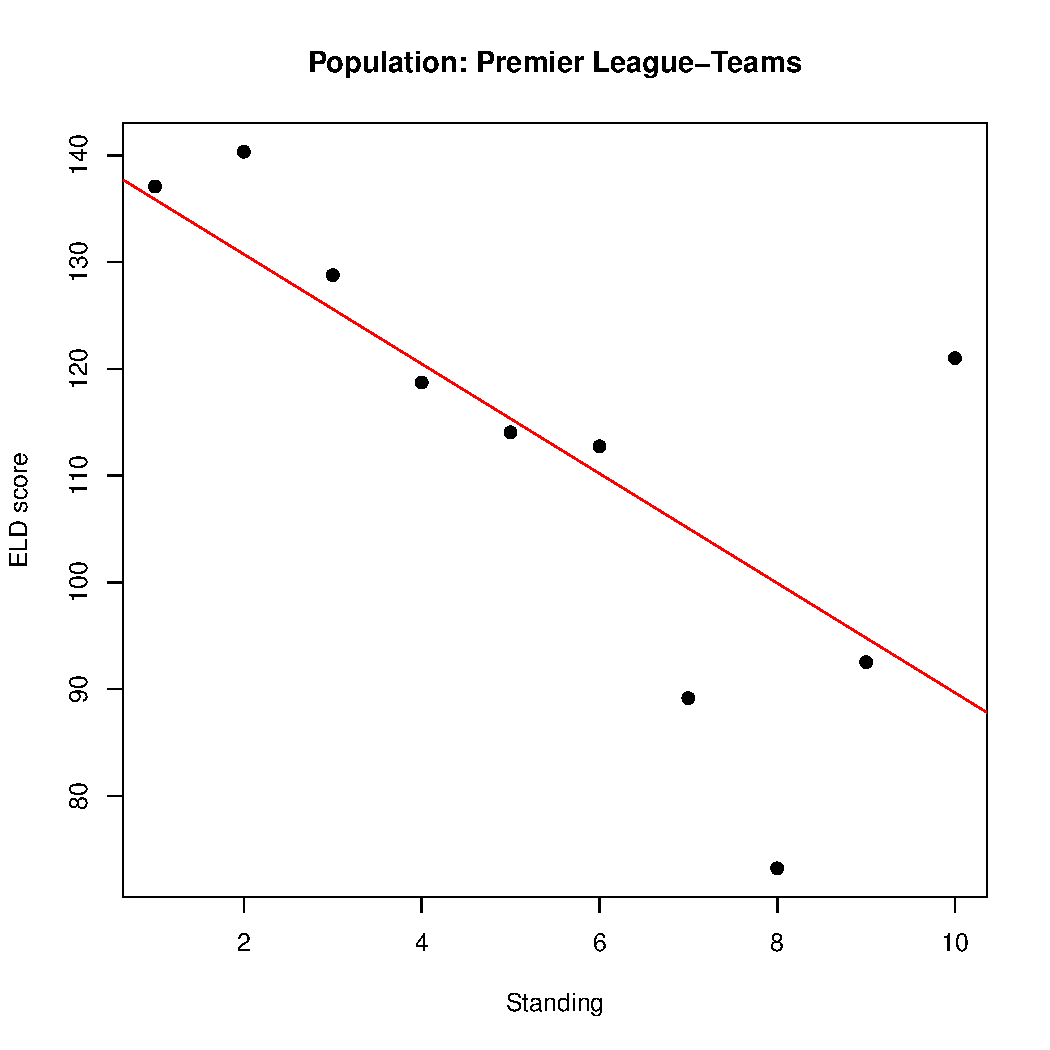
\includegraphics[width=2.5in]{Correlation-SimplePlots/TeamStanding.pdf}
			\caption{Teams: Correlation between team's Standing and ELD for the top teams in Premier League standing}
			\label{fig:teamStanding}
		\end{minipage}
		\hspace{0.05\linewidth}
		\begin{minipage}{0.45\linewidth}
			\centering
			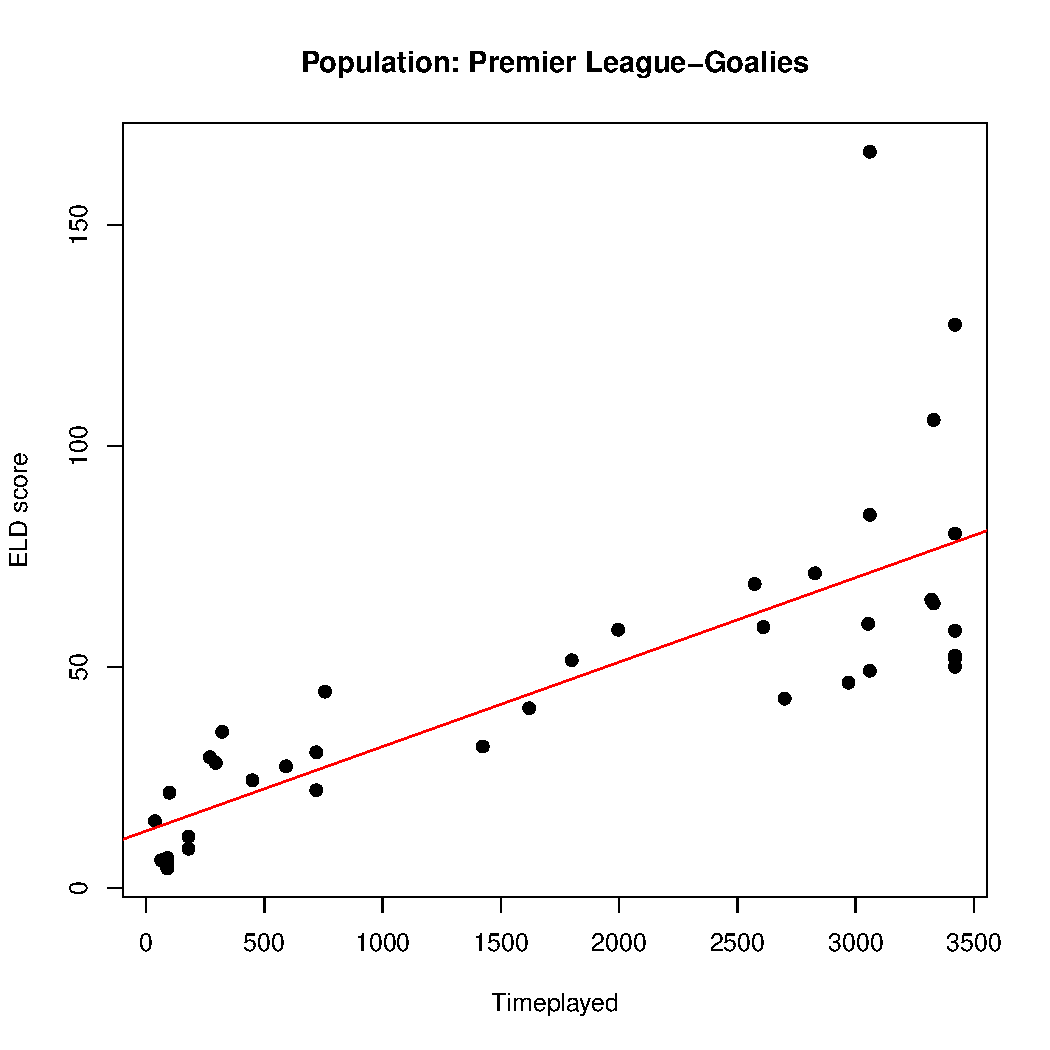
\includegraphics[width=2.5in]{Correlation-SimplePlots/sumGoalieStatistics.pdf}
			\caption{Goalies: sum of time played vs ELD}
			\label{fig:GoalieTime}
		\end{minipage}
		\hspace{0.05\linewidth}
		\begin{minipage}{0.45\linewidth}
			\centering
			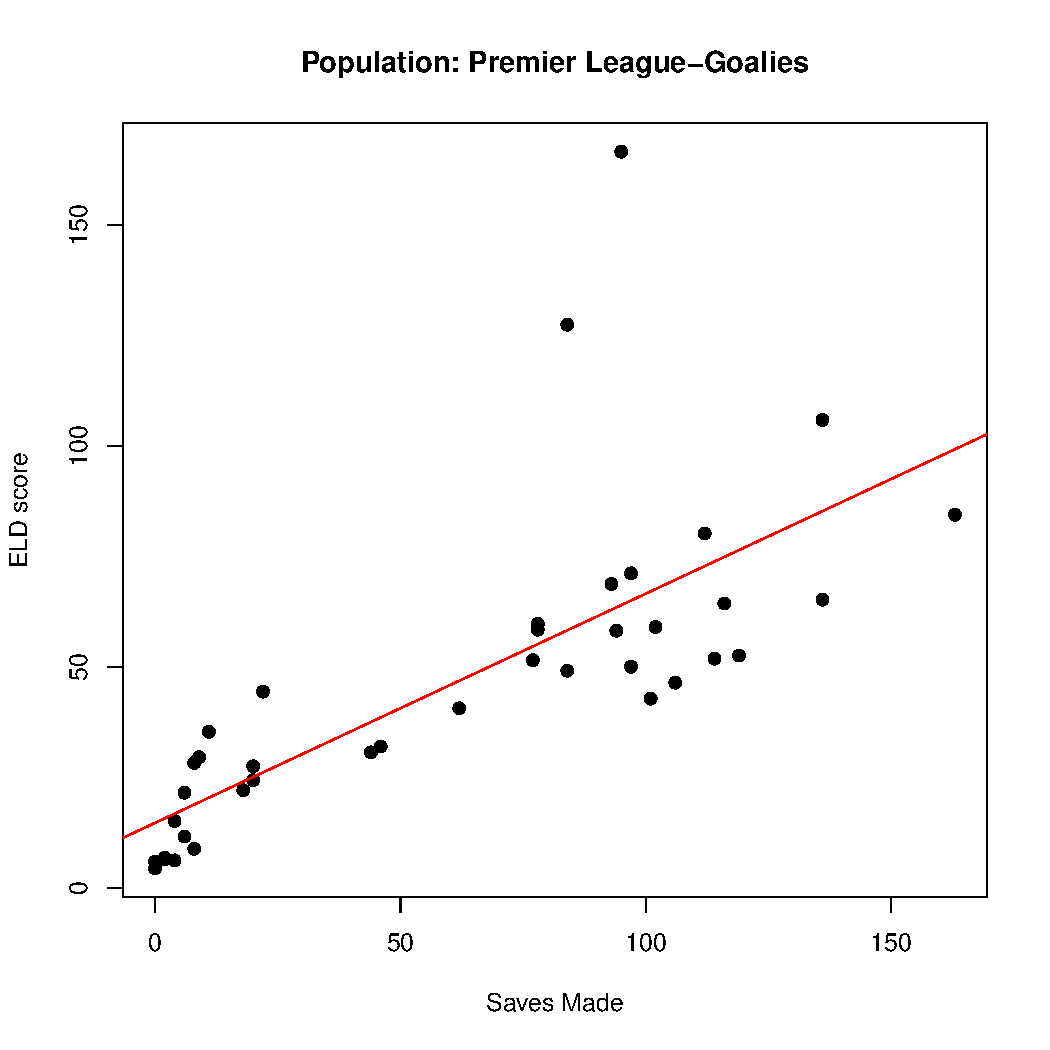
\includegraphics[width=2.5in]{Correlation-SimplePlots/sumGoalieStatisticsSavesMade.pdf}
			\caption{Goalies: sum of saves made by users vs ELD}
			\label{fig:GoalieSaves}
		\end{minipage}
	\end{figure}
	
	The quality of generalization of population is the key to the performance of ELD metric in ranking individuals. For example, in Premier League we expect most players to be in the range of good players. So the more different a player is from the population we can interpret it as a sign of detecting exceptionally good players. If we have a more diverse population in terms of performance, apart from a serious decline in quality of generation, being different from generic model can be interpreted as both exceptionally better or worst than normal population.\\
	Another point to consider is that, in BN generalization, similar to statistical generalization, population size and the structure of the  individuals is important. For example, in the Premier League, when the goal is to predict the success of  teams, there is no strong correlation between the ELD metric and standing of the teams as we expected it to be similar to the other domain/individuals ($\rho(Standing, ELD)=-0.21$). This could be due to the diverse and yet very small population (20 teams in total). But when we decrease diversity by considering only top 10 teams in our evaluation, correlation becomes a lot more stronger ($\rho(Standing, ELD)=-0.71$).
	\paragraph{Team Standing}
	The most successful team has Standing=1 and the least successful team has Standing=20. If we distinguish top teams in the standing, a strong negative correlation emerges between ELD and standing: teams with higher ELD achieve a better(lower) standing. Figure~\ref{fig:teamStanding} shows the scatter plot of this correlation and its best fit regression line.
	\paragraph{Players Time Played} is the total time that a player played over all matches in the season. This metric was shown to correlate strongly with other success metrics, such as salary, on MLS soccer data~\cite{schwartz}. Tables ~\ref{table:goalie} and \ref{table:strikers} and Figures \ref{fig:GoalieTime} and \ref{fig:StrikerTime} show the correlation between the ELD metric and time played. For the entire population there is a strong positive correlation meaning that atypical players with higher ELD tend to play more minutes.
	\paragraph{Salary} is probably the most obvious and at the same time can be the most misleading measure to compare players. We manually collected salaries of some players that we could find on-line. Table \ref{table:strikers}  and Figures~\ref{fig:NormalizedSalary} show the correlation between ELD and this success metric.
	\paragraph{Shots on Target} is any shot attempt that would or does enter the goal if left unblocked. We record total number these shots over all matches of the players. This metric was shown to correlate strongly with ELD (see Table \ref{table:strikers}, Figure~\ref{fig:StrikerShot}).
	\paragraph{Saves Made} is total number of saves that goalies had made over all the matches. This metric has been used as another success metric for Goalies' population and shows a strong correlation as well(see Table ~\ref{table:goalie}, Figure\ref{fig:GoalieSaves}).  
	\paragraph{Movie Rating} is the sum of user rating of the movies. For the movies in different Genre this metric shows a high correlation with the ELD metric (see Table~\ref{table:movie}, Figure~\ref{fig:ActionRate},Figure~\ref{fig:ComedyRate}, Figure~\ref{fig:DramaRate}).
	\begin{table}[htbp]
		
		\centering
		\resizebox{0.7\textwidth}{!}{
			\begin{tabular}{|c|c|c|c|}
				\hline
				Metric&Sum of SavesMade&TimePlayed&Salary\\\hline
				ELD&0.71&0.73&0.6\\\hline
			\end{tabular}}
			%
			\caption{Correlation between ELD metric and success metric of Goalies .\label{table:goalie}}
		\end{table}
			\begin{table}[htbp]
				
				\centering
				\resizebox{0.7\textwidth}{!}{
					\begin{tabular}{|c|c|c|c|}
						\hline
								Metric&Sum of Pass Efficiency&TimePlayed&Salary\\\hline
								ELD&0.78&0.68&0.38\\\hline
					\end{tabular}}
					%
					\caption{Correlation between ELD metric and success metric of Midfielders .\label{table:Midfielders}}
				\end{table}
		\begin{table}[htbp]
			
			\centering
			\resizebox{0.7\textwidth}{!}{
				\begin{tabular}{|c|c|c|c|}
					\hline
					Metric&Shots On Target&TimePlayed& Salary\\\hline
					ELD&0.72&0.82&0.79\\\hline
				\end{tabular}}
				%
				\caption{Correlation between ELD metric and success metric of Strikers .\label{table:strikers}}
			\end{table}
			
			
			\begin{table}[htbp]
				
				\centering
				\resizebox{0.5\textwidth}{!}{
					\begin{tabular}{|c|c|c|}
						\hline
						Genre&Sum of Rating&Movie Rank\\\hline
						Action&0.68&0.30\\\hline
						Drama&0.78&0.31\\\hline
						Comedy&0.85&0.42\\\hline
					\end{tabular}}
					%
					\caption{Correlation between ELD metric and success metric of Movies .\label{table:movie}}
				\end{table}
				
				%	\begin{figure}[t]
				%		\centering
				%		\includegraphics[width=0.8\textwidth] 
				%		{correlations/Drama-Correlation.pdf}
				%		\caption{
				%			Salaries of players across different nationalities. 
				%			\label{fig:nationalitySalary}
				%		}
				%	\end{figure}			
				%\begin{figure}



%					\be
%Comparing Equations~\eqref{eq:lr+} and~\eqref{eq:mid-bn} we see that the $\mid$ score is obtained from the $\lr^{+}$ score by using absolute values of differences (in our notation, $\mid = |\lr^{+}|$. A standard result in information theory states that a joint distribution can, without loss of information, be decomposed into a univariate distribution and the multi-variate mutual information. This implies that the decomposed KLD score $\lr^{+}$ is identical to $\lr$. 
%the distinction between $\lr$ and $\mid$ is as follows: $\lr$ computes the expected log-{\em differences}, whereas $\mid$ computes the expected log-{\em distances}. Many standard divergence measures for distributions \cite{Chan2004} compute expected differences; we argue that for outlier detection, {\em one should compute expected distances instead.} The fundamental reason is that averaging differences is appropriate when considering costs, payoffs or utilities, but not appropriate when assessing the distinctness of an object. For example, $\lr$ can be interpreted as the average difference in message length when data points are encoded following the class distribution rather than the object distribution \cite{Tuffery2011}.
%\cite{Witten2005}. 
%If we treat message length as a cost, then $\lr$ computes the average cost of using the class distribution rather than the object distribution. 
%Some message lengths are shorter in the class distribution, some in the object distribution, and these differences cancel out. Since our goal is to assess the distinctness of an object, {\em we do not want differences to cancel out.}

%The next proposition shows that the outlier scores have the standard properties of a divergence measure between probability distributions: they are nonnegative, and 0 if and only if the class and object distributions are the same. Also, the triangle inequality entails that the scores can be ordered by dominance: one is guaranteed to be at least as great as another. Dominance means that a divergence potentially provides more discrimination among objects as it maps the set of objects onto a larger range of scores. Our $\mid$ score dominates all others.  We provide empirical evidence that dominance does correspond to greater discrimination.
%
%\begin{mydef} Assume maximum likelihood estimation for the object-level parameters $\parameters_{\object}$. Then for any class and object distribution, we have $\mid \geq |\lr| \geq \lr = \lr^{+} \geq 0$. The outlier scores are 0 if and only if the the object and class distribution are the same; otherwise, all inequalities are strict.
%\end{mydef}
%
%{\em Proof Outline.} The inequalities all follow from the triangle inequality $|a|+|b|\geq |a+b|$. The equality $\lr = \lr^{+}$ follows by applying the decomposition~\ref{eq:decompose}. The maximum likelihood parameters maximize the function $\loglikelihood(\D_{\object},\model_{\Class},\cdot)$ \cite{Schulte2012}, so the log-likelihood ratio $\lr$ is positive if and only if $\theta_{\Class} = \theta_{\parameters}$.
%\vspace{-5mm}
%\paragraph{Computational Complexity} Assume that for each joint assignment of values $\set{x}$, the object probability $P_{\object}(\set{x})$ and the class probabilities $P_{\class}(\set{x})$ can be computed in linear time (e.g., by a table lookup). Then the computational complexity of evaluating the $\mid$ score is bounded by the number of joint assignments $\prod_{i=1}^{n} \states_{i}$. This term grows exponentially with the number of attributes. In the next section we discuss how the computational cost of evaluating the score can be greatly reduced by employing a Bayesian network representation of the class and object distributions. 



%\section{Bayesian Network Representation}\label{sec:bn}
%
%
%
%
%
%Given a BN representation of the object and class distribution, the $\mid$ score is computed as follows: 
%
%$\begin{array}{l} 
%%\sum_{j=1}^{\states_{i} P_{\object}(\feature_{i} = \nodevalue_{ij}) \left|\ln \frac{P_{\object}(\feature_{i} = \nodevalue_{ij})}\right| + \\
%%\sum_{i=1}^{n} \sum_{j=1}^{\states_{i}}P_{\object}(\feature_{i}=\nodevalue_{ij}) \ln \frac{P_{\object}(\feature_{i} = \nodevalue_{ij})}{P_{\Class}(\feature_{i} = \nodevalue_{ij})} +\\
%\mid =\sum_{j=1}^{\states_{i}} \parameter_{\object}( \nodevalue_{ij}) \left|\ln \frac{P_{\object}( \nodevalue_{ij})}{\parameter_{\Class}( \nodevalue_{ij})}\right|+\\
%\sum_{i=1}^{n}\sum_{j=1}^{\states_{i}} \sum_{\parents_{i}} 
%P_{\object}( \nodevalue_{ij},\parents_{i})
%\left|\ln \frac{\parameter_{\object}( \nodevalue_{ij}|\parents_{i})}{\parameter_{\object}(\nodevalue_{ij})} - \ln \frac{\parameter_{\Class}( \nodevalue_{ij}|\parents_{i})}{\parameter_{\Class}(\nodevalue_{ij})}\right|.
%\end{array}$
%
%We emphasize that Equation~\eqref{eq:mid-bn} is not a new outlier score compared to Equation~\eqref{eq:mid}. It is the same score using the Bayesian network factorization~\eqref{eq:bn} of the $\mid$ divergence~\eqref{eq:mid}. We derive Equation~\ref{eq:mid-bn} by starting with the BN expression of the KL divergence \cite{Neapolitan2004}, then apply the mutual information decomposition as in Equation~\ref{eq:kld-transform}, finally average log-distances rather than log-differences.  
%%\vspace{-5mm}
%\paragraph{Motivation} It is well-known that compared to a flat table representation of a joint distribution, the factored BN representation~\eqref{eq:bn} can be and typically is exponentially smaller \cite{Pearl1988}. Our experiments show this compression effect empirically  (Table~\ref{table:Number of Parameters}). With the BN representation, the $\mid$ score can be computed in time and space cost linear in the number of the conditional probability parameters in the object and class BNs. This typically provides an exponential reduction in computation cost compared to the tabular representation~\eqref{eq:mid}. 
%
%
%%Since the score decomposes into a sum, we can easily find the local factors that have the highest impact on it. This means that the $\mid$ score provides a kind of {\em subspace analysis.} Subspace analysis aims to find ascertain which subset of attributes contributes the most to a given outlier score. A standard approach searches for attribute subsets that are irrelevant in that eliminating them makes little difference to the outlier ranking. As our case study in the following illustrates, the BN metric supports finding the attributes with the most impact on the outlier score without the need for searching the space of attribute subsets. 
%
%In addition to compactness, another advantage of the BN representation is {\em interpretability}. Interpretability is very important for outlier detection. The BN form of the $\mid$ score is easily interpreted because it {\em decomposes} into a sum of {\em local} factors. Each multi-attribute local factor is based on the relevance of a small set of parent conditions for predicting the value of the child node. This relevance term is basically the same as the widely used lift measure \cite{Tuffery2011}, therefore an intuitively meaningful quantity. The $\mid$ score compares how relevant a given parent condition is in the object profile with how relevant it is in the general class. 
%the conditional probability parameters correspond to {\em local} features that describe the conditional distribution of a single variable given a fairly small set of parent values. 
%The Bayes net advantages of compactness and interpretability carry over to the $\mid$ score, as 




%Since the score decomposes into a sum, we can easily find the local factors that have the highest impact on it. This means that the $\mid$ score provides a kind of {\em subspace analysis.} Subspace analysis aims to find ascertain which subset of attributes contributes the most to a given outlier score. A standard approach searches for attribute subsets that are irrelevant in that eliminating them makes little difference to the outlier ranking. As our case study in the following illustrates, the BN metric supports finding the attributes with the most impact on the outlier score without the need for searching the space of attribute subsets. 
%
%In our experiments we use Bayesian networks to represent the joint distributions for an object and its class. Our outlier metrics can also be defined in terms of generic joint distributions, without assuming that the distributions are represented by a Bayesian network. Our experiments use Bayesian network representations as well, so the formulas we present show the computations used in our evaluation.

%
% Using Bayesian networks to represent joint distribution has two key advantages \cite{Pearl1988}. (1) Compactness: the number of conditional probabilities that need to be specified is typically much less than the total number of joint probabilities. 
%% For instance, if the BN contains $n$ binary nodes, there are $2^{n}$ joint probabilities. If each node has a relatively small number $k$ of parents (a typical maximum is $k=5$), the number of parameters is only $n \cdot 2^{k}$, basically linear compared to the full set of $2^{n}$ numbers for specifying the joint probabilities directly. 
% %
% (2) Interpretability: the conditional probability parameters correspond to {\em local} attributes that describe the conditional distribution of a single variable given a fairly small set of parent values. The Bayes net advantages of compactness and interpretability carry over to object-oriented outlier metrics, which we discuss next.
%



%\begin{acknowledgements}
%If you'd like to thank anyone, place your comments here
%and remove the percent signs.
%\end{acknowledgements}

% BibTeX users please use one of
%\bibliographystyle{spbasic}      % basic style, author-year citations
%\bibliographystyle{spmpsci}      % mathematics and physical sciences
%\bibliographystyle{spphys}       % APS-like style for physics
%\bibliography{}   % name your BibTeX data base

% Non-BibTeX users please use
%\begin{thebibliography}{}
%%
%% and use \bibitem to create references. Consult the Instructions
%% for authors for reference list style.
%%
%\bibitem{RefJ}
%% Format for Journal Reference
%Author, Article title, Journal, Volume, page numbers (year)
%% Format for books
%\bibitem{RefB}
%Author, Book title, page numbers. Publisher, place (year)
%% etc
%\end{thebibliography}
			\bibliographystyle{abbrv}
			\bibliography{Bibliography-File,master}
\end{document}
% end of file template.tex

